%% 
%% Copyright 2019-2024 Elsevier Ltd
%% 
%% This file is part of the 'CAS Bundle'.
%% -------------------
%% 
%% It may be distributed under the conditions of the LaTeX Project Public
%% License, either version 1.3c of this license or (at your option) any
%% later version.  The latest version of this license is in
%%    http://www.latex-project.org/lppl.txt
%% and version 1.3c or later is part of all distributions of LaTeX
%% version 1999/12/01 or later.
%% 
%% The list of all files belonging to the 'CAS Bundle' is
%% given in the file `manifest.txt'.
%% 
%% Template article for cas-sc documentclass for 
%% double column output.

\documentclass[a4paper,fleqn]{cas-sc}

\usepackage{algorithm}
\usepackage{algorithmic}
\usepackage{graphicx}
\usepackage{array}
\usepackage{url}
\usepackage{booktabs}
\usepackage{amssymb}
\usepackage{tikz}
\usetikzlibrary{positioning,fit,backgrounds,arrows.meta}


\usepackage{float}
\usepackage[section]{placeins}
\usepackage{flafter}

\setcounter{topnumber}{5}
\setcounter{bottomnumber}{5}
\setcounter{totalnumber}{10}

\renewcommand{\topfraction}{0.95}
\renewcommand{\bottomfraction}{0.90}
\renewcommand{\textfraction}{0.05}
\renewcommand{\floatpagefraction}{0.80}

% FROZEN v1 ARCHIVE.  This directory is a snapshot of the manuscript as it
% stood at the close of the first revision round (59 pages, tectonic exit 0).
% Its figures are pinned to the local v1/figures/ copies taken at that moment,
% NOT to ../../figures/, which the v2 rewrite is free to change.  Do not
% repoint this to the live figure directory: the whole purpose of v1 is that
% it still compiles to the same PDF after v2 has moved on.
% figs/ is searched second and holds the Elsevier sample graphics plus the
% superseded submitted-version copies of sensitivity_heatmap.png and
% morris_scatter.png.
\graphicspath{{figures/}{figs/}}

% If the frontmatter runs over more than one page
% use the longmktitle option.

%\documentclass[a4paper,fleqn,longmktitle]{cas-sc}

%\usepackage[numbers]{natbib}
%\usepackage[authoryear]{natbib}
\usepackage[authoryear,longnamesfirst]{natbib}

%%%Author macros
\def\tsc#1{\csdef{#1}{\textsc{\lowercase{#1}}\xspace}}
\tsc{WGM}
\tsc{QE}
%%%

% Uncomment and use as if needed
%\newtheorem{theorem}{Theorem}
%\newtheorem{lemma}[theorem]{Lemma}
%\newdefinition{rmk}{Remark}
%\newproof{pf}{Proof}
%\newproof{pot}{Proof of Theorem \ref{thm}}

\begin{document}
\let\WriteBookmarks\relax
\def\floatpagepagefraction{1}
\def\textpagefraction{.001}

% Short title
\shorttitle{A coupled Farquhar-Jarvis whole-plant simulation model}

% Short author
% >>> TODO(AUTHOR): replace with "F. Lastname et~al." <<<
\shortauthors{}

% Main title of the paper
\title [mode = title]{A coupled Farquhar-Jarvis whole-plant simulation
model: modular formulation, solver verification and global sensitivity
analysis}

% Title footnote mark
% (Re-enable together with \tnotetext[1] below if a funding or
%  acknowledgement note is required. An empty \tnotetext produces a
%  dangling footnote mark, so both are commented out.)
% \tnotemark[1]

% Title footnote 1.
% eg: \tnotetext[1]{Title footnote text}
% \tnotetext[1]{}

% First author
%
% Options: Use if required
% eg: \author[1,3]{Author Name}[type=editor,
%       style=chinese,
%       auid=000,
%       bioid=1,
%       prefix=Sir,
%       orcid=0000-0000-0000-0000,
%       facebook=<facebook id>,
%       twitter=<twitter id>,
%       linkedin=<linkedin id>,
%       gplus=<gplus id>]

% >>> TODO(AUTHOR): all author, affiliation, e-mail and ORCID fields below
%     are placeholders and MUST be filled in before submission. Elsevier
%     Editorial Manager will reject the PDF if the author line is empty.
%     An empty \author{} argument also suppresses the whole author block
%     in \MaketitleBox, which is one of the reasons the compiled PDF
%     showed no by-line. <<<
\author[1]{AUTHOR ONE}%[orcid=0000-0000-0000-0000]

% Corresponding author indication
\cormark[1]

% Footnote of the first author
% (Re-enable together with \fntext[1] below if an author footnote is needed.)
% \fnmark[1]

% Email id of the first author
% >>> TODO(AUTHOR): institutional e-mail of the corresponding author <<<
\ead{author.one@example.edu}

% URL of the first author
% \ead[url]{}

% Credit authorship
% >>> TODO(AUTHOR): CRediT roles per author; \printcredits at the end of
%     the document types them out, so leaving these empty prints nothing. <<<
\credit{Conceptualization, Methodology, Software, Investigation, Writing -- original draft}

% Address/affiliation
% >>> TODO(AUTHOR): fill affiliation 1 <<<
\affiliation[1]{organization={AFFILIATION ONE},
            addressline={},
            city={},
%          citysep={}, % Uncomment if no comma needed between city and postcode
            postcode={},
            state={},
            country={}}

% >>> TODO(AUTHOR): if the paper has a single author, delete this second
%     \author block, the \fnmark[2]/\ead{} lines and \affiliation[2]
%     entirely; do not leave them empty. <<<
\author[2]{AUTHOR TWO}%[]

% Footnote of the second author
% \fnmark[2]

% Email id of the second author
% >>> TODO(AUTHOR): institutional e-mail of the second author <<<
\ead{author.two@example.edu}

% URL of the second author
% \ead[url]{}

% Credit authorship
% >>> TODO(AUTHOR): CRediT roles for the second author <<<
\credit{Conceptualization, Supervision, Writing -- review \& editing}

% Address/affiliation
% >>> TODO(AUTHOR): fill affiliation 2 <<<
\affiliation[2]{organization={AFFILIATION TWO},
            addressline={},
            city={},
%          citysep={}, % Uncomment if no comma needed between city and postcode
            postcode={},
            state={},
            country={}}

% Corresponding author text
\cortext[1]{Corresponding author}

% Footnote text
% (Re-enable together with \fnmark[1]/\fnmark[2] above if needed.)
% \fntext[1]{}

% For a title note without a number/mark
%\nonumnote{}

% NOTE(compile) -- why the previous PDF showed no title and no abstract.
%
% Two independent causes, both now addressed:
%
% 1. Title and author. \title[mode=title]{} and \author[1]{} were literally
%    empty above, so \maketitle had nothing to typeset. \shorttitle and
%    \shortauthors were empty as well, which is why the running heads were
%    blank too. Filled in / marked TODO above.
%
% 2. Abstract. In the CAS classes the abstract is NOT typeset where it is
%    written. cas-common.sty renews the abstract environment as
%    \verbatimwrite{\jobname.abs} ... \endverbatimwrite (moreverb), i.e. the
%    body is written verbatim to an external file, and \MaketitleBox later
%    re-reads it with \file_if_exist:nT {\jobname.abs} { \file_input:n {...} }.
%    Because the test is \file_if_exist:nT, a missing or unreadable .abs file
%    is skipped silently: LaTeX reports no error and the abstract simply does
%    not appear. This happens when the .abs file cannot be written or cannot
%    be found again under \jobname -- typically when the build is run with a
%    separate output directory (latexmk -outdir / TeXstudio build subfolder)
%    that is not on the input search path, when auxiliary files are cleaned
%    between passes, or when moreverb.sty is not installed in the TeX tree.
%    Fix: build in the source directory (or add the aux directory to
%    TEXINPUTS), do not clean between passes, and confirm that
%    "kpsewhich moreverb.sty" resolves. If the abstract still does not appear,
%    check that <jobname>.abs exists and is non-empty after the first pass.
%
% Here goes the abstract
\begin{abstract}
Whole-plant growth simulation requires environmental forcing, leaf gas exchange, carbohydrate storage, nutrient uptake and biomass allocation to be advanced together over the diel cycle, yet many whole-plant and crop simulators prescribe the photosynthetic carbon input instead of computing it from the gas exchange on which the rest of the model depends. We reformulate a whole-plant, Tedone-based physiological framework as a modular coupled simulation model in which Farquhar-von Caemmerer-Berry photosynthesis and Jarvis stomatal conductance compute the carbon input, propagated into an eleven-state system of cytosolic and vacuolar sucrose, transient starch, nitrogen and phosphorus pools, and leaf and root biomass. The implicit gas-exchange constraint is solved in closed form: the coupled supply-demand system is a quadratic in the intercellular CO$_2$ concentration. The fixed-point iteration it replaces is retained as a switchable alternative and verified against it, revealing a period-two orbit below a leaf water potential of $-1.15$~MPa in which the sign of the assimilation rate depends on the iteration cap, and non-convergence in $15.2\%$ of sensitivity-design draws. The carbohydrate budget, integrated alongside the state equations, closes to a relative residual below $1.3\times10^{-14}$. For \textit{Arabidopsis thaliana} the model captures the diel starch cycle within a normalised-RMSE threshold of $0.25$ across 4-12~h photoperiods; the per-photoperiod relative growth rate (RGR) fit is saturated, and a held-out photoperiod test over 14 cross-validated fits gives a mean absolute percentage error of $28.5\%$ for photoperiod-independent coefficients, falling to $7.3\%$ once one coefficient is allowed to vary linearly with photoperiod --- reported here as the predictive figure of merit, and locating the model's photoperiod dependence in a single calibrated growth coefficient rather than in the coupled dynamics. An ablation study shows that computing rather than prescribing the carbon input removes a systematic RGR underestimation of up to $23\%$. A Sobol' analysis, its estimator first verified against a function with closed-form indices, attributes the majority of growth variance to parameter interactions --- the interaction remainder exceeds the first-order index in 44 of the 52 influential parameter-photoperiod cells --- and shows control shifting from nutrient uptake and respiration under short days to photosynthetic and light-supply capacity under long days. Alongside the simulation core we report verification tests that need no observational data and that found four defects invisible at the calibrated operating point, including an adaptive integrator step that stalls without diverging --- a failure mode invisible to any check formulated on the values the integrator produces.
\end{abstract}

% Use if graphical abstract is present
%\begin{graphicalabstract}
%\includegraphics{}
%\end{graphicalabstract}

% Research highlights
% (Elsevier limits highlights to 3-5 items of at most 85 characters each.)
\begin{highlights}
\item Whole-plant simulator couples Farquhar-Jarvis gas exchange to eleven state equations.
\item Analytic $C_i$ solution replaces a fixed point that cycles under water stress.
\item Sobol' estimator verified against a closed-form benchmark before use on the model.
\item Carbon budget closes to relative residuals below $1.3\times10^{-14}$ over all photoperiods.
\item Out-of-sample photoperiod tests replace an earlier, calibration-bound RGR agreement.
\end{highlights}


% Keywords
% Each keyword is seperated by \sep
\begin{keywords}
Coupled simulation model \sep
Modular model architecture \sep
Numerical verification \sep
Global sensitivity analysis \sep
Photosynthesis-growth coupling \sep
Plant growth simulation
\end{keywords}

\maketitle

% Main text
\section{Introduction}
\label{sec:introduction}

Simulating the growth of a whole plant requires several physical and biological subsystems to be updated together over time: environmental forcing must drive leaf gas exchange, the resulting carbon must be partitioned between transient reserves and mobile sugars, sugars must support nutrient uptake and maintenance, and the remaining assimilate must be allocated to new biomass. Each of these subsystems has an established modelling literature, but their behaviour is only biologically meaningful when they are coupled: the carbon available for growth at any instant is the outcome of the environment, the photosynthetic machinery and the internal carbohydrate and nutrient state acting together \cite{Farquhar1980,ThornleyJohnson1990}. For simulation, the main difficulty is therefore not any single process equation but the construction of a stable numerical workflow in which these processes exchange fluxes consistently over the day-night cycle. Photoperiod makes this problem clear: changing the day length alters the ratio of the light phase, during which carbon is assimilated and stored, to the dark phase, during which growth depends entirely on the mobilisation of stored starch \cite{Scialdone2013,Graf2010}, so a correctly coupled model should reproduce the shape of this shifting day-night balance across photoperiods from a single mechanism. We state this as the aspiration it is rather than as an achieved property: the model reported here requires two coefficients to be recalibrated per photoperiod, and Section~\ref{sec:results} quantifies how much of the photoperiod response that recalibration carries.

The individual physiological components needed for such a model are well established. The Farquhar-von Caemmerer-Berry biochemical model \cite{Farquhar1980} and Jarvis-type stomatal conductance \cite{Jarvis1976} describe leaf-level gas exchange, whole-plant and crop simulators such as APSIM, DSSAT and WOFOST integrate growth over field scales \cite{Holzworth2014,Jones2003,deWit2019}, and day-night starch turnover in \textit{Arabidopsis thaliana} has been characterised in detail \cite{Scialdone2013,Stitt2012}. In many of these whole-plant and crop simulators, however, the carbon input is still prescribed or strongly simplified, supplied as a light-use-efficiency term, a look-up table or an externally imposed assimilation rate, rather than computed from the simulated gas exchange that the rest of the model depends on \cite{Jones2003,deWit2019}. When the carbon source is decoupled from the environment and from the plant's internal state in this way, the simulator cannot represent the feedbacks between stomatal behaviour, intercellular CO$_2$, carbohydrate status and growth that give the day-night cycle its structure. What is missing is not another process equation but a transparent, reproducible workflow in which a mechanistic gas-exchange layer is coupled to downstream carbohydrate, nutrient and biomass dynamics, with clearly declared states, inputs, parameters and outputs.

This paper addresses that gap by reformulating the whole-plant physiological framework of \citet{Tedone2020} as a coupled dynamical simulation model in which the photosynthetic carbon input is computed rather than prescribed, and by documenting the model as a modular simulator whose submodels, interfaces and numerical procedure are stated explicitly. A Farquhar-Jarvis gas-exchange layer supplies the carbon input, which is propagated into an eleven-state description of cytosolic and vacuolar sucrose, transient starch, nitrogen and phosphorus pools, and leaf and root biomass. We calibrate the model per photoperiod against literature-derived relative growth rate targets for \textit{Arabidopsis thaliana}, and we use an ablation study and global and local sensitivity analyses to test whether the coupling, rather than any individual component, is responsible for the model's behaviour. The intended contribution is thus not a new process equation but a documented, reproducible simulation core in which mechanistic gas exchange is transparently coupled to carbohydrate, nutrient and biomass dynamics.

Although the application is a plant, the problems the model raises are those of simulation practice, and they are the aspects of the work we expect to transfer. Four are addressed explicitly. First, \emph{architecture}: the simulator is decomposed into six submodels with declared inputs, outputs, parameters and state ownership, so that a component such as the stomatal-conductance function can be substituted without touching the integrator or the downstream pools; the ablation study in Section~\ref{sec:evaluation_protocol} is possible only because the interfaces are explicit. Second, \emph{multi-rate dynamics}: the coupled system mixes an algebraic gas-exchange loop that equilibrates within a time step with carbohydrate pools that turn over in hours and biomass that accumulates over weeks. This is a separation of time scales rather than stiffness in the sense that would motivate an implicit method: the fast subsystem is algebraic and is eliminated exactly, so the differential system that remains is not stiff, and an explicit adaptive method integrates it without difficulty. What the separation does govern is where the discontinuities of the diel forcing force the step-size controller to contract, and how the algebraic layer must be embedded in the derivative so that the error estimate remains meaningful. Third, \emph{solver verification as distinct from validation}: agreement with measurements does not establish that the numerical procedures inside a simulator are correct, and we show that a fixed-point iteration which behaves well over the calibrated operating range fails, silently and with a sign error in the reported flux, once a forcing variable crosses a threshold; we therefore verify each numerical component against an analytic solution before comparing the model with data. Fourth, \emph{estimator verification in sensitivity analysis}: variance-based sensitivity indices are themselves the output of a Monte Carlo estimator whose sampling design can be wrong in ways that produce plausible but meaningless numbers, and we demonstrate that testing the estimator against a function with closed-form indices exposes a defect that no amount of resampling of the model would have revealed. These are methodological rather than physiological contributions, and each is reported together with the diagnostic that detected the problem, so that the same checks can be applied to other modular simulators of coupled biophysical systems.

The remainder of the paper is organised as follows. Section~\ref{sec:related_work} reviews mechanistic plant-growth models, gas-exchange formulations and the validation, ablation and sensitivity methods on which the evaluation builds. Section~\ref{sec:model} presents the coupled model formulation as six linked submodels with declared states, inputs, parameters and assumptions. Section~\ref{sec:implementation} describes the numerical implementation and the steps taken to make the simulations reproducible. Section~\ref{sec:evaluation_protocol} defines the photoperiod scenarios, validation metrics, ablation variants and sensitivity protocol, and Section~\ref{sec:results} reports the corresponding results. Section~\ref{sec:discussion} interprets the findings and states the limitations of the model, and Section~\ref{sec:conclusion} concludes and outlines future work.

% ============================================================
\section{Related Work}
\label{sec:related_work}
This section summarises the main lines of research on plant simulation models and on the biophysical modules relevant to the approach proposed here. The focus is on mechanistic growth models, photosynthesis and stomatal-conductance models, carbohydrate dynamics, nutrient processes, and on approaches that couple these components into a single simulation framework.

\subsection{Mechanistic plant growth simulation models}

Plant simulation models provide the basis for linking physiological processes, microclimatic conditions and biomass change over time. The spatial and temporal scales a model covers determine where and how it can be applied. Spatially, models may span the leaf, organ, whole-plant, canopy or field level; temporally, they range from minutes and hours, for microclimatic and physiological processes, through days, for carbon growth and allocation, to whole seasons, for yield estimation. Reviews of functional-structural plant models show that models combining plant architecture with physiological modules can integrate spatial structure, phenotypic information and dynamic growth processes \cite{Louarn2020,Sievnen2014}. The architecture of modern plant simulation models is typically modular: the photosynthetic component may use the biochemical Farquhar model, stomatal conductance may be described through the Ball-Berry model, the Medlyn optimality approach or Jarvis-type response functions, and the water balance is often coupled through a Penman-Monteith formulation. This structure allows each module to be validated individually and photosynthesis, stomatal conductance, transpiration, carbon allocation and growth to be linked flexibly \cite{Farquhar1980,Ball1987,Medlyn2011,Jarvis1976,Allen1998,Kim2003}. Platforms such as APSIM, DSSAT and WOFOST are well-established tools for simulating crop growth, water and nitrogen dynamics and climate scenarios \cite{Holzworth2014,Jones2003,deWit2019}, while functional-structural approaches such as GreenLab add an explicit coupling between plant architecture and physiological processes \cite{DeReffye2020}. Such models demonstrate that modular organisation is particularly advantageous when several processes acting on different temporal and spatial scales must be combined.

Within plant simulation models several methodological families can be distinguished. Mechanistic, process-based models rely on biophysical and biochemical equations to describe photosynthesis, transpiration, growth and water and nitrogen balances through explicitly defined mechanisms; recent studies show that, unlike purely empirical approaches, they respond better to seasonal variation in climatic conditions \cite{Mamassi2024}. Newer examples such as T\&C-CROP integrate complex agronomic management, including crop rotation, irrigation and fertilisation, and achieve a high level of validation against field data \cite{BuckleyPaules2025}. A second family models water transport through the soil-plant system; a one-dimensional model coupling plant xylem to the soil, for instance, can be as effective as more complex three-dimensional formulations while substantially reducing computational cost \cite{Janott2011}. Discrete plant-development models, such as DEM-based approaches, are used to analyse root-soil interactions, including physical contacts between seeds, roots and soil particles \cite{Tian2024}. Optimality models assume that plants allocate resources so as to maximise a given criterion such as yield, growth or resource-use efficiency; Dynamic Energy Budget theory is one framework for describing resource allocation under variable environmental conditions \cite{Russo2022}. Finally, continuous models describe plant dynamics through systems of ordinary or partial differential equations, enabling formal mathematical analysis and representing biomass, water or vegetation dynamics as smooth time-varying quantities \cite{Meron2019}.

\subsection{Photosynthesis and stomatal conductance modelling}

Photosynthesis is one of the central processes in mechanistic growth models because it sets the primary carbon input that is subsequently partitioned to carbohydrates, respiration, maintenance and growth. For C$_3$ plants the most widely used biochemical description is the Farquhar-von Caemmerer-Berry model, which relates net assimilation to the intercellular CO$_2$ concentration, Rubisco-limited carboxylation and RuBP regeneration \cite{Farquhar1980}. This model is broadly used as the basis for leaf photosynthetic response and is commonly parametrised through quantities such as $V_{cmax}$, $J$, $\Gamma^*$, $K_c$, $K_o$ and $R_d$ \cite{Sharkey2007,Dubois2007}.

The photosynthetic response depends not only on the biochemical capacity of the leaf but also on the diffusive availability of CO$_2$, which is governed by stomatal conductance. Stomatal models therefore form the necessary link between microclimatic conditions and carbon assimilation. Common formulations include the empirical Jarvis approach, the Ball-Berry model and the Medlyn optimality model of stomatal regulation \cite{Jarvis1976,Ball1987,Medlyn2011}. The Jarvis approach describes stomatal conductance as a product of response functions to external factors such as irradiance, vapour-pressure deficit, temperature, CO$_2$ concentration and plant water status \cite{Jarvis1976,YU2017,Yu2021}. This formulation is well suited to simulation models because it allows time-varying inputs from scenarios or measurements to be incorporated directly.

Coupling photosynthesis and stomatal conductance introduces a feedback between the biochemical consumption of CO$_2$ and the diffusive flux through the stomata. The intercellular CO$_2$ concentration sets the assimilation rate in the Farquhar model, while stomatal conductance determines how much CO$_2$ can diffuse from the surrounding air into the leaf interior. The combination of the Farquhar biochemical model with Jarvis-type stomatal regulation is therefore a natural basis for simulating gas exchange under variable microclimatic and photoperiodic conditions.

In the context of this work, the Farquhar and Jarvis equations are not new physiological contributions on their own but are inherited model components integrated into a broader dynamic simulation framework. The contribution lies in coupling them to the carbohydrate, nutrient and biomass state variables, so that the photosynthetic input is not treated as a prescribed external forcing but emerges from simulated gas exchange and environmental conditions.

\subsection{Carbohydrate and photoperiod-dependent growth in \textit{Arabidopsis thaliana}}

Carbohydrate dynamics form the key link between photosynthesis and plant growth. During the light phase, assimilated carbon is partitioned between mobile sugars, chiefly sucrose, and transient reserves, chiefly starch. During the dark phase, when photosynthetic input ceases, starch is degraded to provide a continuous carbon supply for respiration, maintenance and growth \cite{Stitt2012,Smith2007}. Models that describe only instantaneous photosynthesis, without explicit starch and sucrose dynamics, therefore have a limited ability to represent the day-night balance of growth.

In \textit{Arabidopsis thaliana}, a range of studies shows that nocturnal starch degradation is tightly regulated and that starch reserves are typically consumed almost exactly by dawn, reducing the risk of nocturnal carbon starvation \cite{Scialdone2013,Stitt2012,Webb2015}. Mathematical models of this process link circadian regulation, sucrose availability, enzyme activity and sugar signalling to the dynamics of growth and carbon partitioning \cite{Feugier2013,Seki2017}. These properties make \textit{Arabidopsis thaliana} a suitable system for validating models that explicitly describe photoperiod-dependent carbohydrate dynamics.

Photoperiod strongly affects the balance between daytime carbon accumulation and nocturnal reserve consumption. A shorter day limits the time available for photosynthetic assimilation and lengthens the period during which growth depends on starch mobilisation, whereas a longer day extends the period of direct carbon input. Experimental data for \textit{Arabidopsis thaliana} show that the plant coordinates diurnal carbon-allocation regulation and growth across a wide range of photoperiods \cite{Sulpice2014}. Photoperiod scenarios are therefore a suitable validation framework for checking whether a simulation model reproduces the expected changes in relative growth rate, biomass and carbohydrate variables.

Beyond starch and sucrose, growth also depends on the nutrient status of the plant. Nitrogen and phosphorus affect photosynthetic capacity, metabolism and biomass allocation, and mechanistic models often introduce them as internal states or limiting factors \cite{Gastal2002,Xu2012,Barber1995,Shen2011,Carstensen2018}. Carbon partitioning between leaf and root can be viewed through source-sink relations, in which assimilate availability, internal nutrient demand and root status govern resource allocation \cite{Marcelis1996,Feller2015,Louarn2020}. In the present work these processes are treated as part of a coupled dynamical system linking gas exchange, carbohydrate reserves, nutrient fluxes and biomass growth.

\subsection{Simulation validation, ablation, and sensitivity analysis}

In dynamical plant-growth models, validation usually compares simulated and reference values for biomass, relative growth rate, water or nutrient fluxes, and other physiological variables when available \cite{Wallach2018,Holzworth2014,Jones2003,deWit2019}. For a model validated across photoperiods, the most informative indicators are the relative growth rate, the final biomass and the starch and sucrose dynamics.

Beyond standard validation, an analysis of model behaviour should also expose the contribution of individual components. Ablation experiments compare model variants in which specific parts are removed, simplified or replaced by alternative formulations. Here it is relevant to compare a baseline model with prescribed or simplified photosynthetic input, a model with Farquhar photosynthesis, a model with stomatal regulation, and the full variant in which gas exchange, carbohydrates, nutrients and biomass are coupled into a single dynamical system. Such a comparison helps to show that the contribution is not merely the implementation of known equations but their functional coupling within a simulation workflow.

Sensitivity analysis is a further step in assessing model robustness. It identifies which parameters most strongly influence the model outputs, such as final biomass, relative growth rate, net assimilation, starch and sucrose. For a model that includes gas exchange, the parameters linked to light, temperature, ambient CO$_2$ concentration, relative humidity or vapour-pressure deficit are particularly important, together with the biochemical parameters $V_{cmax}$ and $J$. For the downstream processes, the relevant parameters are those governing starch degradation, sucrose allocation, nutrient limitation and initial carbohydrate reserves.

In this work, validation, ablation and sensitivity analysis are used as complementary elements of evaluation. Validation checks agreement with literature targets, the ablation study assesses the contribution of coupling gas exchange to the rest of the model, and the sensitivity analysis examines the stability and dominant sources of variability in the simulation behaviour.

\subsection{Open problems and scope of this paper}
\label{sec:gap}

Read together, the literature reviewed above leaves four issues unresolved, and they are not independent of one another. First, the two bodies of work sit at different scales and are rarely joined: leaf-level gas-exchange models are formulated and tested as steady-state algebraic systems at a fixed carbohydrate status \cite{Farquhar1980,Jarvis1976,vonCaemmerer2000}, whereas whole-plant and crop simulators integrate growth over days to seasons and, for reasons of robustness and runtime, obtain their carbon input from a light-use-efficiency term, a look-up table or an externally prescribed assimilation rate \cite{Jones2003,deWit2019,Holzworth2014}. The result is that the feedback loop closing stomatal behaviour, intercellular CO$_2$, carbohydrate status and growth is normally opened somewhere, and its consequences for simulated behaviour are not quantified. Second, where the carbohydrate literature does resolve the diel cycle in detail \cite{Scialdone2013,Graf2010,Stitt2012}, the starch and sucrose dynamics are usually described by dedicated models that take assimilation as given, so the day-night balance and the gas exchange that produces it are not solved as one system. Third, the numerical procedures that make such a coupling possible are seldom documented or verified. Coupling a demand function to a supply function introduces an implicit algebraic constraint that has to be solved at every time step, yet the solver, its convergence criterion and its behaviour outside the calibrated operating range are typically left unstated, and agreement with data is reported as if it also established numerical correctness. Fourth, evaluation practice is uneven: sensitivity analyses of plant models are widely reported, but the sampling designs and estimators used to compute the indices are rarely verified against cases with known answers, and calibration and validation are often performed against the same small set of aggregate observations, so it is not always possible to tell a predictive error from a calibration residual.

This paper addresses a specific part of that space. We do not propose new process equations for photosynthesis, stomatal conductance or starch turnover; we take those from the literature. What we contribute is the coupled formulation and its verification: an eleven-state whole-plant system in which the Farquhar-Jarvis layer computes the carbon input at every step rather than receiving it, documented submodel by submodel with declared states, inputs, parameters and interfaces (Section~\ref{sec:model}); an explicit treatment of the implicit gas-exchange constraint, including an analytic solution of the intercellular CO$_2$ concentration and a verification study of the fixed-point alternative over the full forcing range (Sections~\ref{sec:closure} and~\ref{sec:verification}); a closed carbon budget integrated with the state equations, which tests conservation independently of any comparison with data (Section~\ref{sec:results}); a sensitivity protocol whose estimator is first verified against a function with closed-form indices before being applied to the model (Section~\ref{sec:sensitivity_protocol}); and an out-of-sample photoperiod test that separates predictive accuracy from calibration fit (Section~\ref{sec:evaluation_protocol}). Four defects found by these checks, and the tests that would have found them earlier, are reported in Section~\ref{sec:verification_lessons}. Questions of canopy geometry, water transport, temperature acclimation and multi-species parameterisation lie outside this scope and are returned to in Section~\ref{sec:limitations}.

Table~\ref{tab:related} places the present model against the closest published
alternatives on the axes that matter for this argument. The point of the
comparison is not that any individual capability is unique --- every column is
occupied by several models --- but that the specific combination in the last
row is not, and in particular that the two columns most relevant to a
simulation journal, the explicit treatment of the fast--slow coupling and the
reporting of numerical verification, are the ones most often left empty.

\begin{table}[!htbp]
\centering
\scriptsize
\caption{The present model against the closest related models. FvCB:
Farquhar--von Caemmerer--Berry biochemistry. ``Carbon input'' distinguishes
models that compute assimilation from gas exchange at every step (\emph{computed})
from those that prescribe it via light-use efficiency, a radiation-use
coefficient or a look-up table (\emph{prescribed}). ``Fast--slow'' marks an
explicit numerical separation of the algebraic gas-exchange subsystem from the
differential growth subsystem. ``Num.\ verif.'' marks published convergence,
conservation or estimator-verification evidence as distinct from
agreement with data. Entries reflect the standard formulations as described in
the cited references; individual modules and versions vary.}
\label{tab:related}
\footnotesize
\setlength{\tabcolsep}{3.2pt}
\begin{tabular}{@{}lccccccccc@{}}
\toprule
Model & FvCB & Stom. & Starch/ & N/P & Root & Carbon & Fast-- & Num. & Open \\
      &      & model & sucrose &     & alloc.& input  & slow   & verif.& src \\
\midrule
APSIM \cite{Holzworth2014}      & --  & --      & --  & N   & yes & presc. & -- & -- & yes \\
DSSAT \cite{Jones2003}          & --  & --      & --  & N   & yes & presc. & -- & -- & yes \\
WOFOST \cite{deWit2019}         & --  & --      & --  & N   & yes & presc. & -- & -- & yes \\
GreenLab \cite{DeReffye2020}    & --  & --      & --  & --  & yes & presc. & -- & -- & -- \\
T\&C-CROP \cite{BuckleyPaules2025} & yes & B--B & -- & N & yes & comp. & -- & -- & yes \\
Scialdone et al.\ \cite{Scialdone2013} & -- & -- & yes & -- & -- & presc. & -- & -- & -- \\
Graf et al.\ \cite{Graf2010}         & -- & --  & yes & -- & -- & presc. & -- & -- & -- \\
Weraduwage et al.\ \cite{Weraduwage2015} & yes & -- & part. & -- & yes & comp. & -- & -- & -- \\
\midrule
\textbf{This work} & yes & Jarvis & yes & N, P & yes & comp. &
  yes & yes & yes \\
\bottomrule
\end{tabular}
\end{table}

\section{Model Formulation}
\label{sec:model}

This section develops the model in the sequence conventionally followed in
a modelling-and-simulation study \citep{Cellier1991,Zeigler2000}: we first
state the model concept (the system boundary, its decomposition into
interacting submodels, and the simplifying assumptions), then the
mathematical model (the state-space equations and constitutive relations of
each submodel), and finally the numerical model (the numerical scheme
and simulation algorithm through which the equations are advanced in time).
Presenting the three levels separately is intended to make the modelling
decisions, their mathematical effects, and their software implementation
clear and easier to check. All symbols are
collected in Table~\ref{tab:symbols}.

Figure~\ref{fig:model_overview} gives the structure of the section as a
whole and should be read before the individual subsections.
Section~\ref{sec:conceptual} fixes the system boundary and the
decomposition into the six submodels S1--S6, and
Section~\ref{sec:state} collects the eleven state variables and their
governing equations in one place. The remaining subsections then take the
submodels in the order in which information flows through one time step:
environmental forcing (Section~\ref{sec:forcing}, S1) supplies
radiation, temperature, humidity and CO$_2$; the stomatal-conductance
supply function (Section~\ref{sec:jarvis}, S2) and the photosynthetic
demand function (Section~\ref{sec:farquhar}, S3) are reconciled at
their common operating point by the gas-exchange closure
(Section~\ref{sec:closure}, S4); the resulting assimilation rate is scaled
to a whole-plant carbon input (Section~\ref{sec:conversion}); that input
drives the carbohydrate and nutrient economy
(Sections~\ref{sec:carbohydrates} and~\ref{sec:nutrients}, S5); and the
sucrose available after maintenance and uptake costs is allocated to leaf
and root biomass (Section~\ref{sec:allocation}, S6), whose leaf mass gates
the carbon input on the following evaluation. Section~\ref{sec:algorithm}
states the numerical model that advances this cycle in time. The grouping in
Figure~\ref{fig:model_overview} separates the three algebraic submodels
S2--S4, which are evaluated in closed form within a derivative evaluation,
from the differential submodels S5--S6, which carry the state forward; that
separation is the organising principle of both the formulation and the
implementation.

\begin{figure*}[!htbp]
\centering
% NOTE(figure): produced by the model-overview generator; the analysis
% tools write it to ../figures/model_overview.png, which is on the
% \graphicspath declared in the preamble.
% Verified present: figures/model_overview.png (232 kB) exists in the
% repository, so no action is required. If the figure is ever regenerated to
% a different path, note that a missing file stops the build here.
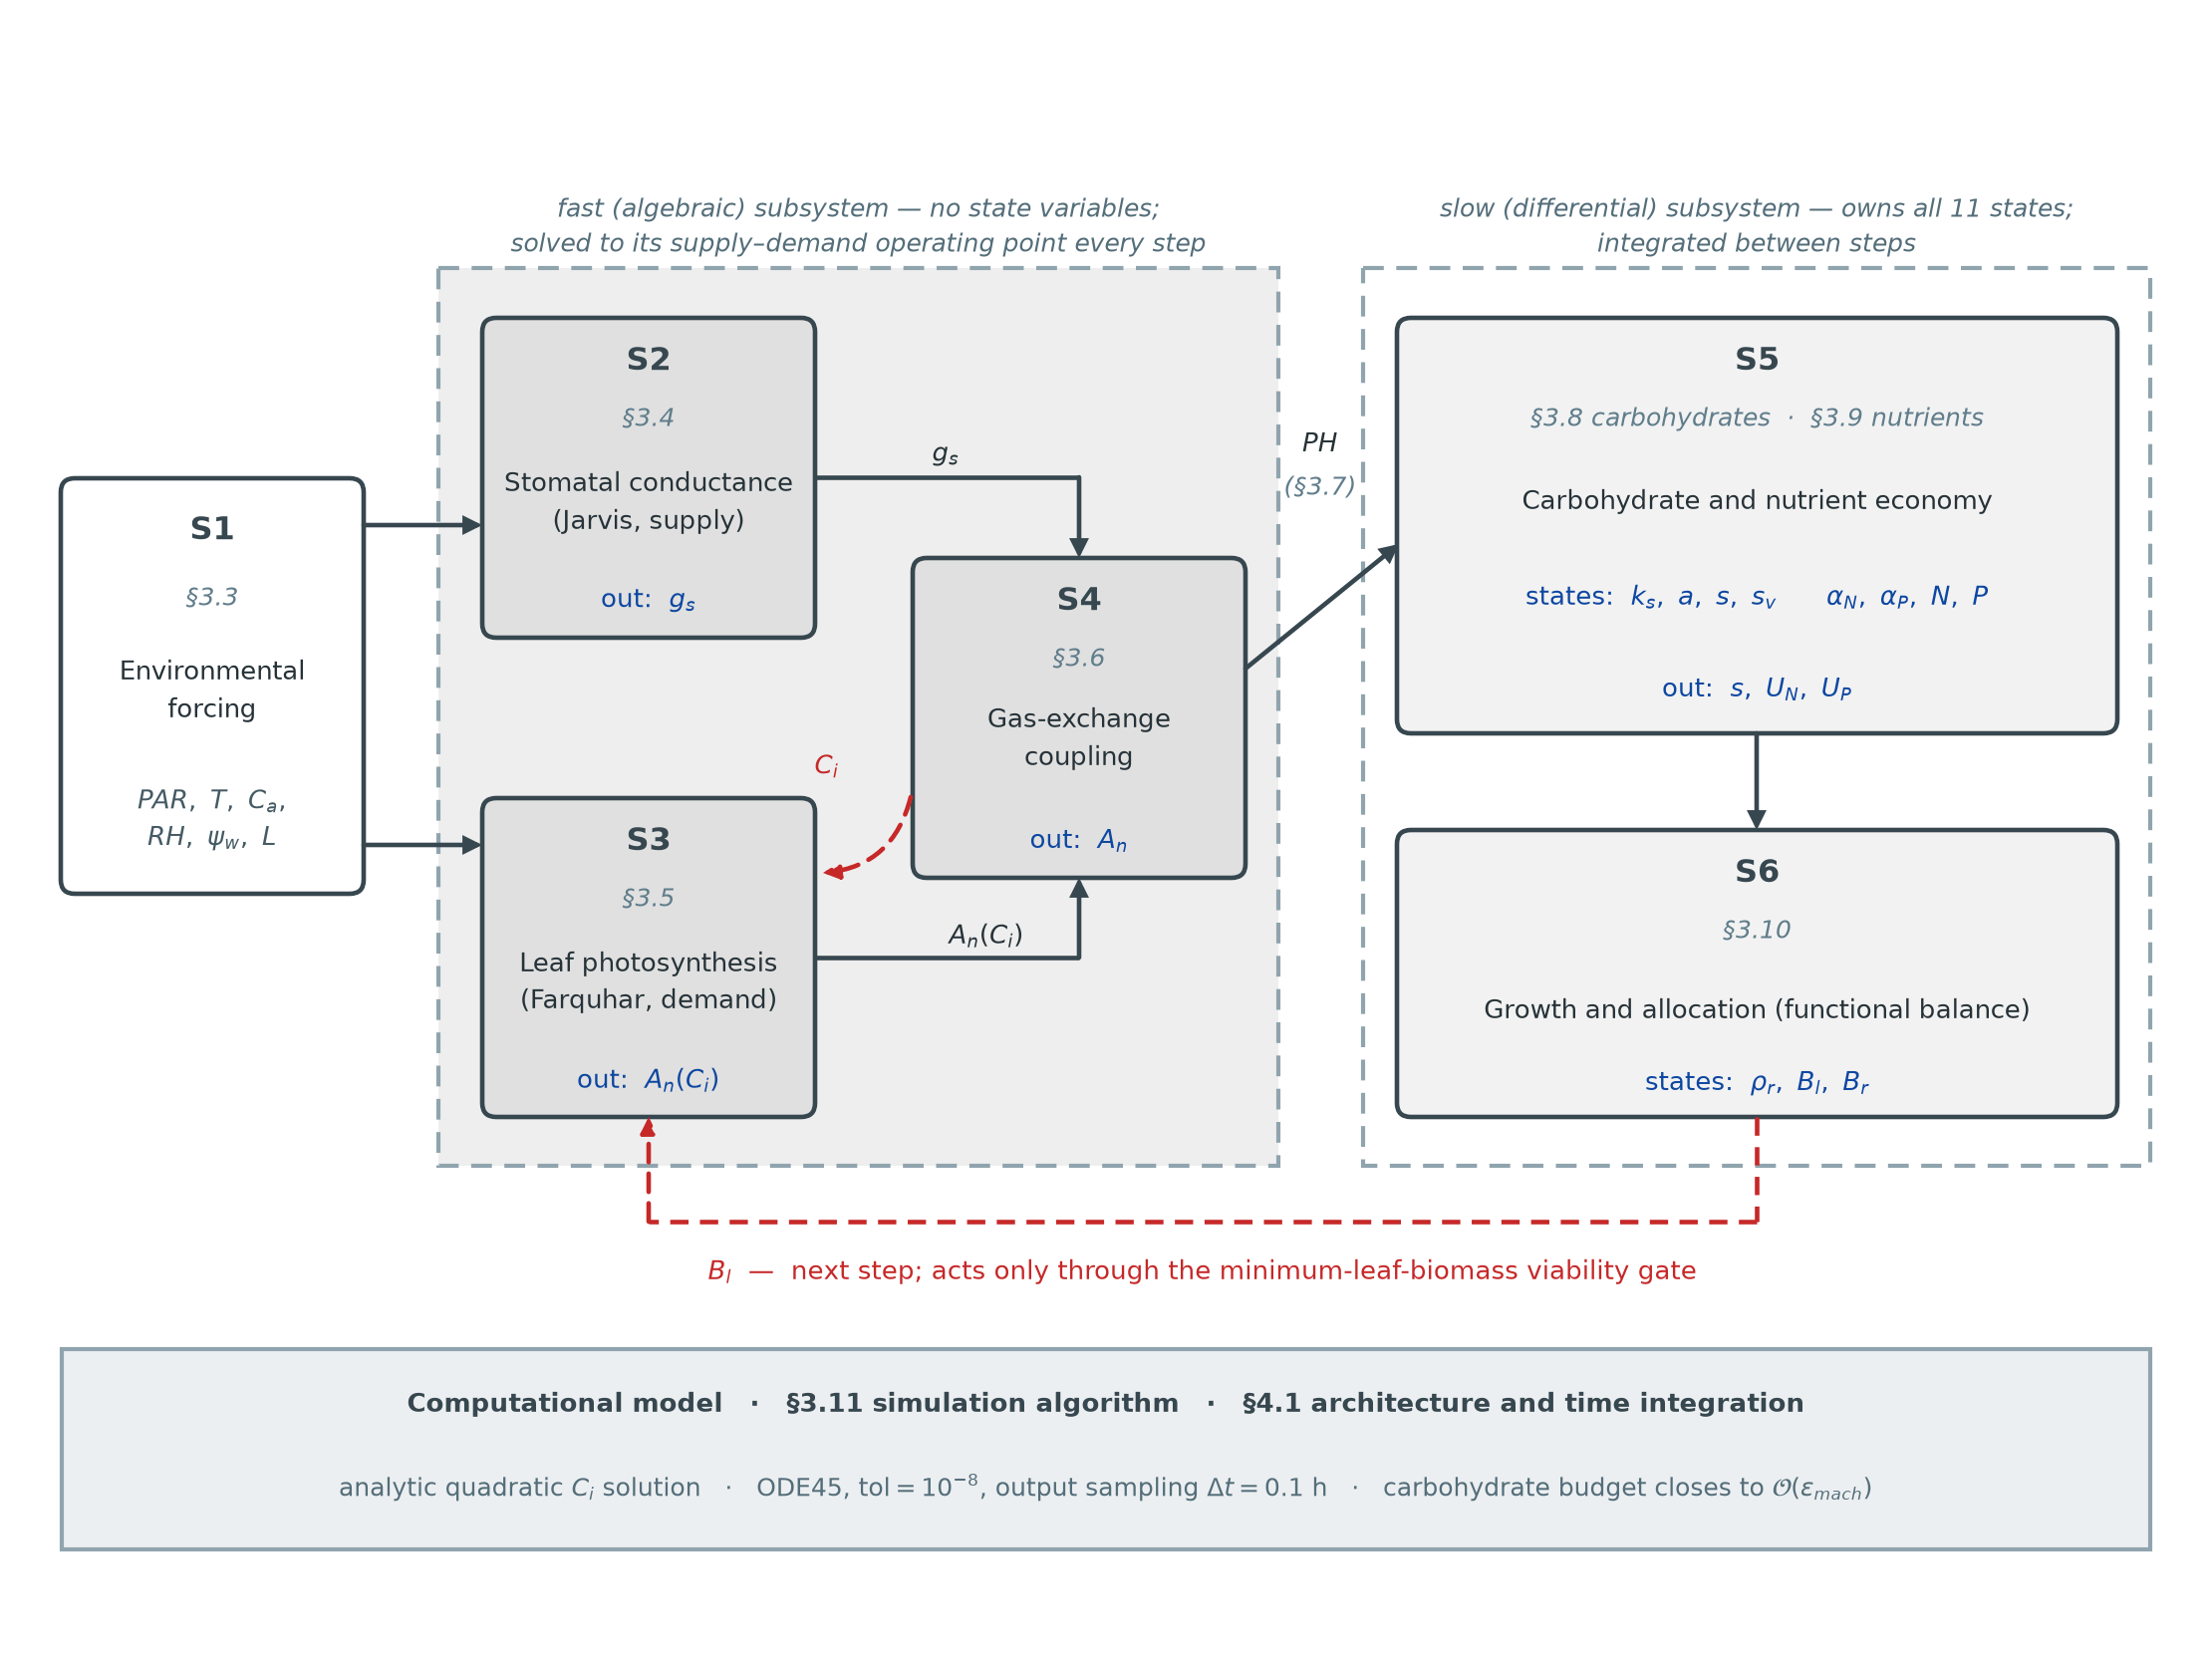
\includegraphics[width=\textwidth]{model_overview.png}
\caption{Structure of the model formulation and road map of
Section~\ref{sec:model}. Boxes are the six submodels S1--S6 of
Section~\ref{sec:conceptual}, annotated with the subsection in which each is
specified, the state variables it owns and the signals it exports. Solid
arrows carry fluxes and algebraic signals within a single derivative
evaluation. The single dashed return arrow carries leaf biomass $B_l$ from
S6 back to the gas-exchange layer, where it acts as a viability gate only
($\Phi_c = 0$ when $B_l < B_{l,\min}$; Eq.~\eqref{eq:conversion}): there is
no feedback of photosynthetic capacity in the model as implemented, and the
Farquhar capacities $V_{c\max}$ and $J_{\max}$ are fixed parameters
throughout. Background tint distinguishes the fast algebraic gas-exchange
subsystem S2--S4, whose supply-demand operating point is obtained in closed
form (Eq.~\eqref{eq:ci_quadratic}) at every derivative evaluation, from the
slow differential subsystem S5--S6; the two are labelled in the figure. The
slow states are advanced by an adaptive Dormand--Prince \texttt{ODE45}
embedded pair under local error control, not by a fixed-step scheme, so the
gas-exchange layer is re-evaluated at every Runge--Kutta stage rather than
once per step (Section~\ref{sec:algorithm}).
Figure~\ref{fig:blockdiagram} shows the same decomposition at the level of
individual interface signals.}
\label{fig:model_overview}
\end{figure*}

\subsection{Conceptual model and system decomposition}
\label{sec:conceptual}

The system studied is a single vegetative Arabidopsis plant together with
its immediate physical environment. The system boundary encloses the plant;
radiation, temperature, atmospheric humidity and CO$_2$, and soil water and
nutrient status cross the boundary as external inputs, while carbon and
nutrient acquisition, storage, and allocation to leaf and root biomass are
the internal states. The plant is represented as a two-compartment
(leaf/root) whole-organism system rather than a spatial one, so
that transport within the plant is represented by aggregate pools rather than
by explicit geometry. This lumped, functional-balance decomposition and the
underlying carbon-nutrient allocation states follow the whole-plant growth
framework of \citet{Tedone2020}, which the present work extends by replacing
the prescribed carbon input with a computed Farquhar-Jarvis gas-exchange
layer.

The system is decomposed into six submodels that exchange a small number of
defined signals (Fig.~\ref{fig:blockdiagram}; the block diagram is
described here in text and its interfaces are those listed below):

\begin{enumerate}\itemsep2pt
\item[\textbf{S1}] \emph{Environmental forcing} -- maps clock time to the
      photoperiod switch and the instantaneous radiation and micro-climate.
      \emph{In:} time $t$, scenario parameters. \emph{Out:}
      $\mathit{PAR},T,C_a,\mathit{RH},\psi_w,L$.
\item[\textbf{S2}] \emph{Stomatal conductance (supply)} -- the Jarvis
      multiplicative model. \emph{In:} $\mathit{PAR},T,C_a,\mathit{RH},
      \psi_w$. \emph{Out:} $g_s$.
\item[\textbf{S3}] \emph{Leaf photosynthesis (demand)} -- the Farquhar
      C$_3$ biochemical model. \emph{In:} $\mathit{PAR},C_i$, and the fixed
      capacity parameters $V_{c\max},J_{\max}$. \emph{Out:} $A_n(C_i)$.
\item[\textbf{S4}] \emph{Gas-exchange coupling} -- closes supply against
      demand for the operating point. \emph{In:} $g_s$, $A_n(C_i)$, $C_a$.
      \emph{Out:} $A_n$, and after scaling the carbon input $\Phi_c$.
\item[\textbf{S5}] \emph{Carbohydrate and nutrient economy} -- diel
      starch/sucrose partitioning and sucrose-limited N,\,P uptake.
      \emph{In:} $\Phi_c$, soil $N_s,P_s$. \emph{Out:} sucrose $s$, uptakes
      $U_N,U_P$.
\item[\textbf{S6}] \emph{Growth and allocation} -- converts sucrose into
      leaf and root biomass under functional-balance control. \emph{In:}
      $s,U_N,U_P$. \emph{Out:} $B_l,B_r$ and the allocation/investment
      states.
\end{enumerate}

\begin{figure}[!htbp]
\centering
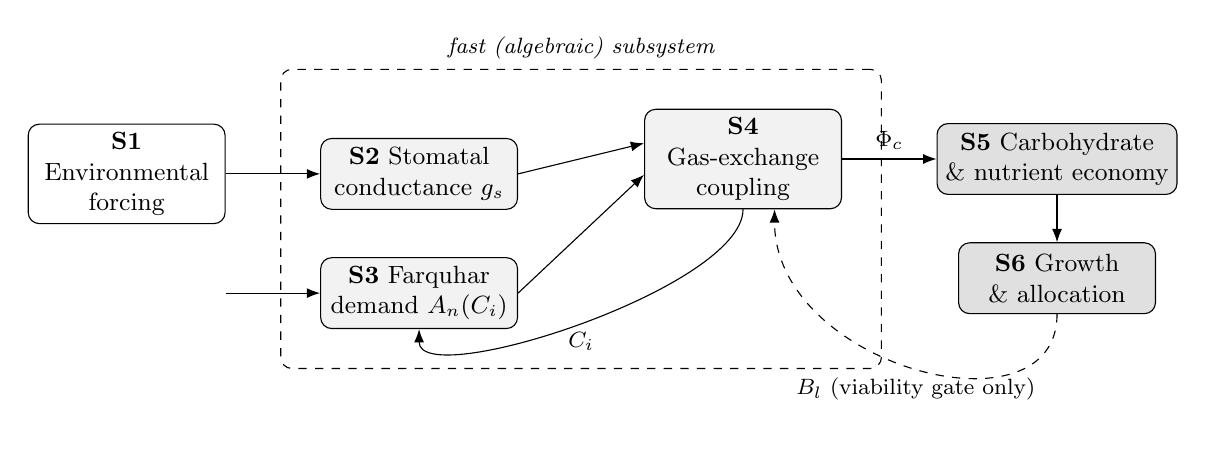
\begin{tikzpicture}[
  font=\small,
  box/.style={draw, rounded corners, minimum width=25mm, minimum height=9mm,
              align=center, inner sep=3pt},
  fast/.style={box, fill=black!5},
  slow/.style={box, fill=black!12},
  env/.style={box, fill=white},
  >=Latex, node distance=6mm and 12mm
]
% environment
\node[env] (m1) {\textbf{S1}\\Environmental\\forcing};
% fast subsystem
\node[fast, right=of m1] (m2) {\textbf{S2} Stomatal\\conductance $g_s$};
\node[fast, below=of m2] (m3) {\textbf{S3} Farquhar\\demand $A_n(C_i)$};
\node[fast, right=16mm of m2, yshift=-\the\dimexpr0.5\baselineskip-4mm\relax] (m4)
      {\textbf{S4}\\Gas-exchange\\coupling};
% slow subsystem
\node[slow, right=of m4] (m5) {\textbf{S5} Carbohydrate\\ \& nutrient economy};
\node[slow, below=of m5] (m6) {\textbf{S6} Growth\\ \& allocation};
% dashed grouping for fast subsystem
\begin{scope}[on background layer]
  \node[draw, dashed, rounded corners, fit=(m2)(m3)(m4),
        inner sep=5mm, label={[font=\footnotesize\itshape]above:fast (algebraic) subsystem}] {};
\end{scope}
% edges
\draw[->] (m1.east|-m2) -- (m2.west);
\draw[->] (m1.east|-m3) -- (m3.west);
\draw[->] (m2.east) -- ([yshift=2mm]m4.west);
\draw[->] (m3.east) -- ([yshift=-2mm]m4.west);
\draw[->] (m4.east) -- node[above,font=\footnotesize]{$\Phi_c$} (m5.west);
\draw[->] (m5.south) -- (m6.north);
% feedback C_i from S4 to S3
\draw[->] (m4.south) .. controls +(0,-10mm) and +(0,-8mm) ..
      node[below,font=\footnotesize]{$C_i$} (m3.south);
% feedback: leaf biomass acts only as a viability gate on the carbon input
\draw[->,dashed] (m6.south) .. controls +(0,-16mm) and +(0,-20mm) ..
      node[below,font=\footnotesize]{$B_l$ (viability gate only)}
      ([xshift=4mm]m4.south);
\end{tikzpicture}


\caption{Decomposition of the whole-plant model into six submodels and their
interface signals. S2--S4 form the fast algebraic gas-exchange subsystem
(dashed box), whose supply-demand operating point is obtained in closed form
at every derivative evaluation; its scaled output $\Phi_c$ drives the slow
carbohydrate/nutrient and growth states S5--S6. The only return path from the
slow to the fast subsystem is leaf biomass $B_l$, and it enters solely as the
viability gate on the carbon input (Eq.~\eqref{eq:conversion}); the
photosynthetic capacities are fixed parameters and are not fed back.}
\label{fig:blockdiagram}
\end{figure}

Submodels S2--S4 form a \emph{fast} algebraic subsystem: gas exchange
equilibrates on a timescale of seconds and is treated as instantaneously
relaxed relative to the \emph{slow} states in S5-S6, which evolve over the
day-night cycle. This fast-slow separation is exploited directly by the
numerical model of Section~\ref{sec:algorithm}, where the fast subsystem
enters as an algebraic constitutive layer inside the derivative of the slow
states, evaluated in closed form and therefore without an inner iteration
\citep{Cellier1991}.

The formulation rests on the following simplifying assumptions.
\begin{enumerate}\itemsep1pt
\item[(A1)] The plant is spatially lumped into leaf and root compartments;
      no within-organ gradients or explicit canopy architecture are
      resolved.
\item[(A2)] Leaf gas exchange is at steady state at every instant, so
      the intercellular CO$_2$ concentration is the algebraic supply-demand
      balance rather than a differential state (Section~\ref{sec:closure}).
\item[(A3)] Stomatal conductance responds to the environment
      multiplicatively and independently of the assimilation rate
      (Jarvis-Stewart closure), so the supply function contains no explicit
      feedback from $A_n$ \citep{Jarvis1976,Damour2010}.
\item[(A4)] Transitory starch is degraded at a near-constant nocturnal rate
      calibrated to be almost exhausted at dawn, consistent with the
      observed circadian control of starch turnover
      \citep{Graf2010,Scialdone2013}.
\item[(A5)] Active nutrient uptake is energetically limited by cytosolic
      sucrose, so carbon and nutrient acquisition are explicitly co-limiting
      \citep{Smith2007}.
\item[(A6)] Biomass partitioning between shoot and root follows
      functional-balance theory: investment shifts toward the resource that
      most limits growth \citep{Thornley1972,ThornleyJohnson1990}.
\end{enumerate}

\subsection{State-space representation}
\label{sec:state}

The model state is the vector $X(t)\in\mathbb{R}^{n}$, whose evolution is
governed by the ordinary differential system with fixed parameters

\begin{equation}
\frac{dX(t)}{dt} = f\!\left(X(t),\,U(t),\,\boldsymbol{\theta},\,t\right),
\label{eq:ode_general}
\end{equation}

where $U(t)$ is the exogenous environmental forcing, $\boldsymbol{\theta}$
is the time-invariant parameter set, and the time dependence
enters only through the diel forcing. The state vector comprises $n=11$
components,

\begin{equation}
X(t) =
\left[
k_s,\;
a,\;
s,\;
\alpha_N,\;
\alpha_P,\;
N,\;
P,\;
\rho_r,\;
B_l,\;
B_r,\;
s_v
\right]^{\mathsf{T}},
\label{eq:state_vector}
\end{equation}

with the following interpretation: $k_s$ is the starch partition
coefficient (dimensionless), i.e.\ the fraction of gross assimilate
directed to starch; $a$ is the transitory starch pool and $s$ the
cytosolic sucrose pool ($\mu\mathrm{mol\ gFW^{-1}}$); $\alpha_N,\alpha_P$
are the nitrogen and phosphorus investment (affinity) states; $N,P$ are the
internal nitrogen and phosphorus pools ($\mu\mathrm{mol\ gFW^{-1}}$);
$\rho_r$ is the
sucrose-to-root allocation state; $B_l,B_r$ are leaf and root biomass (gFW);
and $s_v$ is a vacuolar sucrose pool ($\mu\mathrm{mol\ gFW^{-1}}$) exchanging
with the cytosolic pool. All five pool states are specific quantities on a
whole-plant fresh-weight basis; Section~\ref{sec:carbohydrates} states
precisely what that basis is and what it implies for the balance equations.
The exogenous forcing is

\begin{equation}
U(t) =
\left[
\mathit{PAR}(t),\;
T(t),\;
C_a(t),\;
\mathit{RH}(t),\;
\mathit{VPD}(t),\;
\psi_w(t),\;
L(t)
\right]^{\mathsf{T}},
\label{eq:input_vector}
\end{equation}

collecting photosynthetically active radiation $\mathit{PAR}$
($\mu\mathrm{mol\ m^{-2}\ s^{-1}}$), leaf temperature $T$
($^\circ\mathrm{C}$), ambient CO$_2$ concentration $C_a$
($\mu\mathrm{mol\ mol^{-1}}$), relative humidity $\mathit{RH}$ (\%), vapour
pressure deficit $\mathit{VPD}$ (kPa), leaf water potential $\psi_w$
(MPa), and the binary photoperiod signal $L(t)$. As indicated in
Eqs.~\eqref{eq:vpd_es}-\eqref{eq:vpd_def}, $\mathit{VPD}$ is a diagnostic
function of $T$ and $\mathit{RH}$ and is therefore not an independent
forcing; it is listed in $U(t)$ because it enters the stomatal response
directly.

\subsection{Submodel S1: environmental forcing}
\label{sec:forcing}

Let $h(t)=t \bmod 24$ denote the hour of day and $f$ the photoperiod
length (h). The light/dark switch is

\begin{equation}
L(t) =
\begin{cases}
1, & 0 \leq h(t) < f, \\[2pt]
0, & f \leq h(t) < 24,
\end{cases}
\label{eq:photoperiod}
\end{equation}

and the incident radiation follows a half-sinusoidal daytime profile that is
zero at night,

\begin{equation}
\mathit{PAR}(t) =
\begin{cases}
\mathit{PAR}_{\max}\,
\sin\!\left(\pi\,\dfrac{h(t)}{f}\right), & 0 \leq h(t) < f, \\[8pt]
0, & f \leq h(t) < 24,
\end{cases}
\label{eq:par_profile}
\end{equation}

where $\mathit{PAR}_{\max}$ is the scenario-specific peak irradiance. The
sinusoidal envelope is a smooth idealisation of the daily light course
that reaches its maximum at solar noon ($h=f/2$); it is the driver of both
the demand (through electron transport, Eq.~\eqref{eq:J_nrh}) and the
supply (through the Jarvis light response, Eq.~\eqref{eq:jarvis_par}) side
of gas exchange, and thereby imposes the day-night rhythm on the entire system.

\subsection{Submodel S2: stomatal conductance (supply)}
\label{sec:jarvis}

This submodel takes the micro-climate from S1 and returns the stomatal
conductance $g_s$; it is the supply side of gas exchange and carries no
dependence on the assimilation rate (assumption~A3). Stomatal conductance
is represented by the multiplicative (Jarvis-Stewart) form
\citep{Jarvis1976,Damour2010}, in which a maximal conductance is reduced by
a product of independent, dimensionless environmental modifiers, each
bounded in $[0,1]$:

\begin{equation}
g_s =
g_{s,\max}\,
f_{\mathit{PAR}}(\mathit{PAR})\,
f_{\mathit{VPD}}(\mathit{VPD})\,
f_{T}(T)\,
f_{\mathit{CO_2}}(C_a)\,
f_{w}(\psi_w).
\label{eq:jarvis_general}
\end{equation}

The multiplicative closure assumes that the environmental controls act
independently and non-synergistically; it remains the most widely used
empirical conductance model and requires no iterative optimisation
\citep{Damour2010,Buckley2017}. The maximal conductance
$g_{s,\max}$ is carried as an explicit parameter separate from the shape
parameters of the modifiers. This separation is not cosmetic: it keeps the
magnitude of the conductance in one place, so that each $f_i$ can be
required to satisfy $f_i \in [0,1]$ with a value of unity at its own
non-limiting reference condition, and so that a correction to the shape of
one modifier does not silently rescale the whole conductance. The
individual response functions are specified as follows.

\paragraph{Light response.}
A saturating (rectangular-hyperbola) response with a small residual
(cuticular/night) conductance $b_{10}$,

\begin{equation}
f_{\mathit{PAR}}(\mathit{PAR}) =
\begin{cases}
b_{10}, & \mathit{PAR} \leq q, \\[4pt]
\dfrac{b_1 b_2 (\mathit{PAR}-q)}{\,b_1 + b_2 (\mathit{PAR}-q)\,}, & \mathit{PAR} > q,
\end{cases}
\qquad q=\frac{b_{10}}{b_1}.
\label{eq:jarvis_par}
\end{equation}

The two branches do not meet. With the values of
Table~\ref{tab:param_values} the breakpoint is
$q = b_{10}/b_1 = 0.0833\ \mu\mathrm{mol\ m^{-2}\ s^{-1}}$, where the first
branch gives $f_{\mathit{PAR}}=b_{10}=0.05$ and the second gives
$f_{\mathit{PAR}}\to 0$: the modifier drops by $b_{10}$ as $\mathit{PAR}$
crosses $q$ from below, and does not regain $0.05$ until
$\mathit{PAR} = 27.36\ \mu\mathrm{mol\ m^{-2}\ s^{-1}}$. The intent of the
construction is evidently a residual conductance floor,
$f_{\mathit{PAR}} = \max(b_{10},\,\text{hyperbola})$, which would place the
crossover at $27.36$ and be continuous there; the implemented form instead
switches at $q$ and is not. We report the behaviour as implemented, since it
is what produced every number in this paper, but the jump is a defect rather
than a modelling choice and the floor form is the appropriate correction.

Its practical consequence is small and bounded, for a reason worth stating
because it is not the reason one would guess. The interval affected,
$0.0833 < \mathit{PAR} < 27.36\ \mu\mathrm{mol\ m^{-2}\ s^{-1}}$, lies almost
entirely below the light compensation point of the gas-exchange system
($13.4\ \mu\mathrm{mol\ m^{-2}\ s^{-1}}$ at the default parameters, and
higher under the reduced conductance the jump itself produces), where the
carbon input is zero regardless of $g_s$. The discontinuity is therefore
mostly invisible in $\Phi_c$; where it is not, it acts by lowering conductance in
the first minutes after dawn and the last before dusk. It does, however,
remain a discontinuity in a quantity the integrator differences, and it is
one of the reasons the step-size controller contracts sharply at the
light--dark transitions (Section~\ref{sec:algorithm}). The half-sinusoidal
forcing of Eq.~\eqref{eq:par_profile} traverses this interval in $1.7$ to
$5.2$ minutes of simulated time at the four photoperiods studied here (rising
and again falling), which bounds the exposure.

\paragraph{Vapour-pressure-deficit response.}
A linear decline with atmospheric demand, floored at zero,

\begin{equation}
f_{\mathit{VPD}}(\mathit{VPD}) =
\max\!\left(0,\; 1 - b_5\,\mathit{VPD}\right).
\label{eq:jarvis_vpd}
\end{equation}

\paragraph{Temperature response.}
A skewed parabolic optimum \citep{Jarvis1976} defined between a lower limit
$T_1$ and an upper limit $T_h$ with optimum near $T_0$,

\begin{equation}
f_{T}(T) =
b_3\,(T - T_1)\,(T_h - T)^{b_4},
\qquad
b_4 = \frac{T_h - T_0}{T_0 - T_1},
\quad
b_3 = \frac{1}{(T_0 - T_1)\,(T_h - T_0)^{b_4}},
\label{eq:jarvis_T}
\end{equation}

so that $f_T(T_1)=f_T(T_h)=0$ and $f_T(T_0)=1$ with the maximum located
\emph{at} $T_0$; with $T_1=5$, $T_0=25$ and $T_h=45^{\circ}$C this gives
$b_4=1$ and a single-peaked curve requiring no clipping. Both constants
differ from those used in the originally submitted implementation, and
Section~\ref{sec:verification} documents the correction and its consequences.

\paragraph{CO$_2$ response.}
A piecewise-linear reduction of conductance with increasing ambient CO$_2$,

\begin{equation}
f_{\mathit{CO_2}}(C_a) =
\begin{cases}
1, & C_a < 100, \\[4pt]
1 - b_7\,(C_a - 100), & 100 \leq C_a < 1000, \\[4pt]
b_8, & C_a \geq 1000,
\end{cases}
\qquad
b_7 = \frac{1-b_8}{900},
\label{eq:jarvis_co2}
\end{equation}

with $C_a$ in $\mu\mathrm{mol\ mol^{-1}}$.

\paragraph{Water-status response.}
A saturating (exponential) recovery of conductance above a minimum leaf
water potential $\psi_{\min}$,

\begin{equation}
f_{w}(\psi_w) =
1 - \exp\!\left(-b_6\,(\psi_w - \psi_{\min})\right),
\label{eq:jarvis_water}
\end{equation}

clipped to $[0,1]$. The vapour pressure deficit driving
Eq.~\eqref{eq:jarvis_vpd} is obtained from leaf temperature and relative
humidity through the Tetens saturation relation \citep{Monteith1965,Nobel2009},

\begin{align}
e_s &= 0.61078\,\exp\!\left(\frac{17.27\,T}{T+237.3}\right),
\label{eq:vpd_es}\\[4pt]
e_a &= e_s\,\frac{\mathit{RH}}{100},
\label{eq:vpd_ea}\\[4pt]
\mathit{VPD} &= e_s - e_a,
\label{eq:vpd_def}
\end{align}

with $e_s,e_a,\mathit{VPD}$ in kPa. The Jarvis model thus returns an
environment-dependent conductance that modulates the CO$_2$ supply to the
mesophyll without any explicit dependence on the assimilation rate,
providing the supply constraint that is closed against the biochemical
demand in Section~\ref{sec:closure}.

\begin{table}[!htbp]
\centering
\small
\caption{Principal symbols. Rate/flux units for the carbohydrate pools are
$\mu\mathrm{mol\ gFW^{-1}\ h^{-1}}$; leaf-level assimilation is in
$\mu\mathrm{mol\ CO_2\ m^{-2}\ s^{-1}}$.}
\label{tab:symbols}
\begin{tabular}{@{}lll@{}}
\toprule
Symbol & Meaning & Units \\
\midrule
\multicolumn{3}{@{}l}{\emph{State variables} $X(t)$}\\
$k_s$          & Starch partition coefficient            & -- \\
$a$            & Transitory starch pool                  & $\mu\mathrm{mol\ gFW^{-1}}$ \\
$s$            & Cytosolic sucrose pool                  & $\mu\mathrm{mol\ gFW^{-1}}$ \\
$s_v$          & Vacuolar sucrose pool                   & $\mu\mathrm{mol\ gFW^{-1}}$ \\
$\alpha_N,\alpha_P$ & N, P investment (affinity) states  & -- \\
$N,P$          & Internal nitrogen, phosphorus content   & $\mu\mathrm{mol\ gFW^{-1}}$ \\
$\rho_r$       & Sucrose-to-root allocation state        & -- \\
$B_l,B_r$      & Leaf, root biomass                      & gFW \\
\midrule
\multicolumn{3}{@{}l}{\emph{Environmental forcing} $U(t)$}\\
$\mathit{PAR}$ & Photosynthetically active radiation     & $\mu\mathrm{mol\ m^{-2}\ s^{-1}}$ \\
$T$            & Leaf temperature                        & $^\circ\mathrm{C}$ \\
$C_a$          & Ambient CO$_2$ concentration            & $\mu\mathrm{mol\ mol^{-1}}$ \\
$\mathit{RH}$  & Relative humidity                       & \% \\
$\mathit{VPD}$ & Vapour pressure deficit                 & kPa \\
$\psi_w$       & Leaf water potential                    & MPa \\
$L$            & Photoperiod (light/dark) switch         & -- \\
\midrule
\multicolumn{3}{@{}l}{\emph{Gas exchange}}\\
$g_s,g_c$      & Stomatal conductance to H$_2$O, CO$_2$  & $\mathrm{mol\ m^{-2}\ s^{-1}}$ \\
$C_i$          & Intercellular CO$_2$ concentration      & $\mu\mathrm{mol\ mol^{-1}}$ \\
$A_c,A_j,A_n$  & Rubisco-, RuBP-limited, net assimilation& $\mu\mathrm{mol\ m^{-2}\ s^{-1}}$ \\
$V_{c\max}$    & Maximum carboxylation rate              & $\mu\mathrm{mol\ m^{-2}\ s^{-1}}$ \\
$J,J_{\max}$   & Actual, maximum electron transport rate & $\mu\mathrm{mol\ m^{-2}\ s^{-1}}$ \\
$\Gamma^{*}$   & CO$_2$ compensation point ($R_d=0$)     & $\mu\mathrm{mol\ mol^{-1}}$ \\
$K_c,K_o$      & Michaelis constants (CO$_2$, O$_2$)     & $\mu\mathrm{mol\ mol^{-1}}$; $\mathrm{mmol\ mol^{-1}}$ \\
$O$            & Oxygen concentration                    & $\mathrm{mmol\ mol^{-1}}$ \\
$R_d$          & Dark (day) respiration rate             & $\mu\mathrm{mol\ m^{-2}\ s^{-1}}$ \\
$\phi,\theta$  & Quantum yield, curvature (Eq.~\eqref{eq:J_root}) & --; -- \\
$\Phi_c$           & Whole-plant gross carbon input          & $\mu\mathrm{mol\ gFW^{-1}\ h^{-1}}$ \\
$\mathrm{SLA}$ & Specific leaf area                      & $\mathrm{m^2\ gFW^{-1}}$ \\
\midrule
\multicolumn{3}{@{}l}{\emph{Nutrients, growth, and parameters}}\\
$U_N^{\text{pot}},U_P^{\text{pot}}$ & Potential N, P uptake   & $\mu\mathrm{mol\ gFW^{-1}\ h^{-1}}$ \\
$U_N,U_P$      & Realised (sucrose-limited) N, P uptake  & $\mu\mathrm{mol\ gFW^{-1}\ h^{-1}}$ \\
$I_{N,\max},I_{P,\max}$ & Maximal uptake rates            & $\mu\mathrm{mol\ gFW^{-1}\ h^{-1}}$ \\
$K_N,K_P$      & Uptake half-saturation constants        & $\mu\mathrm{mol\ (soil)}$ \\
$c_N,c_P$      & Sucrose cost per unit N, P acquired     & $\mu\mathrm{mol}$ (sucrose) $\mu\mathrm{mol}^{-1}$ \\
$\tau$         & Reference time scale of the uptake limitation (Eqs.~\eqref{eq:UN}-\eqref{eq:UP}), $=1$~h & h \\
$D_a$          & Starch degradation flux                 & $\mu\mathrm{mol\ gFW^{-1}\ h^{-1}}$ \\
$\mu_l,\mu_r$  & Leaf, root mortality rates              & $\mathrm{h^{-1}}$ \\
$\gamma_l,\gamma_r$ & Self-competition coefficients      & $\mathrm{gFW^{-1}\ h^{-1}}$ \\
$\boldsymbol{\theta}$ & Time-invariant parameter set     & -- \\
$\epsilon$     & Numerical regularisation constant       & -- \\
\bottomrule
\end{tabular}
\end{table}

Table~\ref{tab:symbols} lists symbols and units. Because a reader
reproducing the model needs the numerical values as well, and needs to know
which of them were fitted, Table~\ref{tab:param_values} gives the complete
parameter set with nominal value, provenance and calibration status. Every
value is the one used in the reported runs, read from
\texttt{config/default.config} or from the source where a constant is
compiled in; the four coefficients marked as calibrated are the only fitted
quantities in the model.

\begin{table}[!htbp]
\centering
\scriptsize
\caption{Complete parameter set. ``Status'' distinguishes parameters fixed
from the literature or by construction (F) from the four calibrated
coefficients (C); ``Range'' gives the sensitivity-analysis interval where the
parameter was included in the global sensitivity design (see
Table~\ref{tab:sa_params} for sampling scales and per-parameter provenance).
Parameters compiled in as constants rather than exposed in the configuration
file are marked $\dagger$.}
\label{tab:param_values}
\begin{tabular}{@{}llllll@{}}
\toprule
Symbol & Meaning & Value & Units & St. & Range \\
\midrule
\multicolumn{6}{@{}l}{\emph{Jarvis stomatal response} (Eq.~\ref{eq:jarvis_general}), all $\dagger$}\\
$g_{s,\max}$ & Unstressed maximum conductance & $0.7071068$ & $\mathrm{mol\,m^{-2}\,s^{-1}}$ & F & -- \\
$b_1$        & PAR response asymptote          & $0.6$    & --   & F & -- \\
$b_2$        & PAR response initial slope      & $0.002$  & $\mathrm{m^{2}\,s\,\mu mol^{-1}}$ & F & -- \\
$b_{10}$     & PAR response floor              & $0.05$   & --   & F & -- \\
$q$          & PAR breakpoint, $b_{10}/b_1$    & $0.0833$ & $\mu\mathrm{mol\,m^{-2}\,s^{-1}}$ & F & -- \\
$b_5$        & VPD sensitivity                 & $0.2$    & $\mathrm{kPa^{-1}}$ & F & -- \\
$T_0$        & Temperature optimum             & $25$     & $^\circ\mathrm{C}$ & F & -- \\
$T_1,T_h$    & Lower, upper temperature zeros  & $5$, $45$ & $^\circ\mathrm{C}$ & F & -- \\
$b_4$        & $(T_h-T_0)/(T_0-T_1)$           & $1.0$    & --   & F & -- \\
$b_3$        & $1/((T_0-T_1)(T_h-T_0)^{b_4})$  & $2.5\times10^{-3}$ & -- & F & -- \\
$b_7,b_8$    & CO$_2$ response slope, floor    & $8.9\times10^{-4}$, $0.2$ & --  & F & -- \\
$b_6$        & Water-potential response rate   & $3.0$    & $\mathrm{MPa^{-1}}$ & F & -- \\
$\psi_{\min}$& Water potential at stomatal closure & $-1.5$ & MPa & F & -- \\
\midrule
\multicolumn{6}{@{}l}{\emph{Farquhar biochemistry} (Eqs.~\ref{eq:Ac}--\ref{eq:An}), all $\dagger$}\\
$V_{c\max}$  & Maximum carboxylation rate      & $45.0$  & $\mu\mathrm{mol\,m^{-2}\,s^{-1}}$ & F & $[20,120]$ \\
$J_{\max}$   & Maximum electron transport rate & $90.0$  & $\mu\mathrm{mol\,m^{-2}\,s^{-1}}$ & F & $[50,200]$ \\
$\Gamma^{*}$ & CO$_2$ compensation point       & $42.0$  & $\mu\mathrm{mol\,mol^{-1}}$ & F & -- \\
$K_c$        & Michaelis constant, CO$_2$      & $404.9$ & $\mu\mathrm{mol\,mol^{-1}}$ & F & -- \\
$K_o$        & Michaelis constant, O$_2$       & $278.4$ & $\mathrm{mmol\,mol^{-1}}$ & F & -- \\
$O$          & Oxygen concentration            & $210.0$ & $\mathrm{mmol\,mol^{-1}}$ & F & -- \\
$R_d$        & Day respiration rate            & $1.5$   & $\mu\mathrm{mol\,m^{-2}\,s^{-1}}$ & F & -- \\
$\phi$       & Quantum yield                   & $0.385$ & $\mathrm{mol\,mol^{-1}}$ & F & -- \\
$\theta$     & Curvature of the $J$ response   & $0.7$   & --   & F & -- \\
\midrule
\multicolumn{6}{@{}l}{\emph{Carbon-input conversion} (Eqs.~\ref{eq:conversion}--\ref{eq:kappa_prime})}\\
$\kappa'$    & Carbon-input coefficient        & $1.222\times10^{-2}$ & -- & C$^{\dagger}$ & -- \\
$\mathrm{SLA}$ & Specific leaf area            & $0.025$ & $\mathrm{m^{2}\,gFW^{-1}}$ & F & -- \\
$B_{l,\min}$ & Leaf-biomass viability floor    & $0.001$ & gFW  & F & -- \\
$\Phi_{c,\max}$  & Prescribed max.\ rate (M0 only) & $12.7$  & $\mu\mathrm{mol\,gFW^{-1}\,h^{-1}}$ & F & -- \\
\midrule
\multicolumn{6}{@{}l}{\emph{Carbohydrate dynamics}}\\
$\lambda_{sdi}$ & Daytime starch synthesis rate & $0.05$  & $\mathrm{h^{-1}}$ & C & -- \\
$\lambda_{sdr}$ & Starch degradation rate coeff.& $0.25$  & $\mathrm{h^{-1}}$ & F & -- \\
$\lambda_{sni}$ & Nocturnal starch partition    & \multicolumn{2}{l}{$0.16/0.15/0.13/0.08$ (4/6/8/12 h)} & F & excl. \\
$\lambda_{c}$   & Starch feedback coefficient   & \multicolumn{2}{l}{$0.82/0.79/0.67/0.62$ (4/6/8/12 h)} & F & -- \\
$\lambda_{g}$   & Night-efficiency coefficient  & $0.65$  & --   & F & -- \\
$k_s^{0}$       & Initial starch partition      & $0.6$   & --   & F & -- \\
$D_{a,\max}$    & Max.\ starch degradation rate & $6.0$   & $\mu\mathrm{mol\,gFW^{-1}\,h^{-1}}$ & F & -- \\
$s_{\max}$      & Sucrose reference scale       & $2.0$   & $\mu\mathrm{mol\,gFW^{-1}}$ & F & -- \\
$k_{in}$        & Cytosol-to-vacuole rate       & $0.10$  & $\mathrm{h^{-1}}$ & F & $[0.005,0.40]$ \\
$k_{out}$       & Vacuole-to-cytosol rate       & $0.08$  & $\mathrm{h^{-1}}$ & F & -- \\
$r_m$           & Maintenance respiration freq. & $0.79$  & $\mathrm{h^{-1}}$ & F & -- \\
$\phi_{load}$   & Sucrose loading frequency     & $1.98$  & $\mathrm{h^{-1}}$ & F & -- \\
$c_{tr}$        & Sucrose cost of transport     & $0.0035$& --   & F & -- \\
\midrule
\multicolumn{6}{@{}l}{\emph{Nutrients and growth}}\\
$\lambda_{sb}$  & Growth-rate coefficient       & \multicolumn{2}{l}{calibrated per photoperiod, $\approx3.8$--$5.9\times10^{-3}$} & C & -- \\
$I_{N,\max}$    & Maximal N uptake rate         & \multicolumn{2}{l}{see Table~\ref{tab:sa_params}} & F & incl. \\
$I_{P,\max}$    & Maximal P uptake rate         & \multicolumn{2}{l}{see Table~\ref{tab:sa_params}} & F & incl. \\
$\lambda_{csn}$ & Sucrose cost of N assimilation& $0.0267$& --   & F & -- \\
$\lambda_{k}$   & Uptake half-saturation scale  & $50.0$  & $\mu\mathrm{mol}$ & F & -- \\
$r^{*}$         & Optimal N:P stoichiometry     & $10.0$  & $\mathrm{mol\,mol^{-1}}$ & F & -- \\
$\rho_r^{0}$    & Initial root allocation       & $0.5$   & --   & F & -- \\
$\mu_l,\mu_r$   & Leaf, root mortality rates    & $5\times10^{-7}$ & $\mathrm{h^{-1}}$ & F & -- \\
$\gamma_l,\gamma_r$ & Self-competition coeff.   & $5\times10^{-7}$ & $\mathrm{gFW^{-1}\,h^{-1}}$ & F & -- \\
$B_l(0),B_r(0)$ & Initial leaf, root biomass    & $0.02$, $0.02$ & gFW & F & incl. \\
\bottomrule
\end{tabular}
\end{table}

\subsection{Submodel S3: leaf photosynthesis (demand)}
\label{sec:farquhar}

This submodel returns the net assimilation $A_n$ as a function of the
intercellular CO$_2$ concentration $C_i$; it is the demand side of gas
exchange and is closed against the S2 supply in Section~\ref{sec:closure}.
Gross CO$_2$ demand follows the Farquhar-von~Caemmerer-Berry biochemical
model \citep{Farquhar1980,vonCaemmerer2000}, in which assimilation is the
minimum of a Rubisco-limited and an electron-transport-limited (RuBP
regeneration) rate. The Rubisco-limited rate is

\begin{equation}
A_c =
V_{c\max}\,
\frac{C_i - \Gamma^{*}}
{C_i + K_c\!\left(1 + O/K_o\right)},
\label{eq:Ac}
\end{equation}

where $C_i$ is the intercellular CO$_2$ concentration, $\Gamma^{*}$ the
CO$_2$ compensation point in the absence of dark respiration, $V_{c\max}$
the maximum carboxylation rate, $K_c$ and $K_o$ the Michaelis constants of
Rubisco for CO$_2$ and O$_2$, and $O$ the oxygen concentration. The
electron-transport-limited rate is

\begin{equation}
A_j =
J\,
\frac{C_i - \Gamma^{*}}
{4.5\,C_i + 10.5\,\Gamma^{*}},
\label{eq:Aj}
\end{equation}

in which the denominator coefficients $\{4.5,\,10.5\}$ encode the electron
requirement per carboxylation and per oxygenation under the standard
stoichiometry of RuBP regeneration \citep{vonCaemmerer1981,vonCaemmerer2000}.
Net assimilation is the limiting process less dark respiration $R_d$,

\begin{equation}
A_n = \min(A_c,\,A_j) - R_d.
\label{eq:An}
\end{equation}

The potential electron transport rate $J$ is obtained from $\mathit{PAR}$
through the non-rectangular hyperbola \citep{Farquhar1980,Farquhar1984},

\begin{equation}
\theta\,J^{2} - \left(J_{\max} + \phi\,\mathit{PAR}\right) J
+ J_{\max}\,\phi\,\mathit{PAR} = 0,
\label{eq:J_nrh}
\end{equation}

whose lower root is taken,

\begin{equation}
J =
\frac{\left(J_{\max}+\phi\,\mathit{PAR}\right)
- \sqrt{\left(J_{\max}+\phi\,\mathit{PAR}\right)^{2}
- 4\,\theta\,J_{\max}\,\phi\,\mathit{PAR}}}
{2\,\theta},
\label{eq:J_root}
\end{equation}

with $\phi$ the apparent quantum yield for electron transport (including
leaf absorptance) and $\theta$ the curvature of the light response.

The submodel is evaluated whenever $\mathit{PAR}>0$ and leaf biomass exceeds
the viability minimum $B_{l,\min}$; in darkness, or below that biomass, the
carbon input is set to zero. No irradiance threshold is applied. The
originally submitted version of the model treated the leaf as
non-assimilating below $\mathit{PAR} = 20\ \mu\mathrm{mol\ m^{-2}\ s^{-1}}$,
which was removed for two reasons. First, it was a discontinuity in the
carbon input at a point every diel trajectory crosses twice a day: the
light modifier at that irradiance is $f_{\mathit{PAR}}(20)=0.0374 \neq 0$, so
the assimilation rate jumped rather than passing through the threshold, which
is a hazard for the error-controlled integrator of
Section~\ref{sec:algorithm}. Second, it is unnecessary: with the closed-form
operating point of Section~\ref{sec:closure} the net rate passes smoothly
through zero at the light compensation point --- $\mathit{PAR} = 13.4\
\mu\mathrm{mol\ m^{-2}\ s^{-1}}$ under the default parameterisation --- and
the terminal $\max(0,\cdot)$ applied to the carbon input returns exactly zero
below it, continuously and without a special case. Sub-compensation
irradiance is therefore handled by the physics rather than by a gate. Note
that $A_n$ itself remains negative there, and it is the whole-plant carbon
input, not $A_n$, that is clamped; the respiratory efflux is not treated as
an assimilatory gain.

\subsection{Submodel S4: gas-exchange coupling}
\label{sec:closure}

Equations~\eqref{eq:Ac}-\eqref{eq:An} express biochemical
\emph{demand} as a function of the intercellular CO$_2$ that is itself set,
through Fickian \emph{supply}, by the diffusion of CO$_2$ across the
stomata:

\begin{equation}
C_i = C_a - \frac{A_n}{g_c},
\qquad
g_c = \frac{g_s}{1.6},
\label{eq:diffusion}
\end{equation}

where the factor $1.6$ converts the water-vapour conductance $g_s$ to a
CO$_2$ conductance $g_c$, reflecting the lower molecular diffusivity of
CO$_2$ in air \citep{vonCaemmerer2000,Nobel2009}. Because $A_n$ depends on
$C_i$ and $C_i$ depends on $A_n$, the operating point is the mutual
solution of Eqs.~\eqref{eq:An} and~\eqref{eq:diffusion}. We obtain it by
fixed-point iteration \citep{Press2007}: starting from
$C_i^{(0)}=\eta\,C_a$ with $\eta=0.7$, the demand
Eqs.~\eqref{eq:Ac}-\eqref{eq:An} are evaluated at the current $C_i^{(k)}$,
the supply Eq.~\eqref{eq:diffusion} returns an updated
$C_i^{(k+1)}=\max\!\left(0,\;C_a - A_n^{(k)}/g_c\right)$, and the iteration
proceeds until both the concentration and the assimilation rate are
stable,

\begin{equation}
\left|C_i^{(k+1)} - C_i^{(k)}\right| < \varepsilon
\quad\text{and}\quad
\left|A_n^{(k)} - A_n^{(k-1)}\right| < \varepsilon,
\label{eq:convergence}
\end{equation}

with separate tolerances $\varepsilon_{C_i}$ and $\varepsilon_{A_n}$ for the
two criteria --- the two residuals have different dimensions and differ by
more than an order of magnitude in typical size, so a single absolute
tolerance is not defensible --- and an iteration cap $k_{\max}$. The
conductance $g_s$ is held fixed at its Jarvis value
(Eq.~\eqref{eq:jarvis_general}) during the inner iteration, so the
procedure resolves a genuine runtime coupling between the Jarvis supply
function and the Farquhar demand function at every time step. The scheme is
summarised in Algorithm~\ref{alg:ci_fixedpoint}.

The coupled system does not, however, require iteration at all, and the
production simulator does not use it. Substituting the supply relation
Eq.~\eqref{eq:diffusion} into either Farquhar branch yields a
\emph{quadratic} in $C_i$ that can be solved in closed form. Writing each
branch of Eqs.~\eqref{eq:Ac}-\eqref{eq:Aj} as a rational function
$A = \alpha(C_i-\Gamma^{*})/(C_i + \beta)$ --- with
$(\alpha,\beta) = \bigl(V_{c\max},\,K_c(1+O/K_o)\bigr)$ for the
Rubisco-limited branch and
$(\alpha,\beta) = \bigl(J/4.5,\;(10.5/4.5)\,\Gamma^{*}\bigr)$ for the
electron-transport-limited branch --- and equating supply and demand,
$g_c(C_a - C_i) = \alpha(C_i-\Gamma^{*})/(C_i+\beta) - R_d$, gives

\begin{equation}
g_c\,C_i^{2}
+ \bigl[\alpha - R_d + g_c(\beta - C_a)\bigr] C_i
- \bigl[\alpha\Gamma^{*} + R_d\,\beta + g_c\,C_a\,\beta\bigr] = 0,
\label{eq:ci_quadratic}
\end{equation}

whose physically admissible root is the larger one, since the product of the
roots is negative and exactly one root is positive. The operating point is
the branch-wise solution with the smaller assimilation rate, consistent with
the $\min(A_c,A_j)$ co-limitation of Eq.~\eqref{eq:An}. The sign of $R_d$ in
the linear coefficient is worth stating explicitly, because the originally
submitted manuscript printed it as $+R_d$. That was a transcription error in
the manuscript only: the implementation has always formed the coefficient as
$\alpha - R_d + g_c(\beta - C_a)$ --- in the source, as
$g_c(d_1C_a-d_0)-\alpha_{\text{num}}+R_d d_1$ with the leading coefficient
$-g_c d_1$, which is the same quadratic multiplied by $-1$ --- so every
number reported in this paper and in the earlier submission was computed from
the correct expression. We record the correction here rather than silently
amending the equation, since a reader checking the algebra against the code
would otherwise find a discrepancy that does not exist. We thank the reviewer
who caught it.

The admissibility rule applied to the two roots is $C_i \ge 0$ alone. A root
exceeding the ambient concentration is retained rather than rejected: by
Eq.~\eqref{eq:diffusion}, $C_i > C_a$ is exactly what the supply relation
returns whenever $A_n < 0$, that is, whenever the leaf is a net source below
the light compensation point, and it is physically correct there.

When the conductance vanishes the quadratic degenerates and no operating
point exists, so the implementation applies a boundary condition rather than
solving: for $g_c \le 0$ it sets

\begin{equation}
C_i = \Gamma^{*},
\qquad
A_n = -R_d,
\label{eq:ci_closed}
\end{equation}

that is, a genuine efflux of respiratory CO$_2$ and not zero assimilation.
Equation~\eqref{eq:ci_closed} is a stated convention of the implementation at
the boundary of the admissible conductance range, not the $g_s \to 0$ limit of
the coupled system; the limit itself is approached from the interior and is
not evaluated. We flag the distinction because a boundary convention and a
limit are different objects, and only the former is what the code executes.
Equation~\eqref{eq:ci_quadratic} is the default solver in all results
reported here. The iterative scheme of Eq.~\eqref{eq:convergence} and
Algorithm~\ref{alg:ci_fixedpoint} is retained behind a run-time switch, and
is used in Section~\ref{sec:verification} to characterise its own failure
modes against the closed form; presenting both is what makes that
verification possible.

\begin{algorithm}[!htbp]
\caption{Farquhar-Jarvis gas-exchange coupling: fixed-point solution of the intercellular CO$_2$ concentration.}
\label{alg:ci_fixedpoint}
\begin{algorithmic}[1]
\REQUIRE $C_a$, $g_s$, $\Gamma^{*}$, $V_{c\max}$, $K_c$, $K_o$, $O$, $J$, $R_d$; tolerance $\varepsilon$, cap $k_{\max}$
\ENSURE $A_n$, converged $C_i$
\STATE $C_i \leftarrow 0.7\,C_a$
\STATE $g_c \leftarrow g_s/1.6$;\quad $A_n^{\text{prev}} \leftarrow 0$
\FOR{$k \leftarrow 1$ \TO $k_{\max}$}
  \STATE $A_c \leftarrow V_{c\max}\,(C_i-\Gamma^{*}) / \bigl(C_i + K_c(1+O/K_o)\bigr)$
  \STATE $A_j \leftarrow J\,(C_i-\Gamma^{*}) / (4.5\,C_i + 10.5\,\Gamma^{*})$
  \STATE $A_n \leftarrow \min(A_c,A_j) - R_d$
  \STATE $C_i^{\text{new}} \leftarrow \max\!\bigl(0,\; C_a - A_n/g_c\bigr)$
  \IF{$|C_i^{\text{new}}-C_i| < \varepsilon$ \textbf{and} $|A_n - A_n^{\text{prev}}| < \varepsilon$}
    \STATE \textbf{break}
  \ENDIF
  \STATE $C_i \leftarrow C_i^{\text{new}}$;\quad $A_n^{\text{prev}} \leftarrow A_n$
\ENDFOR
\RETURN $A_n,\ C_i$
\end{algorithmic}
\end{algorithm}

\subsection{Conversion from assimilation to model carbon input}
\label{sec:conversion}

The leaf-level net assimilation $A_n$
($\mu\mathrm{mol\ CO_2\ m^{-2}\ s^{-1}}$) is converted to the
whole-plant gross carbon input $\Phi_c$ that drives the carbohydrate pools
($\mu\mathrm{mol\ gFW^{-1}\ h^{-1}}$):

\begin{equation}
\Phi_c =
\underbrace{\kappa'}_{\text{dimensionless}}\;
\underbrace{3600}_{\mathrm{s\,h^{-1}}}\;
\underbrace{\mathrm{SLA}}_{\mathrm{m^{2}\,gFW^{-1}}}\;
\underbrace{A_n}_{\mathrm{\mu mol\,m^{-2}\,s^{-1}}},
\qquad L(t)=1,
\label{eq:conversion}
\end{equation}

where $\mathrm{SLA}$ is the specific leaf area and the two explicit factors
carry the entire unit conversion: $\mathrm{SLA}$ converts the per-area flux
to a per-gram-fresh-weight basis and the factor $3600\ \mathrm{s\,h^{-1}}$
converts seconds to hours, so that $\Phi_c$ is in
$\mu\mathrm{mol\ gFW^{-1}\ h^{-1}}$ as stated. Only $\kappa'$ is
dimensionless, and it is a calibration coefficient, not a unit factor. The
earlier submission wrote this relation as
$\Phi_c=\kappa A_n\,\mathrm{SLA}/\mathrm{SLA}_{\text{ref}}$ with a
dimensionless $\kappa$ said to absorb the unit conversion. That form is
dimensionally inconsistent, as a dimensionless coefficient cannot convert
$\mathrm{m^{-2}\,s^{-1}}$ into $\mathrm{gFW^{-1}\,h^{-1}}$; we thank the
reviewer for identifying it. The implementation is unchanged --- it applies
a single constant $1.10$ at the reference $\mathrm{SLA}$ of
$0.025\ \mathrm{m^{2}\,gFW^{-1}}$ --- so the two forms agree numerically
with
\begin{equation}
\kappa' = \frac{1.10}{3600\,\mathrm{SLA}_{\text{ref}}}
        = \frac{1.10}{90} = 1.222\times10^{-2}.
\label{eq:kappa_prime}
\end{equation}
Writing the conversion this way makes the size of the fitted coefficient
visible: the coupled model retains about $1.2\%$ of the gross per-area
assimilation as carbon entering the whole-plant carbohydrate pools. That is
not a small correction to a physical conversion but the dominant empirical
scaling in the carbon-input pathway, and it is reported here as such rather
than concealed inside a symbol described as a unit factor. Its magnitude is
consistent with the model's treatment of $A_n$ as an upper-canopy,
light-saturated leaf rate while $\Phi_c$ is a whole-rosette average over
self-shaded leaves of mixed age, but the coefficient is calibrated, not
derived, and $\kappa'$ is therefore listed as a fitted parameter in
Table~\ref{tab:symbols}. Leaf biomass $B_l$ enters this
conversion only through the on/off viability guard
($\Phi_c=0$ when $B_l<B_{l,\min}$) and not as a continuous multiplier. In
darkness there is no gross fixation,

\begin{equation}
\Phi_c = 0, \qquad L(t)=0.
\label{eq:PH_night}
\end{equation}

\subsection{Submodel S5: carbohydrate and nutrient economy}
\label{sec:carbohydrates}

Before the balance equations, the meaning of the pool states must be fixed
precisely, because the units $\mu\mathrm{mol\ gFW^{-1}}$ admit two readings
that lead to different equations. The states $a$, $s$, $s_v$ (and likewise
$N$, $P$) are \emph{specific} pools: amount of substance per unit of
whole-plant fresh weight, i.e.\ intensive quantities, not extensive contents
of the growing plant. They are stated per gram of fresh weight so that
$\Phi_c$, which Eq.~\eqref{eq:conversion} delivers on the same basis, can
drive them directly without carrying $B_l+B_r$ through the carbohydrate
subsystem.

One consequence must be stated explicitly. For an intensive quantity in a
growing system, the material balance carries a dilution term: if $A$ is the
extensive amount and $B=B_l+B_r$ the fresh weight, then $a = A/B$ obeys
\begin{equation}
\frac{da}{dt}
= \frac{1}{B}\frac{dA}{dt} - \frac{a}{B}\frac{dB}{dt},
\label{eq:dilution}
\end{equation}
and the second term --- growth dilution --- is \emph{not} present in
Eqs.~\eqref{eq:starch}, \eqref{eq:sucrose} or~\eqref{eq:sucrose_vac}, nor in
Eqs.~\eqref{eq:dN}-\eqref{eq:dP}. The pool equations as implemented are
therefore per-gram balances of the fluxes only, and are exact for an
intensive pool only in the limit $B^{-1}\,dB/dt \to 0$. Over the horizons
simulated here that relative growth rate is $0.069$ to $0.261\
\mathrm{d^{-1}}$, i.e.\ $2.9\times10^{-3}$ to $1.1\times10^{-2}\ \mathrm{h^{-1}}$,
against diel turnover of the sucrose pool on the order of
$10^{-1}\ \mathrm{h^{-1}}$; the omitted term is thus one to two orders of
magnitude below the retained ones, which is why the diel trajectories are
qualitatively unaffected. It is not, however, negligible in the sense of
being absent from the model's intent: the calibrated coefficients
$\lambda_{sb}$ and $\lambda_{sdi}$ absorb its time-averaged effect, which is
one more reason the calibration residuals of Section~\ref{sec:results} cannot
be read as predictive errors. We flag this as a formulation limitation rather
than correct it here, since correcting it would change every calibrated value
in the paper.

The alternative reading --- that the pools are normalised state variables on
a nominal per-gram basis, with no claim to be concentrations of a growing
body --- is self-consistent and requires no dilution term. It is the reading
under which the implementation is correct as written, and it is the one we
adopt. What it costs is the direct interpretation of $a$ and $s$ as
measurable tissue concentrations: the comparison against measured
carbohydrate contents in Section~\ref{sec:results} is then a comparison of
shape and timing, and the absolute levels carry the calibration in them. The
figures are read that way throughout.

Fixed carbon is partitioned between transitory starch and cytosolic
sucrose. The starch pool accumulates a fraction $k_s$ of the carbon input
during the day and is remobilised at night,

\begin{equation}
\frac{da}{dt} = k_s\,\Phi_c - D_a,
\label{eq:starch}
\end{equation}

where $D_a$ is the starch degradation flux. Consistent with the
experimental observation that transitory starch is degraded at an
approximately constant rate calibrated to be nearly exhausted at dawn
\citep{Graf2010,Scialdone2013,Stitt2012}, $D_a$ is active only in
darkness ($L=0$) and is scaled by the remaining reserve and the time left
until dawn. Explicitly, with $a^{\dagger}$ the starch content latched at
the onset of darkness, $t_d = \mathrm{mod}(t,24)$ the hour of day and
$\Delta_n = 24 - P$ the night length,

\begin{equation}
D_a =
\begin{cases}
0, & a^{\dagger} < a_{\min},\\[6pt]
(1-L)\,
\min\!\left(
D_{a,\max},\;
\left[
\dfrac{t_d}{24}
+ \left(1-\dfrac{t_d}{24}\right)
\left(1 - \dfrac{s}{s+s_{\max}}\right)
\right]
\dfrac{a^{\dagger}-a_{\min}}{\Delta_n}
\right),
& a^{\dagger} \ge a_{\min},
\end{cases}
\label{eq:starch_degradation}
\end{equation}

where $D_{a,\max}$ caps the instantaneous mobilisation rate. The first
branch is a guard rather than a modelling choice: if the reserve latched at
dusk already lies below the residual pool $a_{\min}$ there is nothing
mobilisable, and prescribing a positive flux would drive the starch state
negative. The bracket interpolates between a purely clock-driven rate and a
sucrose-status-driven one, so that mobilisation accelerates when cytosolic
sucrose is depleted, and the divisor $\Delta_n$ paces the reserve to be
almost exhausted at dawn. Because $a^{\dagger}$ is held constant through
the night, $D_a$ has no explicit dependence on the current starch state $a$
during a night, which is what makes the near-linear nocturnal decline
observed by \citet{Graf2010} an emergent rather than an imposed property.
The cytosolic sucrose pool receives the complementary fraction
of the carbon input plus the starch-derived carbon, and is drained by
nutrient-uptake, transport, respiration, and phloem-loading costs, and by
net exchange with the vacuole:

\begin{equation}
\frac{ds}{dt} =
(1-k_s)\,\Phi_c + D_a
- C_{\text{uptake}}
- C_{\text{transport}}
- C_{\text{resp}}
- C_{\text{load}}
- k_{\text{in}}\,s + k_{\text{out}}\,s_v,
\label{eq:sucrose}
\end{equation}

\begin{equation}
\frac{ds_v}{dt} =
k_{\text{in}}\,s - k_{\text{out}}\,s_v.
\label{eq:sucrose_vac}
\end{equation}

The four sink terms in Eq.~\eqref{eq:sucrose} were not defined in the
original formulation and are given here in full. Respiration is
first-order in the cytosolic pool, and phloem loading is proportional to a
night-efficiency factor $E_{\text{night}}$ that represents the fraction of
mobile sucrose usable for export under the current light and partitioning
state:

\begin{align}
C_{\text{resp}} &= \phi_r\,s,
\label{eq:C_resp}\\[4pt]
C_{\text{load}} &= \phi_{\text{load}}\,E_{\text{night}},
\label{eq:C_load}\\[4pt]
E_{\text{night}} &=
\min(s,s_{\max})\,
\Bigl[
\lambda_g + (1-\lambda_g)\bigl(1 - L + L\,(1-k_s)\bigr)
\Bigr],
\label{eq:E_night}\\[4pt]
C_{\text{uptake}} &= c_N\,U_N + c_P\,U_P,
\label{eq:C_uptake}\\[4pt]
C_{\text{transport}} &=
c_{\text{tr}}\,\bigl(\phi_r\,s + \phi_{\text{load}}\,E_{\text{night}}\bigr)
= c_{\text{tr}}\,\bigl(C_{\text{resp}} + C_{\text{load}}\bigr),
\label{eq:C_transport}
\end{align}

where $\phi_r$ is the respiration frequency, $\phi_{\text{load}}$ the
sucrose-loading frequency, $\lambda_g \in (0,1]$ the floor of the
night-efficiency factor, $c_N,c_P$ the sucrose cost per unit nitrogen and
phosphorus uptake (Eqs.~\eqref{eq:UN}-\eqref{eq:UP}), and
$c_{\text{tr}}$ a dimensionless transport surcharge. Two features are
worth making explicit. The bracket in Eq.~\eqref{eq:E_night} equals unity
in darkness ($L=0$) and $\lambda_g + (1-\lambda_g)(1-k_s)$ in the light, so
export efficiency falls as a larger fraction of new assimilate is diverted
to starch. And because $C_{\text{transport}}$ is proportional to
$C_{\text{resp}}+C_{\text{load}}$ rather than being an independent flux, it
is a surcharge on those two costs and not a third pathway; the combined
drain is $(1+c_{\text{tr}})(C_{\text{resp}}+C_{\text{load}})$.

Equations~\eqref{eq:sucrose}-\eqref{eq:sucrose_vac} represent the mobile
sucrose as a two-compartment (cytosol-vacuole) system with linear
exchange rate constants $k_{\text{in}},k_{\text{out}}$
\citep{Lohaus2000,Nadwodnik2008}. The exchange conserves total sucrose. At
equilibrium ($k_{\text{in}}\,s = k_{\text{out}}\,s_v$) the two transfer
terms cancel and the cytosolic steady state coincides with that of a
single-pool description, but under diel forcing the pools are never at
equilibrium: the vacuole fills while the cytosolic concentration is high
during the light period and returns sucrose as the cytosolic pool is drawn
down at night, so its dynamic role is to damp the amplitude of the
cytosolic oscillation and to extend the period over which export and
uptake costs can be met. The compartment therefore alters the trajectory
while leaving the integrated carbon balance unchanged, which is the
behaviour reported for vacuolar sugar storage in \textit{Arabidopsis}
\citep{Lohaus2000,Nadwodnik2008}.

The partition coefficient $k_s$ is not a constant but the first of six
dynamic states whose governing equations complete the system. Its balance
equation drives the day/night division of new assimilate between starch and
sucrose according to the cytosolic sucrose status. Writing
$\sigma^{-} = s_{\min}/(s_{\min}+s)$ for a scarcity signal and
$\sigma^{+} = s/(s+s_{\max})$ for a sufficiency signal,

\begin{equation}
\frac{dk_s}{dt} =
L\Bigl[
-k_s\,\lambda_{sdr}\,\sigma^{-}
+ (1-k_s)\,\lambda_{sdi}\,\sigma^{+}
\Bigr]
+ (1-L)\,(1-k_s)\,\lambda_{sni}\,\sigma^{-},
\label{eq:dks}
\end{equation}

with rate coefficients $\lambda_{sdr}$ (daytime decrease),
$\lambda_{sdi}$ (daytime increase) and $\lambda_{sni}$ (nocturnal
increase). In the light, storage is suppressed when sucrose is scarce
($\sigma^{-}\!\to\!1$) and promoted when it is abundant
($\sigma^{+}\!\to\!1$); in darkness the coefficient relaxes towards
$k_s = 1$ at a rate gated by scarcity, which pre-positions the partitioning
state for the following photoperiod. The factors $(1-k_s)$ and $k_s$
confine the state to $[0,1]$ without an external clip. Of the three rate
coefficients, $\lambda_{sni}$ was excluded from the sensitivity analysis
(Appendix~\ref{app:sensitivity_params}) because its screening effect was
indistinguishable from zero; the exclusion is a documented result, not an
omission.

\subsection{Submodel S5 (continued): nutrient uptake and costs}
\label{sec:nutrients}

Potential nutrient uptake follows saturating Michaelis-Menten kinetics in
the soil concentration \citep{Epstein1952,Tinker2000}, weighted by the
plant's investment state and by the fraction of biomass allocated to
roots. For nitrogen and phosphorus,

\begin{align}
U_N^{\text{pot}} &=
I_{N,\max}\,
\frac{N_s}{N_s + K_N}\,
\alpha_N\,
\frac{B_r}{B_l+B_r},
\label{eq:UNpot}\\[4pt]
U_P^{\text{pot}} &=
I_{P,\max}\,
\frac{P_s}{P_s + K_P}\,
\alpha_P\,
\frac{B_r}{B_l+B_r},
\label{eq:UPpot}
\end{align}

where $N_s,P_s$ are soil nutrient concentrations, $I_{N,\max},I_{P,\max}$
maximal uptake rates, $K_N,K_P$ half-saturation constants, and
$\alpha_N,\alpha_P$ the investment (affinity) states. Because active
uptake is energetically coupled to the carbon economy, realised uptake is
limited by sucrose availability through a saturating factor,

\begin{align}
U_N &=
U_N^{\text{pot}}\,
\frac{s}{s + \tau\,c_N\,U_N^{\text{pot}} + \epsilon},
\label{eq:UN}\\[4pt]
U_P &=
U_P^{\text{pot}}\,
\frac{s}{s + \tau\,c_P\,U_P^{\text{pot}} + \epsilon},
\label{eq:UP}
\end{align}

where $c_N,c_P$ are the sucrose costs per unit nutrient acquired
($\mathrm{\mu mol\ sucrose\ (\mu mol\ N)^{-1}}$ and
$\mathrm{\mu mol\ sucrose\ (\mu mol\ P)^{-1}}$; numerically $0.68$ and
$0.308$), $\tau$ is a reference time scale, and $\epsilon$ is a small
regularisation constant preventing division by zero. The consumed sucrose
appears as the uptake cost
$C_{\text{uptake}} = c_N U_N + c_P U_P$ in
Eq.~\eqref{eq:sucrose}, so that nutrient acquisition and carbon supply are
explicitly co-limiting \citep{Smith2007}. Two distinct saturations act in
sequence and should not be conflated: the Michaelis-Menten term in
Eqs.~\eqref{eq:UNpot}-\eqref{eq:UPpot} saturates uptake in the external
soil concentration, while the term in
Eqs.~\eqref{eq:UN}-\eqref{eq:UP} saturates it in the internal energy
supply. A plant in nutrient-rich soil with depleted sucrose is limited by
the second and not the first.

The factor $\tau$ requires comment, because the equations as printed in the
original submission omitted it and were dimensionally inconsistent as a
result. The state $s$ is a pool
($\mathrm{\mu mol\ gFW^{-1}}$) while $U_N^{\text{pot}}$ is a rate
($\mathrm{\mu mol\ gFW^{-1}\ h^{-1}}$), so $s$ and $c_N U_N^{\text{pot}}$
cannot be added: the product $c_N U_N^{\text{pot}}$ is a sucrose consumption
\emph{rate}, and converting it to the pool-commensurable quantity that
competes with $s$ requires multiplication by a time. In the implementation
that time is present, as an explicit unit factor: the denominator is formed as
\texttt{sucrose + c\_N * pot\_uptake * 1.0}. Writing it as $\tau = 1$~h makes
the equation dimensionally homogeneous and leaves every computed value
unchanged, which is why no result in this paper is affected. We state it
explicitly rather than absorbing it into $c_N$, because absorbing it would
give $c_N$ units of hours in Eqs.~\eqref{eq:UN}-\eqref{eq:UP} and
dimensionless mole-ratio units in $C_{\text{uptake}}$ --- the same symbol with
two dimensions, which is what produced the inconsistency in the first place.
The interpretation of $\tau$ is that the limitation compares the sucrose pool
against the cost of one hour of uptake at the potential rate; its value is not
independently identified by the calibration and is not treated as a free
parameter.

The nutrient contents are then the balance of realised uptake against the
nitrogen and phosphorus committed to maintenance, export and the
photosynthetic apparatus:

\begin{align}
\frac{dN}{dt} &=
U_N
- \Bigl[\phi_r\,(s + a) + \phi_{\text{load}}\,E_{\text{night}}\Bigr]
  c_N^{\text{as}}\,\frac{B_l}{B_l+B_r+\epsilon}
- \frac{\Phi_c}{\Phi_{c,\max}}\,N_{\min}^{\text{ph}}\,\kappa_n,
\label{eq:dN}\\[4pt]
\frac{dP}{dt} &=
U_P
- \Bigl[\phi_r\,(s + a) + \phi_{\text{load}}\,E_{\text{night}}\Bigr]
  c_P^{\text{as}}\,\frac{B_l}{B_l+B_r+\epsilon}
- \frac{\Phi_c}{\Phi_{c,\max}}\,P_{\min}^{\text{ph}}\,\kappa_n,
\label{eq:dP}
\end{align}

where $c_N^{\text{as}}$ and $c_P^{\text{as}} = c_N^{\text{as}}/q^{*}$ are
the nutrient costs of assimilation, related through the optimal N:P
stoichiometric ratio $q^{*}$; $N_{\min}^{\text{ph}},P_{\min}^{\text{ph}}$
are the nutrient requirements of the photosynthetic machinery;
$\Phi_{c,\max}$ is the maximum carbon input; and $\kappa_n$ is a conversion
coefficient. The first sink term scales with the \emph{total} carbohydrate
turnover, sucrose plus starch, because both pools are respired, and is
weighted by the leaf fraction of total biomass, since the assimilatory
demand is a shoot property. The second sink term makes the nutrient cost of
maintaining photosynthetic capacity proportional to the capacity actually
being used.

The investment states $\alpha_N,\alpha_P \in [0,1]$ govern how strongly the
root system is committed to acquiring each nutrient. Both follow the same
increase-minus-decrease form, in which the increase is driven by unmet
demand and the decrease by demand already satisfied. For nitrogen, with
$\lambda_k$ an adjustment-rate coefficient,

\begin{align}
\frac{d\alpha_N}{dt} &=
(1-\alpha_N)
\underbrace{\left[
\left(1 - \frac{U_N}{U_N + C_N + \epsilon}\right)
\frac{N_{\max}}{N + N_{\max}}
+ \frac{\Phi_c}{\Phi_{c,\max}}
\right]}_{\text{unmet demand}}
\\
&\quad
- \underbrace{\alpha_N\,\lambda_k\,
\frac{N - q^{*}P}{N + q^{*}P + \epsilon}}_{\text{stoichiometric imbalance}}
- \alpha_N
\underbrace{\left[
\frac{N}{N + N_{\min}}
+ \frac{c_N U_N}
       {c_N U_N + \Phi_c\,(1-k_s) + D_a + \epsilon}
\right]}_{\text{satisfied demand and carbon burden}},
\label{eq:dalphaN}
\end{align}

and identically for phosphorus under $N \leftrightarrow P$ with the
stoichiometric term reversed in sign, since an excess of nitrogen relative
to $q^{*}P$ is a phosphorus deficit:

\begin{align}
\frac{d\alpha_P}{dt} &=
(1-\alpha_P)
\left[
\left(1 - \frac{U_P}{U_P + C_P + \epsilon}\right)
\frac{P_{\max}}{P + P_{\max}}
+ \frac{\Phi_c}{\Phi_{c,\max}}
\right]
\\
&\quad
- \alpha_P\,\lambda_k\,
\frac{q^{*}P - N}{N + q^{*}P + \epsilon}
- \alpha_P
\left[
\frac{P}{P + P_{\min}}
+ \frac{c_P U_P}
       {c_P U_P + \Phi_c\,(1-k_s) + D_a + \epsilon}
\right].
\label{eq:dalphaP}
\end{align}

Here $C_N,C_P$ are the total nutrient costs incurred per unit time (the
two sink terms of Eqs.~\eqref{eq:dN}-\eqref{eq:dP}), and
$N_{\min},N_{\max},P_{\min},P_{\max}$ are the minimum and maximum nutrient
contents, the minima being derived from the maintenance and photosynthetic
requirements at saturating carbohydrate content and the maxima set at four
times the minima. Three signals therefore compete in each equation. Uptake
that falls short of cost, combined with a content below $N_{\max}$, argues
for greater investment; so does a high carbon input, which raises nutrient
demand. A content comfortably above $N_{\min}$, or an uptake cost that is
large relative to the sucrose currently available for growth
($\Phi_c(1-k_s) + D_a$), argues for less. The stoichiometric term redirects
investment toward whichever nutrient is scarce relative to $q^{*}$, and is
the mechanism by which the two nutrient submodels interact rather than
operating independently.

\subsection{Submodel S6: biomass growth and allocation}
\label{sec:allocation}

Leaf and root biomass grow in proportion to the sucrose delivered for
structural synthesis, partitioned by the allocation state $\rho_r$, and are
reduced by first-order mortality and a quadratic self-competition term:

\begin{align}
\frac{dB_l}{dt} &=
G_l(s,\rho_r,\boldsymbol{\theta})
- \mu_l B_l
- \gamma_l B_l^{2},
\label{eq:leaf}\\[4pt]
\frac{dB_r}{dt} &=
G_r(s,\rho_r,\boldsymbol{\theta})
- \mu_r B_r
- \gamma_r B_r^{2},
\label{eq:root}
\end{align}

with the growth terms given in full by

\begin{align}
G_l &= \lambda_{sb}\,(1-\rho_r)\,\phi_{\text{load}}\,E_{\text{night}}\,B_l,
\label{eq:Gl}\\[4pt]
G_r &= \lambda_{sb}\,\rho_r\,\phi_{\text{load}}\,E_{\text{night}}\,B_l,
\label{eq:Gr}
\end{align}

where $\lambda_{sb}$ is the growth coefficient, $\phi_{\text{load}}$ the
phloem-loading frequency, and

\begin{equation}
E_{\text{night}} =
\min(s,s_{\max})
\Bigl[
\lambda_g + (1-\lambda_g)\bigl(1 - L + L\,(1-k_s)\bigr)
\Bigr]
\label{eq:Enight}
\end{equation}

the sucrose actually available for structural synthesis, with $\lambda_g$ the
baseline fraction usable irrespective of the diel state. Three features of
Eqs.~\eqref{eq:Gl}-\eqref{eq:Gr} deserve comment, none of which is visible in
a proportionality statement.

First, both fluxes scale with \emph{leaf} biomass $B_l$, not with the biomass
of the receiving organ: root growth is driven by the shoot's sucrose export,
so $G_r$ depends on $B_r$ only through the loss terms of
Eq.~\eqref{eq:root}. Second, the same $E_{\text{night}}$ appears here and in
the phloem-loading cost $C_{\text{load}}$ of Eq.~\eqref{eq:sucrose}, which is
what couples growth to the sucrose it consumes; the bracket in
Eq.~\eqref{eq:Enight} reduces to unity at night ($L=0$) and to
$\lambda_g + (1-\lambda_g)(1-k_s)$ by day, so daytime partitioning to starch
withholds sucrose from growth in proportion to $k_s$. Third,
$\min(s,s_{\max})$ saturates the supply, so growth is sucrose-limited only
below $s_{\max}$ and thereafter set by $\lambda_{sb}$, $\rho_r$ and $B_l$
alone. The units of $\lambda_{sb}$ follow from
Eqs.~\eqref{eq:Gl}-\eqref{eq:Gr} and are $\mathrm{gFW\ (\mu mol}$
sucrose$)^{-1}\,\mathrm{h^{-1}}$ per unit $\phi_{\text{load}}$; it is an
empirical conversion from a carbohydrate flux to fresh-weight accumulation
and not a carbon stoichiometry, which is why the biomass states are excluded
from the carbon-closure budget of Section~\ref{sec:algorithm}.

Here $\mu_l,\mu_r$ are mortality rates and $\gamma_l,\gamma_r$
self-competition coefficients. Calling the quadratic term
``density-dependent'' overstates its role in the simulations reported here,
and the magnitudes should be seen. With
$\gamma_l = \gamma_r = \mu_l = \mu_r = 5\times10^{-7}$ (in
$\mathrm{gFW^{-1}\ h^{-1}}$ and $\mathrm{h^{-1}}$ respectively) and a
terminal leaf biomass of $13.4\ \mathrm{gFW}$, the self-competition loss is
$\gamma_l B_l^2 = 9.0\times10^{-5}\ \mathrm{gFW\ h^{-1}}$ against a growth
flux $G_l + G_r = 3.1\times10^{-1}\ \mathrm{gFW\ h^{-1}}$: smaller by a
factor of $3.5\times10^{3}$. The mortality loss is smaller still,
$6.7\times10^{-6}\ \mathrm{gFW\ h^{-1}}$. Over
the horizons simulated here neither loss term shapes the trajectory: the
biomass dynamics are set by $G_l$ and $G_r$, and the quadratic term is best
understood as a guarantee that the system cannot grow without bound rather
than as an active mechanism. It becomes comparable to growth only at
$B_l \sim \lambda_{sb}\phi_{\text{load}}E_{\text{night}}/\gamma_l
\approx 4.6\times10^{4}\ \mathrm{gFW}$, five thousand times the biomass the
30-day runs reach. We say so explicitly because a reader who took
``density-dependent self-competition'' at face value would expect the
saturating trajectory it usually implies, and would not find it in
Figure~\ref{fig:rgr_validation}.

The allocation state $\rho_r$ is the last of the six dynamic states and
completes the system. It increases with the nutrient investment the plant is
currently making --- which is where a larger root would pay --- and
decreases with nutrient contents that are already adequate and with
cytosolic sucrose scarcity, which makes root construction unaffordable:

\begin{equation}
\frac{d\rho_r}{dt} =
(1-\rho_r)
\Bigl[
\alpha_N\,\varsigma + (1-\varsigma)\,\alpha_P
\Bigr]
- \rho_r
\left[
\frac{N\,\varsigma}{N+N_{\min}}
+ \frac{P\,(1-\varsigma)}{P+P_{\min}}
+ \frac{s_{\min}}{s_{\min}+s}
\right],
\label{eq:drhor}
\end{equation}

where the stoichiometric signal

\begin{equation}
\varsigma =
\frac{q^{*}}{q^{*} + N/(P+\epsilon)}
\;\in (0,1)
\label{eq:stoich_signal}
\end{equation}

weights the nitrogen and phosphorus channels by which nutrient is currently
limiting: $\varsigma \to 1$ when the internal N:P ratio falls below
$q^{*}$ (nitrogen limiting), and $\varsigma \to 0$ when it rises above it
(phosphorus limiting). The same signal appears in
Eqs.~\eqref{eq:dalphaN}-\eqref{eq:dalphaP}, so a single algebraic quantity
governs how the nutrient investment and allocation states respond together
to an imbalance. As with $k_s$ and $\alpha_N,\alpha_P$, the factors
$(1-\rho_r)$ and $\rho_r$ keep the state in $[0,1]$ without clipping.

Equations~\eqref{eq:dks}, \eqref{eq:dN}-\eqref{eq:dalphaP} and
\eqref{eq:drhor} shift investment toward the resource (carbon or nutrients)
that most limits growth, in the spirit of functional-balance allocation
theory \citep{Thornley1972,ThornleyJohnson1990}. This closes the coupling:
carbon gain sets sucrose, sucrose supports nutrient uptake and growth, and
the resulting nutrient status feeds back onto allocation. It does \emph{not}
feed back onto photosynthetic capacity: in the production Farquhar-Jarvis
path $V_{c\max}$ and $J_{\max}$ are fixed parameters and the nutrient- and
starch-saturation factors enter only the basic carbon-input sub-model M0 of
Table~\ref{tab:ablation_rgr}; leaf biomass reaches the gas-exchange
layer solely through the viability gate $B_l \ge B_{l,\min}$
(Fig.~\ref{fig:model_overview}). Together with Eqs.~\eqref{eq:starch},
\eqref{eq:sucrose}, \eqref{eq:sucrose_vac}, \eqref{eq:leaf} and
\eqref{eq:root}, they constitute the complete eleven-equation right-hand
side of Eq.~\eqref{eq:ode_general}; total biomass $B_l + B_r$ is a derived
quantity and not a twelfth state.

\subsection{Computational model and simulation algorithm}
\label{sec:algorithm}

The mathematical model of Sections~\ref{sec:state}-\ref{sec:allocation}
constitutes an initial-value problem for the slow state vector $X(t)$
(Eq.~\ref{eq:ode_general}) in which the right-hand side embeds the fast
algebraic gas-exchange subsystem S2-S4. The numerical model advances this
system by an adaptive explicit Runge--Kutta method with local error control
a Dormand--Prince \texttt{ODE45} embedded pair
\citep{HairerNorsettWanner1993}, not by a fixed-step scheme. The distinction
matters for how the fast-slow structure is realised.
The gas-exchange subsystem is not solved once per accepted step: it is
embedded in the derivative evaluation, so it is re-solved at every stage of
every trial step, including the stages of steps the error controller
subsequently rejects. Because the operating point is obtained in closed form
(Eq.~\eqref{eq:ci_quadratic}) this is inexpensive and, more importantly,
exact --- there is no inner convergence tolerance to interact with the outer
error control, and the derivative is a deterministic function of $(X,t)$ as
the embedded-pair error estimate assumes. The fast subsystem is therefore
better described as an algebraic constitutive layer inside $f(\cdot)$ than as
a nested iterative solve \citep{Cellier1991}.

The step size is controlled by the integrator and is not a user-set
quantity. The configuration parameter \texttt{dt\_hours} does not set the
integration step: it supplies the initial step $h_{\text{init}}$ offered to
the controller, and it sets the interval on which an observer samples the
trajectory for output. The step sequence actually taken is chosen by the
local error estimate against the tolerance \texttt{solver\_tolerance}, and it
varies over the diel cycle, contracting at the light-dark transitions and
expanding through the night. Reported quantities are consequently defined on
the observer's output grid while the accuracy of the trajectory is governed
by the tolerance; Section~\ref{sec:convergence_study} separates the two and
shows that only the tolerance behaves as a convergence parameter.

The overall step is given in Algorithm~\ref{alg:simulation_step}.

\begin{algorithm}[!htbp]
\caption{Derivative evaluation $f(X,t)$ and one accepted integration step.
Lines 1--13 constitute the right-hand side and are executed once per
Runge--Kutta stage, i.e.\ several times per trial step and also for trial
steps that are rejected. Lines 14--17 are the integrator's step logic. The
gas-exchange operating point is obtained in closed form, so no inner
iteration appears; the iterative alternative of
Algorithm~\ref{alg:ci_fixedpoint} substitutes for line~8 only when explicitly
selected for the verification study of Section~\ref{sec:verification}.}
\label{alg:simulation_step}
\begin{algorithmic}[1]
\REQUIRE state $X(t)$, parameters $\boldsymbol{\theta}$, current step size $h$, tolerance $\tau$
\ENSURE accepted state $X(t+h_{\text{acc}})$ and next step size $h'$
\STATE \textbf{procedure} $f(X,t)$ \COMMENT{one derivative evaluation}
\STATE $h_d \leftarrow t \bmod 24$ \COMMENT{hour of day}
\STATE Evaluate photoperiod switch $L(h_d)$ and radiation $\mathit{PAR}(h_d)$ from Eqs.~\eqref{eq:photoperiod}-\eqref{eq:par_profile}
\STATE Read environmental forcing $T$, $C_a$, $\mathit{RH}$, $\psi_w$
\STATE Compute $\mathit{VPD}$ from $T,\mathit{RH}$ (Eqs.~\eqref{eq:vpd_es}-\eqref{eq:vpd_def})
\IF{$\mathit{PAR} > 0$ \textbf{and} $B_l \geq B_{l,\min}$}
  \STATE Compute $J$ from $\mathit{PAR}$ (Eq.~\eqref{eq:J_root}); evaluate Jarvis modifiers $f_{\mathit{PAR}},f_{\mathit{VPD}},f_T,f_{\mathit{CO_2}},f_w$ and form $g_s$ (Eq.~\eqref{eq:jarvis_general})
  \STATE $A_n \leftarrow$ larger admissible root of Eq.~\eqref{eq:ci_quadratic}, per branch, taking $\min(A_c,A_j)$; if $g_c \le 0$ apply Eq.~\eqref{eq:ci_closed}
  \STATE $\Phi_c \leftarrow \max\!\left(0,\ A_n\right)$ scaled by Eq.~\eqref{eq:conversion} \COMMENT{$A_n<0$ is not carried into the pools}
\ELSE
  \STATE $\Phi_c \leftarrow 0$
\ENDIF
\STATE Compute algebraic quantities: starch degradation $D_a$ (using the dusk-latched reserve $a^{\dagger}$), night efficiency $E_{\text{night}}$, sucrose costs, nutrient uptakes $U_N,U_P$, allocation signals
\STATE Assemble and \textbf{return} $dX/dt$ from Eqs.~\eqref{eq:starch}-\eqref{eq:root}
\STATE \textbf{end procedure}
\STATE Form the seven Dormand--Prince stages by calling $f$ at $(t+c_ih,\;X+h\sum_j a_{ij}k_j)$
\STATE Form the fifth- and fourth-order solutions and the local error estimate $e$
\IF{$e \le \tau$}
  \STATE Accept: $X \leftarrow X + h\sum_i b_i k_i$, $t \leftarrow t+h$; notify observers, which record output whenever $t$ crosses the next sampling instant
\ENDIF
\STATE $h' \leftarrow h\,\min\!\left(f_{\max},\ \max\!\left(f_{\min},\ \sigma\,(\tau/e)^{1/5}\right)\right)$ \COMMENT{retry the step from $t$ if rejected}
\end{algorithmic}
\end{algorithm}

Three differences from the algorithm as given in the original submission
should be noted, since they change what the reader is entitled to conclude
from it. The daylight gate is $\mathit{PAR}>0$ together with the leaf-biomass
viability condition $B_l \ge B_{l,\min}$; the $\mathit{PAR} \ge
20\ \mu\mathrm{mol\ m^{-2}\ s^{-1}}$ threshold that appeared in the submitted
version has been removed from the implementation, because it made the carbon
input discontinuous in a state the adaptive controller must integrate across
(Section~\ref{sec:farquhar}). The step is not a fixed $\Delta t$ but an
error-controlled trial step that may be rejected and retried, so the number of
derivative evaluations per unit simulated time is a property of the trajectory
rather than of the configuration. And the output the reader sees is produced by
an observer on a separate sampling grid, not by the integrator's own step
sequence.

Two properties of the numerical model support its verification, in the
sense of confirming that the simulator faithfully realises the mathematical
model \citep{Zeigler2000}. First, the fast subsystem has a closed-form
solution, Eq.~\eqref{eq:ci_quadratic}, so the operating point is exact and
no convergence question arises for the inner problem. This matters because
the fixed-point alternative is \emph{not} unconditionally convergent: the
supply map $C_i^{(k+1)}=\max(0,\,C_a-A_n(C_i^{(k)})/g_c)$ has local slope
proportional to $g_c^{-1}$, so it is contractive only while conductance is
large enough, and it loses that property when the Jarvis modifiers drive
$g_s$ towards zero. Section~\ref{sec:verification} quantifies where the
boundary lies and what the iteration returns beyond it. Second, the model
admits conservation checks that are invariant to the discretisation and can
be monitored at run time: the cytosol-vacuole exchange conserves total
sucrose (Section~\ref{sec:carbohydrates}), and over a closed day-night cycle
the integrated carbon input $\int \Phi_c\,dt$ must balance the sum of
respiration, storage change, phloem-loading and nutrient-uptake costs within
the carbohydrate subsystem $\{a,s,s_v\}$. The biomass states are
deliberately outside this budget: $B_l$ and $B_r$ are fresh weights governed
by an empirical rate law whose coefficient $\lambda_{sb}$ carries units of
$\mathrm{gFW^{-1}}$ and is not a carbon-to-fresh-weight stoichiometry, so
including them would compare quantities that are not commensurable.
Residuals of the carbohydrate balance quantify the numerical error and
provide a model-independent test of the implementation, complementing the
comparison of simulated day-night trajectories against experimental data
reported in Section~\ref{sec:results}.

\section{Numerical Implementation}
\label{sec:implementation}

The model was implemented as a modular simulation engine written in C
(ISO~C99) and built with CMake. The implementation separates the computation
of environmental forcing, gas-exchange variables, carbohydrate dynamics,
nutrient uptake, and biomass growth into distinct translation units, so that
each physiological component can be inspected and tested independently while
the coupled flow from environmental forcing to growth response is preserved.
This section describes how the state equations are advanced numerically and
which measures were taken to make every reported result reproducible.

\subsection{Simulation architecture and time integration}

Each evaluation step follows the fast-slow structure of
Section~\ref{sec:model}. Four computational blocks are executed in sequence.
The first evaluates the photoperiod forcing and environmental inputs (PAR,
temperature, ambient CO$_2$, relative humidity, vapour-pressure deficit and
leaf water potential). The second computes the Farquhar-Jarvis gas-exchange
layer, stomatal conductance, intercellular CO$_2$, Rubisco-limited and
electron-transport-limited assimilation, and net assimilation in which the
intercellular CO$_2$ concentration is obtained from the closed-form
solution of Eq.~\eqref{eq:ci_quadratic}. The iterative alternative
(Algorithm~\ref{alg:ci_fixedpoint}; cap $k_{\max}=1000$, tolerances
$\varepsilon_{C_i}=\varepsilon_{A_n}=10^{-4}$) is selectable at run time and
is used only for the verification study of
Section~\ref{sec:verification}. The third block converts net assimilation
into the model carbon-input term, and the fourth advances the slow states:
starch, sucrose, nutrient pools, allocation variables and leaf and root
biomass.

The eleven slow states are integrated by an adaptive explicit Runge-Kutta
solver (a Dormand-Prince \texttt{ODE45} embedded pair) provided by a separate,
reusable C ODE-solver library. The solver uses an absolute/relative error
tolerance of $10^{-8}$, and states are sampled for output at a fixed reporting
interval of $\Delta t = 0.1$~h; the diel forcing $L(t)$ of Eq.~\eqref{eq:photoperiod}
is evaluated at each stage from the continuous clock time. Two integration
horizons appear in this paper, and which one applies depends on the driver
rather than on the model. The validation, diel, ablation and two-dimensional
sweep runners set a 30-day horizon in the driver itself; the convergence,
carbon-balance, cross-validation and sensitivity drivers take the horizon from
\path{config/default.config}, which specifies 35 days. Each reported result
states its own horizon, and the choice is immaterial to the conclusions: a
35-day cross-check of the convergence study reproduces every conclusion, with
RGR differing from the 30-day value only in the third significant figure
($0.17140$ against $0.17107\ \mathrm{d^{-1}}$ at 8~h). The day-night dynamics
were in every case analysed after the transient had settled onto a repeating
diel pattern. Identical
solver settings (tolerance, reporting interval, horizon) were used for the 4, 6,
8 and 12~h photoperiods within each driver, so that differences in the outputs
reflect photoperiod forcing and parameter variation rather than changes in
numerical configuration.
After each run the state trajectory was checked for numerical and physiological
validity: non-negative sucrose, starch and biomass, absence of nonfinite
samples, and zero photosynthetic carbon input during the night phase
(Table~\ref{tab:numerical_validation_results}).

\subsection{Reproducibility and code availability}

Every scenario is fully specified by a plain-text configuration file that lists
the photoperiod length, the environmental forcing, the initial state and the
complete parameter set; no parameter is set implicitly in code. The ablation
experiments are driven by per-variant, per-photoperiod configuration files
(\path{config/ablation/<variant>/<Nh>.config}) that inherit from a single base
configuration and override only the calibrated per-photoperiod parameters
(the growth rate $\lambda_{sb}$ and the starch-synthesis rate $\lambda_{sdi}$),
so that the basic, Farquhar and Farquhar-Jarvis variants differ only in the
declared carbon-input pathway. Each reported table and figure is generated by a
dedicated command-line runner (validation, ablation and sensitivity runners)
from these configuration files, and the analysis and plotting scripts read the
resulting CSV output, so that the path from raw simulation output to every
figure is explicit.

The sensitivity analysis is likewise fully specified. Sobol' total-order indices
are computed with the variance-based Saltelli estimator
\cite{Saltelli2010} using 512 base samples and hence $512\,(d+2)$ model
evaluations over the $d\le 16$ analysed parameters. The two base matrices the
estimator requires are drawn as two independent Latin-hypercube samples rather
than from a split low-discrepancy sequence, for the reason set out in
Section~\ref{sec:sa_design}; the design used is recorded in every output file.
Morris screening uses 30 trajectories at 6 levels. All stochastic sampling is
seeded from a fixed value (seed~0), and the sample counts, seed and photoperiods
are recorded as command-line arguments, so that the Sobol' and Morris results are
reproducible. The simulation engine, the ODE-solver library, the
configuration files and the analysis scripts are openly available in the project
repository, allowing the complete validation, ablation and sensitivity workflow
to be regenerated from source.

\subsection{Numerical verification of the solver components}
\label{sec:verification}

Verification asks whether the simulator solves the equations it claims to
solve, and is logically prior to validation against data
\citep{Zeigler2000,Cellier1991}. Because agreement with measurements at one
operating point cannot establish correctness over a sampling domain, each
numerical component was tested independently of any comparison with
observations. The tests are implemented in a standalone driver
(\path{tools/solver_verification.c}) that links the production model
sources, so the code under test is the code that produces the results, and
they write machine-readable output to
\path{results/verification/}. Four tests are reported, and a separate
convergence study of the discretisation itself follows in
Section~\ref{sec:convergence_study}.

\paragraph{Residual test against the closed form.}
Over a PAR sweep spanning the full diel range, the operating point returned
by each solver is substituted back into the coupled supply-demand system
and the residual $\bigl|g_c(C_a-C_i) + R_d - A(C_i)\bigr|$ is recorded.
This tests the solution, not the iteration count, and it is the sense in
which Eq.~\eqref{eq:ci_quadratic} can be called exact.

\paragraph{Water-stress sweep.}
The leaf water potential $\psi_w$ is stepped across the sampled range
$[-1.5,-0.1]$~MPa at fixed forcing, and for each value the fraction of
daylight solves in which the fixed-point iteration reaches its cap without
satisfying Eq.~\eqref{eq:convergence} is recorded, together with the daily
integrated carbon fixation under each solver. This locates the boundary of
the region in which the iteration is contractive, and quantifies the error
committed beyond it.

\paragraph{Parity test.}
At a forcing point inside the non-convergent region the iteration cap
$k_{\max}$ is varied over consecutive integers and the returned $A_n$ and
$C_i$ are recorded. A convergent iteration is insensitive to the cap; a
periodic orbit is not, and the parity of $k_{\max}$ then determines which
point of the cycle is returned. This test distinguishes slow convergence
from non-convergence, which a residual or tolerance check alone cannot do.

\paragraph{Monte Carlo audit over the sampling domain.}
Because the sensitivity analysis evaluates the model at points drawn from
the full parameter ranges of Appendix~\ref{app:sensitivity_params}, and not
only at the calibrated operating point, $2\times10^{4}$ parameter vectors
were drawn from those ranges and, for each, the fixed-point and analytic
solvers compared. Reported are the fraction of non-convergent solves, the
fraction returning $A_n<0$ under light, the fraction returning
$C_i>2C_a$, and the distribution of $|A_n^{\text{fp}} -
A_n^{\text{analytic}}|$. The third quantity requires a word of
qualification. The only hard admissibility constraint on the operating point
is $C_i \ge 0$; $C_i > C_a$ is not inadmissible but the physically correct
supply solution wherever $A_n<0$, as noted after
Eq.~\eqref{eq:ci_quadratic}. The $2C_a$ threshold is therefore reported as a
\emph{diagnostic} for iterations that have wandered far outside the range in
which the coupled problem has a meaningful solution --- at $\psi_w$ values
where the map is not contractive the iterates leave the physical range
entirely --- and not as a violation of a bound the model imposes. It is used
here because it separates divergent from convergent behaviour cleanly on this
domain, not because $2C_a$ has physiological meaning. This audit measures the exposure of a published
sensitivity study to a solver defect, which is the quantity that matters
and is not visible from the calibrated run.

Two further checks are reported alongside these. The temperature modifier of
Eq.~\eqref{eq:jarvis_T} is evaluated on a $1^{\circ}$C grid from $T_1$ to
$T_h$ and tested for the two properties its normalisation is supposed to
guarantee, $f_T(T_0)=1$ and $\arg\max f_T = T_0$; the same driver records
the conductance ratio between the corrected and the previous
parameterisation at each temperature, which is the quantity that determines
whether previously reported results are affected. Finally, carbon
conservation is verified by integrating ten flux accumulators alongside the
eleven state equations on the augmented system, using the same weights and the
same step for both (\path{tools/carbon_balance.c}). This test uses a
fixed-step classical \texttt{RK4} scheme rather than the adaptive production
integrator, deliberately: sharing a fixed step between states and accumulators
is what makes the residual a pure bookkeeping check, whereas an adaptive
controller stepping on an error estimate of the states alone would leave a
quadrature error in the accumulators that is indistinguishable from a missing
flux. The model equations integrated are the production ones. Because the
accumulators share the integrator, the closure residual is bounded by
integrator arithmetic rather
than by an independent quadrature, and any non-trivial residual indicates a
missing or double-counted flux rather than discretisation error. The budget
is closed over the carbohydrate subsystem $\{a,s,s_v\}$ for each
photoperiod, and the fresh-weight biomass states are excluded for the
dimensional reason given in Section~\ref{sec:implementation}; the size of
the excluded term is quantified in Section~\ref{sec:results} rather than
left implicit.

\subsection{Convergence study: tolerance, output interval and integrator}
\label{sec:convergence_study}

A reported simulation result is only meaningful if it is insensitive to the
discretisation that produced it. The parameters of the numerical procedure
were therefore varied independently around their production values, for all
four photoperiods over the full 35-day horizon, and the effect on every
reported quantity recorded (\path{tools/convergence_study.c}, output in
\path{results/convergence/}). Identifying \emph{which} parameter controls the
discretisation error requires care under an adaptive integrator, and the
original submission got it wrong; the study was consequently redesigned and
rerun, and this section reports the corrected result.

\paragraph{Solver tolerance.}
Under the production configuration the eleven slow states are advanced by the
adaptive \texttt{ODE45} backend, for which the configuration entry
\texttt{dt\_hours} is not the integration step: it is passed as the initial
trial step, which the step-size controller immediately overrides, and as the
interval at which the trajectory is sampled for output. The quantity that
controls the discretisation error is therefore the solver tolerance, and it is
the tolerance that was refined. With $\Delta t$ held at its production value of
$0.1$~h, the tolerance was tightened from $10^{-4}$ to $10^{-12}$. Relative to
the tightest setting, RGR at the production tolerance $10^{-8}$ differs by
$1.7\times10^{-7}$ to $3.6\times10^{-7}$ across the four photoperiods,
end-of-day starch by at most $7.6\times10^{-7}$, and total biomass by at most
$1.6\times10^{-6}$; the largest deviation in total sucrose is
$1.0\times10^{-5}$. Every reported digit is therefore resolved at the
production tolerance, sucrose included. The original submission restricted
sucrose agreement to three significant figures on convergence grounds; that
restriction rested on a $1.3\times10^{-2}$ cytosolic-sucrose deviation which
belongs to the fixed-step verification sweep and not to the production
configuration, so it is not forced by the discretisation. We nevertheless
retain three significant figures for sucrose throughout, on the independent
ground that its absolute level is set by the saturated calibration of
Section~\ref{sec:results} rather than predicted; the convergence result
removes one reason for the caution but not the operative one. Over the full
swept range the tolerance moves RGR by
$1.0\times10^{-3}$ to $1.9\times10^{-3}$, so the coarsest setting would not be
adequate. The observed exponent of the tolerance response, estimated by
Richardson extrapolation on successive triples and referred to the actual
refinement ratio of $100$ between levels, has a median of $0.92$ for RGR and
$0.97$ for end-of-day starch, with no negative estimates in $60$ triples. This
exponent is a tolerance response, not a step-size order of convergence: it has
no formal target value, and in particular it must not be compared against the
formal order of the embedded pair. It is reported because it establishes that
the error falls monotonically and predictably as the tolerance is tightened.

\paragraph{Output interval.}
Because \texttt{dt\_hours} sets both the initial step and the output interval,
the two effects were separated by a second sweep in which the tolerance was
held at the production $10^{-8}$ and $\Delta t$ was varied from $0.4$~h to
$0.00625$~h. Across that entire range RGR moves by at most $1.0\times10^{-7}$
in relative terms at any photoperiod --- three to five orders of magnitude
less than the tolerance moves it. At the production point the ratio of the span
attributable to the tolerance to the span attributable to $\Delta t$ is
$2.1\times10^{4}$ to $8.2\times10^{4}$ for RGR, and the tolerance is the
dominant source for every one of the twenty (photoperiod, metric) combinations
examined. The reported quantities are thus effectively independent of the
reporting interval, and the accuracy statement for the published runs rests on
the tolerance alone. A Richardson exponent computed on this sweep has a median
of $0.46$ with $40\%$ of estimates negative, which is the expected signature of
output-grid noise at the $10^{-7}$ level rather than of a convergent
refinement; it is reported here only to make clear that it is \emph{not} an
order of convergence and should not be read as one.

\paragraph{Fixed-step verification of the integrator.}
Fixed-step classical \texttt{RK4} was refined separately, as a verification of
the integrator rather than as a characterisation of the production
configuration. In that sweep $\Delta t$ genuinely is the integration step, and
halving it from $0.4$~h to $0.00625$~h reduces the deviation in RGR
monotonically; at $\Delta t = 0.1$~h the deviation from the finest step is
$1.9\times10^{-4}$ to $4.3\times10^{-4}$. The observed order is close to
\emph{one} (median $0.90$ for RGR, $0.99$ for end-of-day starch), not the
fourth order of the underlying scheme. This is expected and worth stating
explicitly rather than presenting a formal order the model does not achieve:
the forcing and several constitutive functions are only piecewise smooth in
time --- the light schedule has a derivative discontinuity at sunset, the
starch degradation law switches branch at the day/night transition, the
night-efficiency term clamps, and the Jarvis light modifier is discontinuous at
$q$ (Section~\ref{sec:jarvis}) --- so the global order is set by the kinks, not
by the stage weights. Sixteen per cent of the estimates on this sweep are
negative, indicating non-monotone pre-asymptotic behaviour at the coarsest
steps. This sweep also carries the carbon-balance bookkeeping, since the ten
flux accumulators can be advanced by the same fixed-step weights as the states;
the relative closure residual stays between $6.6\times10^{-16}$ and
$8.4\times10^{-14}$ across the whole sweep, at the arithmetic floor.

\paragraph{Choice of backend.}
Comparing the two backends at production settings quantifies what the choice of
integrator is worth: at $\Delta t = 0.1$~h and tolerance $10^{-8}$, fixed-step
\texttt{RK4} differs from \texttt{ODE45} by $1.1\times10^{-4}$ to
$1.2\times10^{-3}$ in RGR and by up to $1.1\times10^{-2}$ in final biomass.
This deviation is larger than the residual tolerance error of the production
configuration, which is why the tools that override to fixed-step \texttt{RK4}
(the sensitivity, one-at-a-time and two-dimensional sweep runners) are reported
as such rather than treated as interchangeable with the production path.

\paragraph{Gas-exchange closure tolerance.}
The convergence criterion of the algebraic closure solve was tightened from
$10^{-3}$ to $10^{-10}$. Between the production tolerance $10^{-4}$ and the
tightest setting, RGR changes by $1.7\times10^{-8}$ to $4.9\times10^{-8}$ in
relative terms, i.e.\ roughly an order of magnitude below the residual error of
the ODE tolerance at its production value and some four orders of magnitude
below the error the ODE tolerance commits over its swept range; the closure
tolerance is therefore not a limiting approximation. The mean iteration count
of the legacy fixed-point solver rises from $9.2$ to $21.7$ over the same range
while the analytic solver is unaffected by construction, and at
$\psi_w = -0.6$~MPa no solve fails to converge at any tolerance.

\paragraph{Closure solver.}
At the calibrated water potential the analytic and fixed-point solvers agree to
$10^{-7}$--$10^{-8}$ in every reported metric with zero non-convergence, which
is the quantitative basis for the claim that the validation, diel and ablation
results are unaffected by the defect of Section~\ref{sec:results_verification}.
Repeating the comparison at $\psi_w = -1.4$~MPa shows what the defect costs
where the map is not contractive: $96$--$97\%$ of solves reach the iteration cap
(mean $965$ iterations of a $1000$ cap), and simulated RGR collapses from
$0.0404$ to $0.00032$~d$^{-1}$ at 4~h, a relative deviation of $0.99$.

\paragraph{Integrator.}
The three integrators available in the solver library were compared on a
problem with a known solution, $\dot y = -y$, $y(0)=1$ over $t\in[0,1]$, at
tolerances $10^{-4}$, $10^{-6}$ and $10^{-8}$. The production integrator
(Dormand--Prince \texttt{ODE45}) converges as expected, with relative error
falling from $2.5\times10^{-6}$ to $3.9\times10^{-9}$ as the tolerance is
tightened; fixed-step \texttt{RK4} returns $9.1\times10^{-7}$ at every
tolerance, as it must. The library's \texttt{RKF78} implementation, however,
returns a relative error of $1.026\times10^{-1}$ at $10^{-4}$ and
$1.025\times10^{-1}$ at $10^{-6}$ --- i.e.\ \emph{independent of tolerance} ---
and does not terminate at all at $10^{-8}$. The decay rate it implies,
$0.902380$ at $10^{-6}$ ($0.902330$ at $10^{-4}$), matches
$1 - 82/840 = 0.9023810$ to five figures --- the signature of a weight vector
whose entries do not sum to unity, i.e.\ an inconsistent method rather than an
inaccurate one. We report this because it is a defect of a third-party
component that a user of that library would not otherwise detect from
tolerance-refinement alone; it does not affect any result in this paper, since
all reported runs use \texttt{ODE45}, and \texttt{RKF78} is not used anywhere
in the production configuration.

\begin{figure}[htbp]
\centering
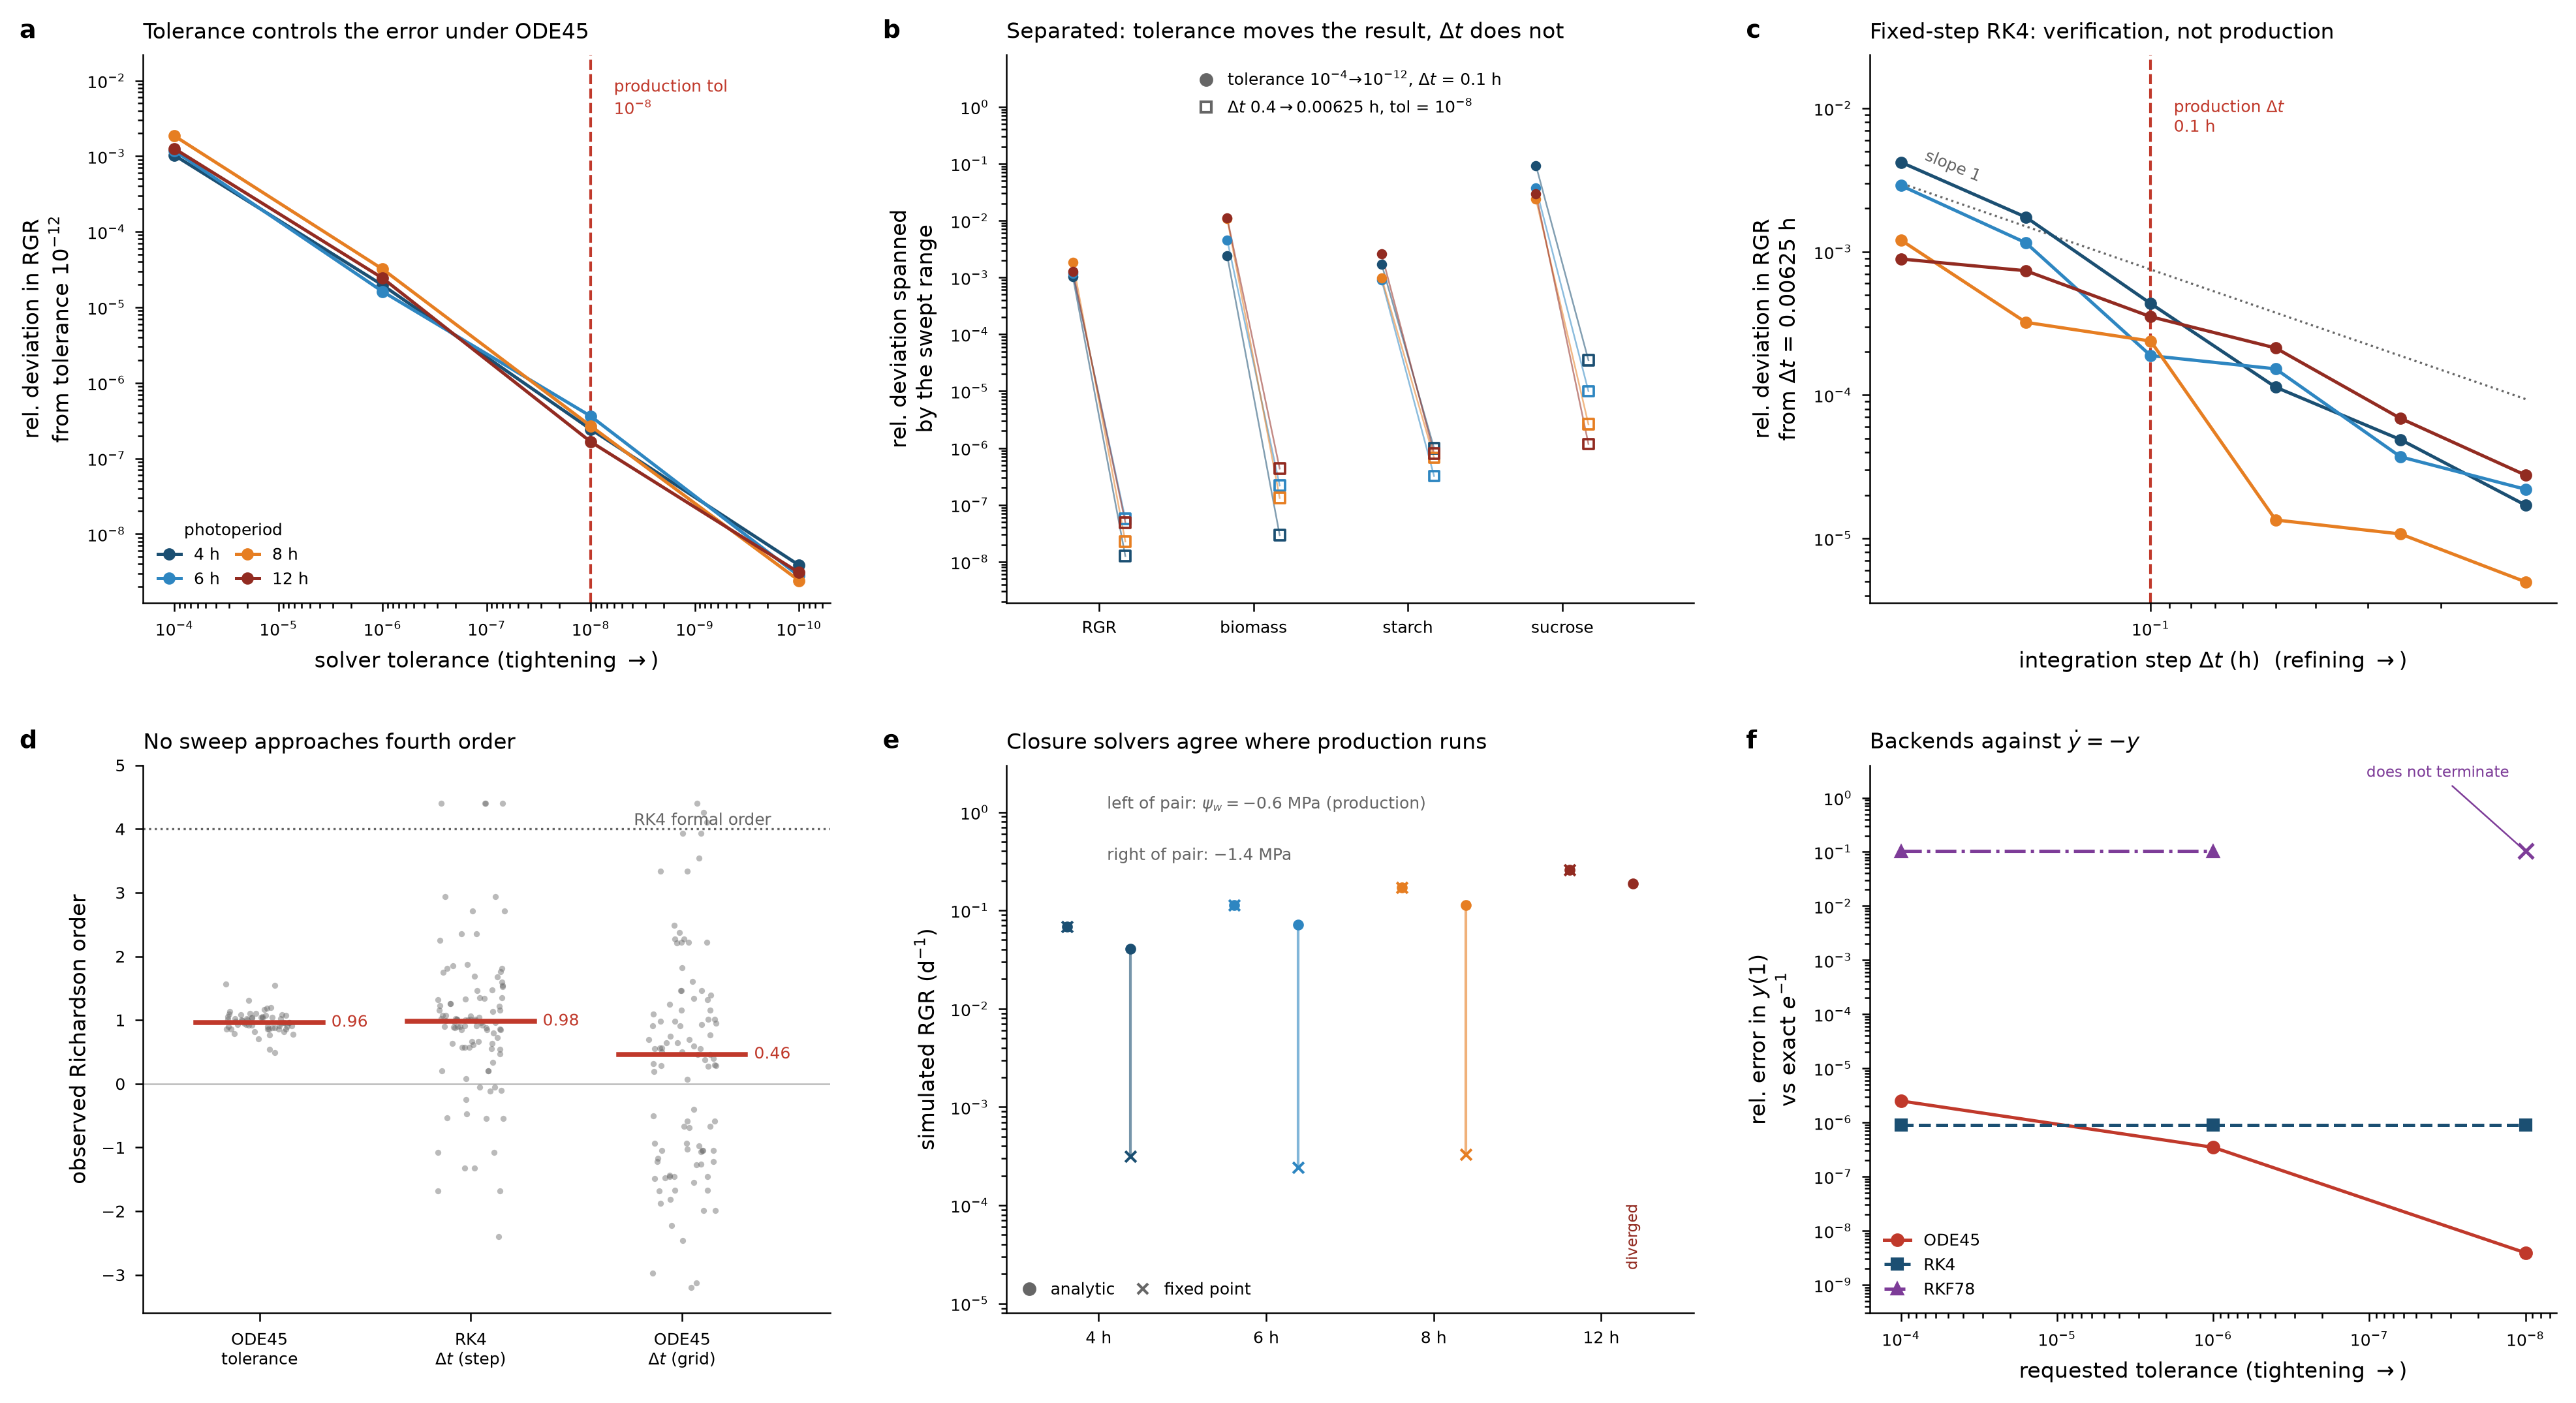
\includegraphics[width=\textwidth]{convergence_study.png}
\caption{Convergence of the numerical procedure. (a) Relative deviation of RGR
from the tightest tolerance ($10^{-12}$) against solver tolerance, per
photoperiod, at the production reporting interval $\Delta t = 0.1$~h; the
production tolerance $10^{-8}$ is marked. Under the adaptive \texttt{ODE45}
backend used for all reported runs, the tolerance is the quantity that controls
the discretisation error, so this is the production-relevant convergence test.
(b) The two error sources separated: for each metric, the relative deviation
spanned by the tolerance sweep at fixed $\Delta t$ (filled) against that spanned
by the $\Delta t$ sweep at fixed tolerance (open). Because \texttt{dt\_hours} is
the initial step and the output interval rather than the integration step, the
$\Delta t$ span is an output-grid effect and is three to five orders of
magnitude smaller. (c) Fixed-step \texttt{RK4} step refinement, shown as
verification of the integrator and not as the production configuration; here
$\Delta t$ is the integration step and the error falls monotonically with a
slope near one. (d) Observed Richardson exponent by sweep, with medians marked;
the formal fourth order of the Runge--Kutta scheme is shown for reference and is
approached by none of the three, since the forcing and several constitutive laws
are only piecewise smooth in time. The \texttt{ODE45} $\Delta t$ exponent is
output-grid noise, not an order of convergence. (e) Analytic versus fixed-point
closure at two leaf water potentials: indistinguishable at the calibrated
$\psi_w = -0.6$~MPa with zero non-convergent solves, and a near-total collapse
of simulated growth at $-1.4$~MPa, where $96$--$97\%$ of solves reach the
iteration cap; the 12~h fixed-point run there diverges outright and is marked as
such rather than plotted as a small value. (f) Verification of the three library
integrators against the exact solution of $\dot y = -y$: \texttt{ODE45}
converges with tolerance, fixed-step \texttt{RK4} is tolerance-independent as
expected, and \texttt{RKF78} returns a $10\%$ error at both tolerances at which
it terminates and does not terminate at $10^{-8}$. All panels: 35-day
integration, four photoperiods, the default configuration
\protect\path{config/default.config}.}
\label{fig:convergence_study}
\end{figure}

% ============================================================
\section{Model Evaluation Protocol}
\label{sec:evaluation_protocol}

The model was evaluated under controlled photoperiod scenarios using
\textit{Arabidopsis thaliana} targets drawn from published metabolite and
growth measurements, principally the photoperiod series of
\citet{Sulpice2014}, which supplies the relative-growth-rate targets, together
with the diel carbohydrate time courses of \citet{Annunziata2017} and the
photoperiod trends of \citet{Mengin2017}. The evaluation was
designed to test three complementary aspects of the proposed simulation
workflow: the ability to reproduce photoperiod-dependent relative growth rate
(RGR), the ability to generate physiologically plausible day-night
carbohydrate dynamics, and the robustness of the coupled model with respect to
parameter variation.

\subsection{Photoperiod scenarios}

Four photoperiod treatments were considered: 4 h, 6 h, 8 h, and 12 h of light
per 24 h cycle (Table~\ref{tab:scenarios}). These scenarios provide a
controlled way to perturb the balance
between daytime carbon assimilation and nighttime reserve mobilization. Each
simulation was run for 30 days, and the reported carbohydrate dynamics were
analysed after the transient response had reached a repeating diel pattern.

\begin{table}[!htbp]
\centering
\small
\caption{Photoperiod validation scenarios. All non-photoperiod forcing is
identical across scenarios and taken from \texttt{config/default.config};
only the light schedule changes. PAR follows a half-sinusoid
$\mathrm{PAR}(t)=\mathrm{PAR}_{\max}\sin(\pi t/P)$ over the light phase, so
with a photoperiod-independent $\mathrm{PAR}_{\max}$ the mean daytime
irradiance is the same in every scenario
($2\,\mathrm{PAR}_{\max}/\pi = 764\ \mu\mathrm{mol\,m^{-2}\,s^{-1}}$) and the
daily light integral (DLI) scales in proportion to day length. Photoperiod
and photon dose are therefore deliberately confounded in this design; see the
discussion of Table~\ref{tab:dli} below.}
\label{tab:scenarios}
\begin{tabular}{lllrrl}
\toprule
\textbf{Sc.} & \textbf{Photoperiod} & \textbf{Dur.} &
\textbf{PAR$_{\max}$} & \textbf{DLI} & \textbf{Evaluation target} \\
             &                      &               &
\multicolumn{1}{c}{\footnotesize $\mu$mol m$^{-2}$ s$^{-1}$} &
\multicolumn{1}{c}{\footnotesize mol m$^{-2}$ d$^{-1}$} & \\
\midrule
S1 & 4 h light / 20 h dark  & 30 d & 1200 & 11.00 & RGR, day--night carbohydrates \\
S2 & 6 h light / 18 h dark  & 30 d & 1200 & 16.50 & RGR, day--night carbohydrates \\
S3 & 8 h light / 16 h dark  & 30 d & 1200 & 22.00 & RGR, day--night carbohydrates \\
S4 & 12 h light / 12 h dark & 30 d & 1200 & 33.00 & RGR, day--night carbohydrates \\
\midrule
\multicolumn{6}{@{}l}{\footnotesize Shared forcing: $T=25\ ^\circ$C,
RH $=60\%$, $C_a=400\ \mu$mol mol$^{-1}$,
$\psi_w=-0.6$ MPa, SLA $=0.025$ m$^2$ gFW$^{-1}$;} \\
\multicolumn{6}{@{}l}{\footnotesize initial state
$B_l=B_r=0.02$ gFW, sunrise at $t=0$ h.} \\
\bottomrule
\end{tabular}
\end{table}

Two properties of this design must be stated explicitly, because both
affect how the photoperiod results should be read.

First, photoperiod and daily photon dose are confounded. Holding
$\mathrm{PAR}_{\max}$ fixed while lengthening the day increases DLI in
proportion to day length, so the 12~h scenario receives three times the
photon dose of the 4~h scenario (Table~\ref{tab:scenarios}). A change in
simulated RGR across scenarios therefore reflects the joint effect of day
length and integrated irradiance, not day length alone. This matches the
design of the reference experiments, in which irradiance was also held
constant while photoperiod was varied, so the comparison to the observed
RGR series is consistent; but it means that neither the observations nor
the simulation isolate a pure photoperiod effect, and the ablation and
sensitivity results in Sections~\ref{sec:results} onward are interpreted
accordingly. \citet{Mengin2017} separated the two factors experimentally at
6 and 12~h and found starch allocation to be sensitive to photoperiod but
largely insensitive to irradiance, which supports attributing most of the
observed response to day length; reproducing that factorial design in
simulation is left to future work.

Second, the absolute irradiance level is higher than in the reference
experiments. The reference photoperiod series was grown under approximately
rectangular chamber lighting of order
$150\ \mu\mathrm{mol\,m^{-2}\,s^{-1}}$, giving DLI values of roughly
$2.2$--$6.5\ \mathrm{mol\,m^{-2}\,d^{-1}}$ across 4--12~h, whereas the
half-sinusoidal schedule used here delivers
$11.0$--$33.0\ \mathrm{mol\,m^{-2}\,d^{-1}}$ --- a factor of $5.1$ higher at
matched day length (Table~\ref{tab:dli}). The half-sinusoid was chosen to give
continuous, differentiable forcing through dawn and dusk, which the
adaptive integrator handles without step rejection at a light--dark
discontinuity, and it is the natural profile for the outdoor conditions the
model is ultimately intended for \citep{Annunziata2017}. The consequence is
that the fitted carbon-input coefficient $\kappa'$
(Eq.~\ref{eq:kappa_prime}) absorbs this irradiance mismatch along with the
leaf-to-rosette scaling: a model driven at five times the experimental
photon dose must retain a correspondingly smaller fraction of the
per-area assimilation to reproduce the observed growth. This is a
recognised limitation of the present forcing specification rather than a
physiological result, and it is one reason the per-photoperiod calibration
in Section~\ref{sec:results} cannot be read as parameter estimation.

\begin{table}[!htbp]
\centering
\small
\caption{Daily light integral of the simulated forcing compared with the
approximate DLI of the reference growth-chamber experiments. Simulated
values are the exact integral of the half-sinusoid,
$\mathrm{DLI}=2\,\mathrm{PAR}_{\max}P/\pi$ converted to
mol m$^{-2}$ d$^{-1}$; reference values assume rectangular lighting at
$150\ \mu\mathrm{mol\,m^{-2}\,s^{-1}}$.}
\label{tab:dli}
\begin{tabular}{@{}lrrr@{}}
\toprule
Photoperiod & Simulated DLI & Reference DLI & Ratio \\
            & \multicolumn{1}{c}{\footnotesize mol m$^{-2}$ d$^{-1}$}
            & \multicolumn{1}{c}{\footnotesize mol m$^{-2}$ d$^{-1}$} & \\
\midrule
4 h  & 11.00 & 2.16 & 5.1 \\
6 h  & 16.50 & 3.24 & 5.1 \\
8 h  & 22.00 & 4.32 & 5.1 \\
12 h & 33.00 & 6.48 & 5.1 \\
\bottomrule
\end{tabular}
\end{table}

\subsection{RGR validation metric}

The primary growth-level validation metric was relative growth rate:
\begin{equation}
RGR =
\frac{\ln B(t_2) - \ln B(t_1)}
{t_2 - t_1},
\end{equation}
where $B(t)$ denotes total plant biomass at time $t$. The simulated RGR was
compared against the photoperiod-specific RGR targets reported for
\textit{Arabidopsis thaliana} rosettes by \citet{Sulpice2014}
($RGR_{\mathrm{ref}} = 0.068$, $0.114$, $0.171$ and $0.260~\mathrm{d}^{-1}$
for the 4, 6, 8 and 12~h photoperiods, respectively). These four values are
from \citet{Sulpice2014} and not, as the original submission stated, from
\citet{Annunziata2017}, whose photoperiod series does not report RGR at all
four of these day lengths; the attribution is corrected here and the numerical
targets are unchanged. The
relative error was computed as:
\begin{equation}
E_{\mathrm{rel}} =
100
\frac{\hat{RGR} - RGR_{\mathrm{ref}}}
{RGR_{\mathrm{ref}}},
\end{equation}
where $\hat{RGR}$ is the simulated value and $RGR_{\mathrm{ref}}$ is the
reference value.

The in-sample RGR comparison cannot be interpreted as a validation at all,
and is reported as a calibration diagnostic. The calibration adjusts two
coefficients per photoperiod --- the growth coefficient $\lambda_{sb}$ and
the starch-synthesis rate $\lambda_{sdi}$ --- by nested bisection against
exactly two observations per photoperiod, the published RGR and the published
end-of-day starch content. The fitted model is therefore saturated: eight
parameters, eight observations, zero degrees of freedom, and the residual
that a bisection leaves behind is a convergence tolerance rather than a
prediction error. To separate the two, the protocol adds an out-of-sample
test in which a single photoperiod-independent parameter pair is fitted on
the 8 and 12~h treatments and used to predict the 4 and 6~h treatments; the
split is by photoperiod rather than at random, because interpolation within
the photoperiod range is exactly the ability in question. Both regimes are
reported in Section~\ref{sec:results}. The carbohydrate dynamics, ablation
behaviour and sensitivity structure are used as evidence in their own right,
not as a substitute for the missing degrees of freedom.

\subsection{Carbohydrate validation metrics}
\label{sec:carbohydrate_metrics}

Sucrose and starch dynamics were evaluated against the measured day-night
carbohydrate profiles of \citet{Annunziata2017}, which provide the primary
reference for the shape and timing of the diel cycle at the 12~h photoperiod,
supported by \citet{Mengin2017} at 6 and 12~h and by the photoperiod trends of
\citet{Sulpice2014}. No single published source supplies matched diel time
courses at all four photoperiods studied here, so the comparison is against the
12~h reference curves for shape and against the photoperiod trend for the
remaining day lengths. Because the available reference data were
used primarily to evaluate the timing and shape of day-night dynamics, the
comparison was performed using scale-adjusted error metrics. For each
photoperiod, sucrose and starch were compared at matching reference time
points.

Concretely, a single multiplicative scale $\alpha$ is fitted by least squares
to each simulated trace before the error is evaluated, so that the metrics
score the shape and timing of the diel cycle rather than the absolute level:

\begin{equation}
\alpha =
\frac{\sum_{i=1}^{n} \hat{y}_i \, y_i}
     {\sum_{i=1}^{n} \hat{y}_i^{\,2}},
\qquad
r_i = \alpha \hat{y}_i - y_i .
\end{equation}

The following error metrics were then computed on the scaled residual $r_i$:
\begin{equation}
MAE =
\frac{1}{n}
\sum_{i=1}^{n}
\left|
r_i
\right|,
\end{equation}

\begin{equation}
RMSE =
\sqrt{
\frac{1}{n}
\sum_{i=1}^{n}
r_i^2
},
\end{equation}

\begin{equation}
nRMSE =
\frac{RMSE}
{\left| \bar{y} \right|},
\qquad
\bar{y} = \frac{1}{n}\sum_{i=1}^{n} y_i .
\end{equation}

Here, $y_i$ denotes the reference value, $\hat{y}_i$ denotes the simulated
value, $n$ is the number of available reference points, and $\bar{y}$ is the
mean reference level, which normalises the RMSE. $MAE$ retains the units of
the reference data ($\mu$mol\,gFW$^{-1}$) and is reported for the same fitted
$\alpha$, so the normalised and absolute errors describe one and the same fit.
The three quantities are computed by \protect\path{fit_scaled_nrmse} in
\protect\path{tools/validation_runner.c}. The predefined
acceptance thresholds were $nRMSE < 0.50$ for sucrose and $nRMSE < 0.25$ for
starch.

\subsection{Ablation protocol}

An ablation study was performed to isolate the contribution of the
photosynthesis and gas-exchange components. Three model variants were compared
using the same downstream growth framework (Table~\ref{tab:ablation_variants}):

\begin{table}[!htbp]
\centering
\caption{Ablation variants used to test the contribution of the gas-exchange layer.}
\label{tab:ablation_variants}
\begin{tabular}{ll}
\toprule
\textbf{Variant} & \textbf{Description} \\
\midrule
M0 - Basic &
Tedone-style baseline with prescribed carbon input. \\

M1 - Farquhar &
Baseline model with Farquhar C$_3$ biochemical photosynthesis
and fixed conductance. \\

M2 - Farquhar-Jarvis &
Farquhar photosynthesis coupled with Jarvis stomatal regulation. \\
\bottomrule
\end{tabular}
\end{table}

The three variants differ only in how the carbon input $\Phi_c$ is produced. Every
downstream equation --- the carbohydrate, nutrient and biomass dynamics of
Sections~\ref{sec:carbohydrates} onward --- is byte-identical across variants,
and so is every parameter that appears in them. Explicitly:

\begin{itemize}
\item \textbf{M0 (Basic)} prescribes the carbon input as a saturating
      multiplicative form with no gas-exchange representation:
      \begin{equation}
      \Phi_{c,M0} = L(t)\;\Lambda(a)\;\Phi_{c,\max}\;
                \min\!\left(\sigma_N,\ \sigma_P\right),
      \label{eq:m0}
      \end{equation}
      where $L(t)\in\{0,1\}$ is the light switch, $\Phi_{c,\max}$ a prescribed
      maximum rate ($12.7\ \mu\mathrm{mol\,gFW^{-1}\,h^{-1}}$),
      $\sigma_N,\sigma_P$ the nutrient-saturation factors, and $\Lambda(a)$
      the starch feedback on the photosynthetic rate,
      \begin{equation}
      \Lambda(a) = \lambda_c
        + \left(1-\lambda_c\right)\frac{a_{\max}-a}{a_{\max}},
      \qquad a_{\max} = D_{a,\max}\left(24 - P\right),
      \label{eq:starch_feedback}
      \end{equation}
      with $\lambda_c$ the photoperiod-specific feedback coefficient of
      Table~\ref{tab:symbols} and $D_{a,\max}$ the maximum starch
      degradation rate. This term is active in M0 only; in M1 and M2 the
      carbon input is set by the gas-exchange solution and $\Lambda$ does
      not enter. Neither $C_i$,
      $g_s$, PAR intensity, temperature, humidity nor $C_a$ appears: the
      carbon input responds to day length and internal state only, which is
      the formulation the coupled model is intended to replace.

\item \textbf{M1 (Farquhar)} computes $A_n$ from the full
      Farquhar--von Caemmerer--Berry biochemistry, but does not solve the
      supply--demand closure. Conductance is held at the fixed value
      $g_s = 0.1\ \mathrm{mol\,m^{-2}\,s^{-1}}$ from
      \texttt{config/default.config}, so $C_i$ still satisfies the same
      diffusion constraint
      $C_i = C_a - A_n/(g_s/1.6)$ and is obtained by the same closed-form
      solution, but with a $g_s$ that does not respond to the environment:
      \begin{equation}
      \Phi_{c,M1} = \kappa'\,3600\,\mathrm{SLA}\,
                A_n\!\left(C_i;\ g_s = \bar{g}_s\right),
      \qquad \bar{g}_s = 0.1 .
      \label{eq:m1}
      \end{equation}
      M1 therefore isolates the effect of biochemical demand alone.

\item \textbf{M2 (Farquhar--Jarvis)} is the full model:
      $g_s$ is computed by the Jarvis multiplicative response
      (Eq.~\eqref{eq:jarvis_general}) from PAR, VPD, temperature, $C_a$ and
      $\psi_w$, and the closure is solved for $C_i$ and $A_n$
      simultaneously, giving Eq.~\eqref{eq:conversion}.
\end{itemize}

The design point is that M0 $\to$ M1 adds biochemical demand, and
M1 $\to$ M2 adds mechanistic stomatal supply. Because the fitted coefficients
$\lambda_{sb}$ and $\lambda_{sdi}$ are held at the values obtained for M2 in
every variant (see below), the comparison is not confounded by per-variant
recalibration.

The purpose of this experiment was not only to compare reported RGR error, but
also to test whether the proposed gas-exchange layer provides an
environment-responsive carbon input that can be propagated into downstream
carbohydrate and biomass dynamics.

\subsection{Sensitivity analysis protocol}
\label{sec:sensitivity_protocol}

Sensitivity analysis was performed using three complementary approaches. First,
one-at-a-time parameter sweeps were used to inspect the direction, saturation,
and threshold behaviour of the RGR response. Second, Morris screening was used
to identify parameters with large elementary effects and to distinguish
approximately linear effects from nonlinear or interaction-driven effects.
Third, Sobol' total-order indices were used to estimate the global contribution
of each parameter to RGR variability, including interaction effects. The
parameters examined were organised into functional groups spanning nutrient
uptake, gas exchange, water and temperature status, respiration, and initial
conditions (Table~\ref{tab:sensitivity_parameter_groups}).

\begin{table}[!htbp]
\centering
\caption{Parameter groups used in the sensitivity analysis.}
\label{tab:sensitivity_parameter_groups}
\begin{tabular}{lll}
\toprule
\textbf{Group} & \textbf{Parameters} & \textbf{Interpretation} \\
\midrule
Nutrient uptake capacity & $I_{N,\max}$, $I_{P,\max}$ & Potential N and P acquisition capacity \\
Soil nutrient content & $N_s$, $P_s$ & External nutrient availability \\
Gas exchange and light & $V_{cmax}$, $J_{\max}$, $C_a$, RH, PAR$_{\max}$ & Photosynthetic and stomatal response \\
Water and temperature & $\psi_w$, $T$ & Abiotic limitation of gas exchange and growth \\
Respiration and growth & $r_m$, $\lambda_{sb}$ & Carbon loss and growth-rate scaling \\
Initial conditions & $s_0$, $B_0$ & Initial carbohydrate and biomass state \\
Vacuolar exchange & $k_{in}$ & Sucrose exchange with vacuolar compartment \\
\bottomrule
\end{tabular}
\end{table}

The sensitivity analysis focused on parameters related to nutrient uptake,
water status, gas exchange, light response, respiration, and initial
carbohydrate or biomass states. The main output analysed in this section was
RGR. The admissible range, sampling scale (linear or logarithmic), functional
role and literature basis of each of the $d=16$ sampled parameters are given
individually in Appendix~\ref{app:sensitivity_params}, which reproduces the
machine-readable parameter specification used by the sensitivity driver.
Table~\ref{tab:evaluation_outputs} summarises all evaluation outputs and
the analysis stage in which each is used.

\subsubsection{Sampling design and verification of the estimators}
\label{sec:sa_design}

Because the sensitivity indices are themselves the output of a Monte Carlo
estimator, the sampling design and the estimator were specified and tested
before being applied to the model. Total-order Sobol' indices $S_T$ and
first-order indices $S_1$ were computed with the estimators of
\citet{Sobol2001} in the form recommended by \citet{Saltelli2010}, which
requires two \emph{independent} base sample matrices $\mathbf{A}$ and
$\mathbf{B}$ of size $n \times d$ and evaluates the model on the $d$ hybrid
matrices $\mathbf{A}_{\mathbf{B}}^{(i)}$ obtained by substituting column $i$
of $\mathbf{A}$ with column $i$ of $\mathbf{B}$, for a total of $n(d+2)$
model runs. The independence requirement is not a formality: the estimator
attributes variance to parameter $i$ through the change produced by that
single-column substitution, so any correlation between the corresponding
columns of $\mathbf{A}$ and $\mathbf{B}$ biases the index towards zero.
Splitting one low-discrepancy sequence of length $2n$ into a first and a
second half does \emph{not} produce independent matrices, and
Section~\ref{sec:results} reports what that construction does to the
estimates.

The base matrices are therefore constructed by one of two designs, selected
at run time according to the dimension of the problem. When $2d$ does not
exceed the maximum dimension supported by the low-discrepancy sampler, a
single Sobol' sequence in $2d$ dimensions is drawn and split by
\emph{column}, the construction specified by \citet{Saltelli2010}. When it
does --- as here, where $d=16$ and the sampler is limited to 16 dimensions
--- two independent Latin-hypercube samples are drawn instead, stratified
per dimension and independent by construction \citep{McKay1979}. The design
actually used is written to a \texttt{base\_design} column in every output
file, so that no reported index is ambiguous about its own provenance.

The estimator implementation was verified against the Ishigami function
\citep{Ishigami1990},
\begin{equation}
f(x_1,x_2,x_3) = \sin x_1 + 7\sin^2 x_2 + 0.1\,x_3^4 \sin x_1 ,
\qquad x_i \sim \mathcal{U}(-\pi,\pi),
\label{eq:ishigami}
\end{equation}
whose first- and total-order indices are known in closed form, so that the
estimator can be tested rather than assumed correct. Convergence was
assessed as the mean absolute error against the analytic indices over eight
seeds, for $n$ from $256$ to $16384$.

Uncertainty in the model indices is reported at two levels, because the two
levels answer different questions. Bootstrap confidence intervals
($10^3$ resamples of the model evaluations) quantify sampling noise
\emph{given} a design and are blind to error contributed by the design
itself; a replicate-design spread, obtained by repeating the whole analysis
with ten independently generated base samples, quantifies the latter. Both
are reported for every index.

Morris screening followed \citet{Morris1991} with the elementary-effect
measures $\mu^\ast$ and $\sigma$ of \citet{Campolongo2007}, using $r$
trajectories with a $p$-level grid and a fixed step $\Delta = p/[2(p-1)]$.
Morris trajectory base points are drawn from an independent pseudo-random
generator rather than from the low-discrepancy sampler, as the method
specifies, so the screening results are not affected by the base-sample
construction discussed above.

\begin{table}[!htbp]
\centering
\caption{Evaluation outputs and their role in the analysis.}
\label{tab:evaluation_outputs}
\begin{tabular}{lll}
\toprule
\textbf{Output} & \textbf{Used in} & \textbf{Purpose} \\
\midrule
RGR & Growth validation, ablation, sensitivity & Main growth-level response \\
Sucrose & Carbohydrate validation & Mobile carbon dynamics \\
Starch & Carbohydrate validation & Day-night reserve dynamics \\
$\Phi_c$ & Numerical checks & Photosynthetic carbon input consistency \\
$s_{cyt}$ & Numerical checks & State validity and carbohydrate stability \\
Biomass & RGR computation and state checks & Growth state consistency \\
Sobol' $S_T$ & Global sensitivity & Parameter importance including interactions \\
Morris $\mu^\ast$, $\sigma$ & Screening sensitivity & Effect size and interaction/nonlinearity indication \\
\bottomrule
\end{tabular}
\end{table}

% ============================================================
\section{Results}
\label{sec:results}

The results are presented in five steps. First, the numerical and physiological
validity of the coupled simulations is checked. Second, the calibrated model is
evaluated against photoperiod-dependent RGR targets. Third, the internal
sucrose and starch dynamics are analysed to verify whether the calibrated model
produces plausible day-night carbohydrate behaviour. Fourth, an ablation study is
used to isolate the effect of replacing the simplified carbon-input formulation
with Farquhar and Farquhar-Jarvis gas-exchange models. Finally, global and
local sensitivity analyses are used to identify the dominant sources of RGR
variability.

% ------------------------------
\subsection{Numerical and physiological consistency}

Before analysing the validation and sensitivity results, the simulation output
was checked for numerical and physiological consistency. The coupled model was
required to preserve non-negative sucrose, starch, and biomass states, to
produce no photosynthetic carbon input during the dark phase, and to avoid
nonfinite samples during the 30-day simulation horizon.

\begin{table}[!htbp]
\centering
\caption{Numerical and physiological consistency checks for the
Farquhar-Jarvis model at the repeating day-night cycle. Minima are taken over
all sampled steps of the 30-day run. Generated by
\protect\path{tools/validation_runner.c} into
\protect\path{results/validation/validation_summary.csv}.}
\label{tab:numerical_validation_results}
\begin{tabular}{lrrrrrr}
\toprule
\textbf{PP} &
\textbf{Min. $s_{cyt}$} &
\textbf{Min. starch} &
\textbf{Min. biomass} &
\textbf{Night $\Phi_c$} &
\textbf{Nonfinite} &
\textbf{Pass} \\
\midrule
4 h  & 0.298 & 0.225 & 0.040 & 0.0 & 0 & \checkmark \\
6 h  & 0.423 & 0.225 & 0.040 & 0.0 & 0 & \checkmark \\
8 h  & 0.569 & 0.225 & 0.040 & 0.0 & 0 & \checkmark \\
12 h & 0.908 & 0.225 & 0.040 & 0.0 & 0 & \checkmark \\
\bottomrule
\end{tabular}
\end{table}

All four photoperiod scenarios passed the consistency checks
(Table~\ref{tab:numerical_validation_results}). No negative
sucrose, starch, or biomass values were observed, and no nonfinite values were
detected. The photosynthetic carbon input was zero during the night phase in
all scenarios, confirming that the imposed photoperiod forcing was propagated
consistently into the carbon-input term. These results indicate that the
gas-exchange layer and the downstream carbohydrate, nutrient, and biomass
states remained numerically stable under the evaluated conditions.

% ------------------------------
\subsection{Solver verification and carbon closure}
\label{sec:results_verification}

The consistency checks above are necessary but weak: they test the trajectory
that the calibrated configuration actually produces. The verification tests
of Section~\ref{sec:verification} test the solver over the domain the
sensitivity analysis samples, and they reveal a defect that the calibrated
trajectory does not expose.

\paragraph{The closed form is exact; the fixed-point iteration is not
unconditionally convergent.}
Substituted back into the coupled system, the analytic operating point of
Eq.~\eqref{eq:ci_quadratic} leaves a residual of at most
$6.5\times10^{-14}$ across the PAR sweep, i.e.\ at the level of
double-precision arithmetic. The fixed-point iteration matches it wherever it
converges. It does not always converge. Table~\ref{tab:water_stress} steps
the leaf water potential across the range sampled in the sensitivity
analysis. Down to $\psi_w = -1.0$~MPa not a single daylight solve fails, and
the two solvers agree on daily carbon fixation to $0.1\%$. Between $-1.1$ and
$-1.2$~MPa the behaviour changes abruptly: the non-convergent fraction rises
from $3.50\%$ to $59.75\%$, and the daily fixation reported by the iterative
solver falls $21.5\%$ below the analytic value. By $-1.4$~MPa the iteration
fails in $97.75\%$ of daylight solves and reports $99.9\%$ less carbon fixed
than the exact solution. The transition is sharp, near
$\psi_w \approx -1.15$~MPa, which is why it is invisible in a sweep of the
calibrated configuration: all production runs are performed at
$\psi_w = -0.6$~MPa, where the failure rate is exactly zero.

\begin{table}[!htbp]
\centering
\small
\caption{Fixed-point solver behaviour across the sampled range of leaf water
potential, at fixed remaining forcing. Non-convergence is the fraction of
daylight solves reaching the iteration cap without satisfying
Eq.~\eqref{eq:convergence}. `Carbon deficit' is the shortfall of the daily
integrated fixation reported by the iterative solver relative to the analytic
solution of Eq.~\eqref{eq:ci_quadratic}. All production runs use
$\psi_w=-0.6$~MPa. Abridged from
\protect\path{results/verification/solver_water_stress.csv}.}
\label{tab:water_stress}
\begin{tabular}{@{}rrrrr@{}}
\toprule
$\psi_w$ (MPa) & Solves & Non-conv.\ (\%) & $\int A_n$ analytic (mol~m$^{-2}$) & Carbon deficit (\%) \\
\midrule
$-0.20$ & 2400 & $0.00$  & 0.5671 & 0.11 \\
$-0.60$ & 2400 & $0.00$  & 0.5601 & 0.10 \\
$-1.00$ & 2400 & $0.00$  & 0.5269 & 0.09 \\
$-1.10$ & 2400 & $3.50$  & 0.5047 & 0.10 \\
$-1.20$ & 2400 & $59.75$ & 0.4678 & 21.47 \\
$-1.30$ & 2400 & $87.67$ & 0.4024 & 95.83 \\
$-1.40$ & 2400 & $97.75$ & 0.2755 & 99.92 \\
$-1.50$ & 2400 & $99.25$ & 0.0000 & --- \\
\bottomrule
\end{tabular}
\end{table}

\paragraph{The failure is a period-two orbit, not slow convergence.}
The parity test identifies the mechanism. At a forcing point inside the
failing region, varying the iteration cap over consecutive integers returns
two alternating values and nothing in between: an even cap returns
$A_n = -13.389\ \mu\mathrm{mol\ m^{-2}\ s^{-1}}$ with
$C_i = 862.6\ \mu\mathrm{mol\ mol^{-1}}$, an odd cap returns
$A_n = +23.695$ with $C_i = 0$, and the analytic solution is
$A_n = 7.704$ at every cap. The map has a stable two-cycle, so no increase in
the iteration budget would help; and because the reported value depends on the
parity of the cap, the sign of the flux is determined by an implementation
detail. Neither branch is individually detectable as impossible: the even-cap
pair satisfies the supply relation Eq.~\eqref{eq:diffusion} exactly at the
local conductance ($g_c = 0.029\ \mathrm{mol\ m^{-2}\ s^{-1}}$), and
$C_i > C_a$ is the correct supply solution for the net efflux it reports, so a
bound check on $C_i$ alone would have passed it. What is diagnostic is the pair
taken together --- two mutually inconsistent operating points on the same
forcing, straddling zero assimilation, with the analytic root lying between
them. Cap-parity sensitivity, not a range check on $C_i$, is the test that
would have caught this, and it was not being applied.

\paragraph{Exposure of the sensitivity analysis.}
Over $2\times10^{4}$ parameter vectors drawn from the full ranges of
Appendix~\ref{app:sensitivity_params}, the iterative solver fails to converge
in $15.16\%$ of cases, returns a negative net assimilation under light in
$13.52\%$, and leaves the physically meaningful range with $C_i > 2C_a$ in
$7.64\%$ --- the last a divergence diagnostic in the sense of
Section~\ref{sec:verification}, not a violated model bound. The
discrepancy against the closed form has median zero --- most of the domain is
solved correctly --- but a mean of
$2.43\ \mu\mathrm{mol\ m^{-2}\ s^{-1}}$, a $95$th percentile of $18.72$ and a
maximum of $38.11$, the last comparable in magnitude to the assimilation rate
itself. A sixth of the design points were therefore being evaluated with a
carbon input that was wrong, often with the wrong sign, and the affected
points are not randomly located: they concentrate at low conductance, which is
where the water-status and VPD dimensions act. This is the reason the
sensitivity results were recomputed with the analytic solver, and it is the
reason the local response diagnostics and the validation, diel and ablation
results were not: those are all evaluated at $\psi_w=-0.6$~MPa, inside the
region where the two solvers agree to $0.1\%$.

\paragraph{Corrected Jarvis temperature response.}
The temperature modifier as originally implemented satisfied neither property
its normalisation was intended to guarantee: it returned
$f_T(25^{\circ}\mathrm{C}) = 0.7071$ rather than unity, and its maximum lay
at $32^{\circ}$C rather than at the stated optimum $T_0 = 25^{\circ}$C. Two
independent errors were responsible, one in each normalisation constant of
Eq.~\eqref{eq:jarvis_T}. With both corrected, $f_T(25^{\circ}\mathrm{C}) =
1.000000$, the maximum lies at $25.0^{\circ}$C, and
$f_T(5^{\circ}\mathrm{C}) = f_T(45^{\circ}\mathrm{C}) = 0$ exactly, so the
clipping previously required is not. The correction is calibration-neutral:
because the modifier enters multiplicatively and all calibration runs are
performed at $T = 25^{\circ}$C, setting the explicit $g_{s,\max}$ of
Eq.~\eqref{eq:jarvis_general} equal to the former value $f_T(25)=1/\sqrt{2}$
reproduces the previous conductance at $25^{\circ}$C exactly: across the PAR
range the corrected and previous values agree to within
$3\times10^{-17}\ \mathrm{mol\ m^{-2}\ s^{-1}}$, a relative difference below
$10^{-16}$. No calibrated parameter changes. What changes is
the response away from $25^{\circ}$C, where the corrected conductance is
higher below the optimum and lower above it, by up to a factor of $1.32$ at
$10^{\circ}$C and $0.71$ at $35^{\circ}$C. Results that vary temperature ---
the temperature--humidity and water-potential--temperature surfaces of
Fig.~\ref{fig:parameter_pair_surfaces} and the
\texttt{gas\_exchange.leaf\_temperature} sensitivity dimension --- are
affected and are reported here with the corrected response; results at fixed
$25^{\circ}$C are unchanged bit for bit. Separately, a guard that returned
zero assimilation below $\mathit{PAR} = 20\ \mu\mathrm{mol\ m^{-2}\ s^{-1}}$
was removed. It introduced a genuine discontinuity, since
$f_{\mathit{PAR}}(20) = 0.0374 \neq 0$, and the terminal non-negativity
constraint already yields zero below the light compensation point without a
special case.

\paragraph{Carbon closure.}
Table~\ref{tab:carbon_balance} reports the carbohydrate budget over a 35-day
integration at $\Delta t = 0.1$~h. Assimilated carbon, the starch and sucrose
fluxes, degradation, maintenance respiration, phloem loading, transport
surcharge and vacuolar exchange balance the change in the three
carbohydrate pools to a relative residual between
$1.5\times10^{-15}$ and $1.3\times10^{-14}$ --- machine precision, as it must
be, since the flux accumulators are integrated with the same fixed-step
\texttt{RK4} weights and step as the states in this test
(Section~\ref{sec:verification}). The value of the test is not the
magnitude of the residual but its sensitivity: a mis-signed or double-counted
flux would appear immediately as a residual many orders of magnitude larger,
and during development that is exactly how two bookkeeping errors were found.

The excluded term can now be quantified rather than asserted. The sucrose
drawn from the cytosol to support growth is $\phi_{\text{load}}
E_{\text{night}}$, while the carbon credited to the two biomass pools is
$\lambda_{sb}\,\phi_{\text{load}} E_{\text{night}} B_l$, so the ratio of
credited to withdrawn carbon is exactly $\lambda_{sb} B_l$. With
$\lambda_{sb} = 0.00587\ \mathrm{gFW^{-1}}$ this ratio reaches unity only at
$B_l = 170.4$~gFW, four orders of magnitude above the seedling range
$0.01$--$0.12$~gFW simulated here, over which it spans $5.9\times10^{-5}$ to
$7.0\times10^{-4}$. The biomass equations are therefore an empirical rate law
and not a carbon budget, and $\lambda_{sb}$ is a rate coefficient with units
$\mathrm{gFW^{-1}}$ rather than a carbon-to-fresh-weight yield. We state this
explicitly because the alternative reading --- that the model conserves carbon
from assimilation through to biomass --- is not supported and would be a
straightforward misinterpretation of Table~\ref{tab:carbon_balance}.

\begin{table*}[!htbp]
\centering
\small
\caption{Carbon closure over the carbohydrate subsystem $\{a,s,s_v\}$ for a
35-day integration at $\Delta t=0.1$~h. Fluxes are time-integrated
$\mu\mathrm{mol\ gFW^{-1}}$. The residual is the closure error of the
subsystem budget; the relative residual normalises it by integrated
assimilation. Fresh-weight biomass is outside the budget by construction (see
text). From \protect\path{results/carbon_balance/carbon_balance.csv}.}
\label{tab:carbon_balance}
\begin{tabular}{@{}rrrrrrrr@{}}
\toprule
PP (h) & $\int \Phi_c$ & $\int$ to starch & $\int$ to sucrose & $\int D_a$ & $\int C_{\text{resp}}$ & $\int C_{\text{load}}$ & Rel.\ residual \\
\midrule
4  & 1381.7 & 917.5  & 464.3  & 915.1  & 416.7  & 961.1  & $-3.4\times10^{-15}$ \\
6  & 2069.7 & 1221.5 & 848.2  & 1217.7 & 631.5  & 1429.9 & $-1.5\times10^{-15}$ \\
8  & 2772.3 & 1502.1 & 1270.2 & 1496.9 & 876.8  & 1882.5 & $+4.1\times10^{-15}$ \\
12 & 4146.5 & 2017.5 & 2129.0 & 2010.1 & 1406.2 & 2718.5 & $+1.3\times10^{-14}$ \\
\bottomrule
\end{tabular}
\end{table*}

\begin{figure}[htbp]
\centering
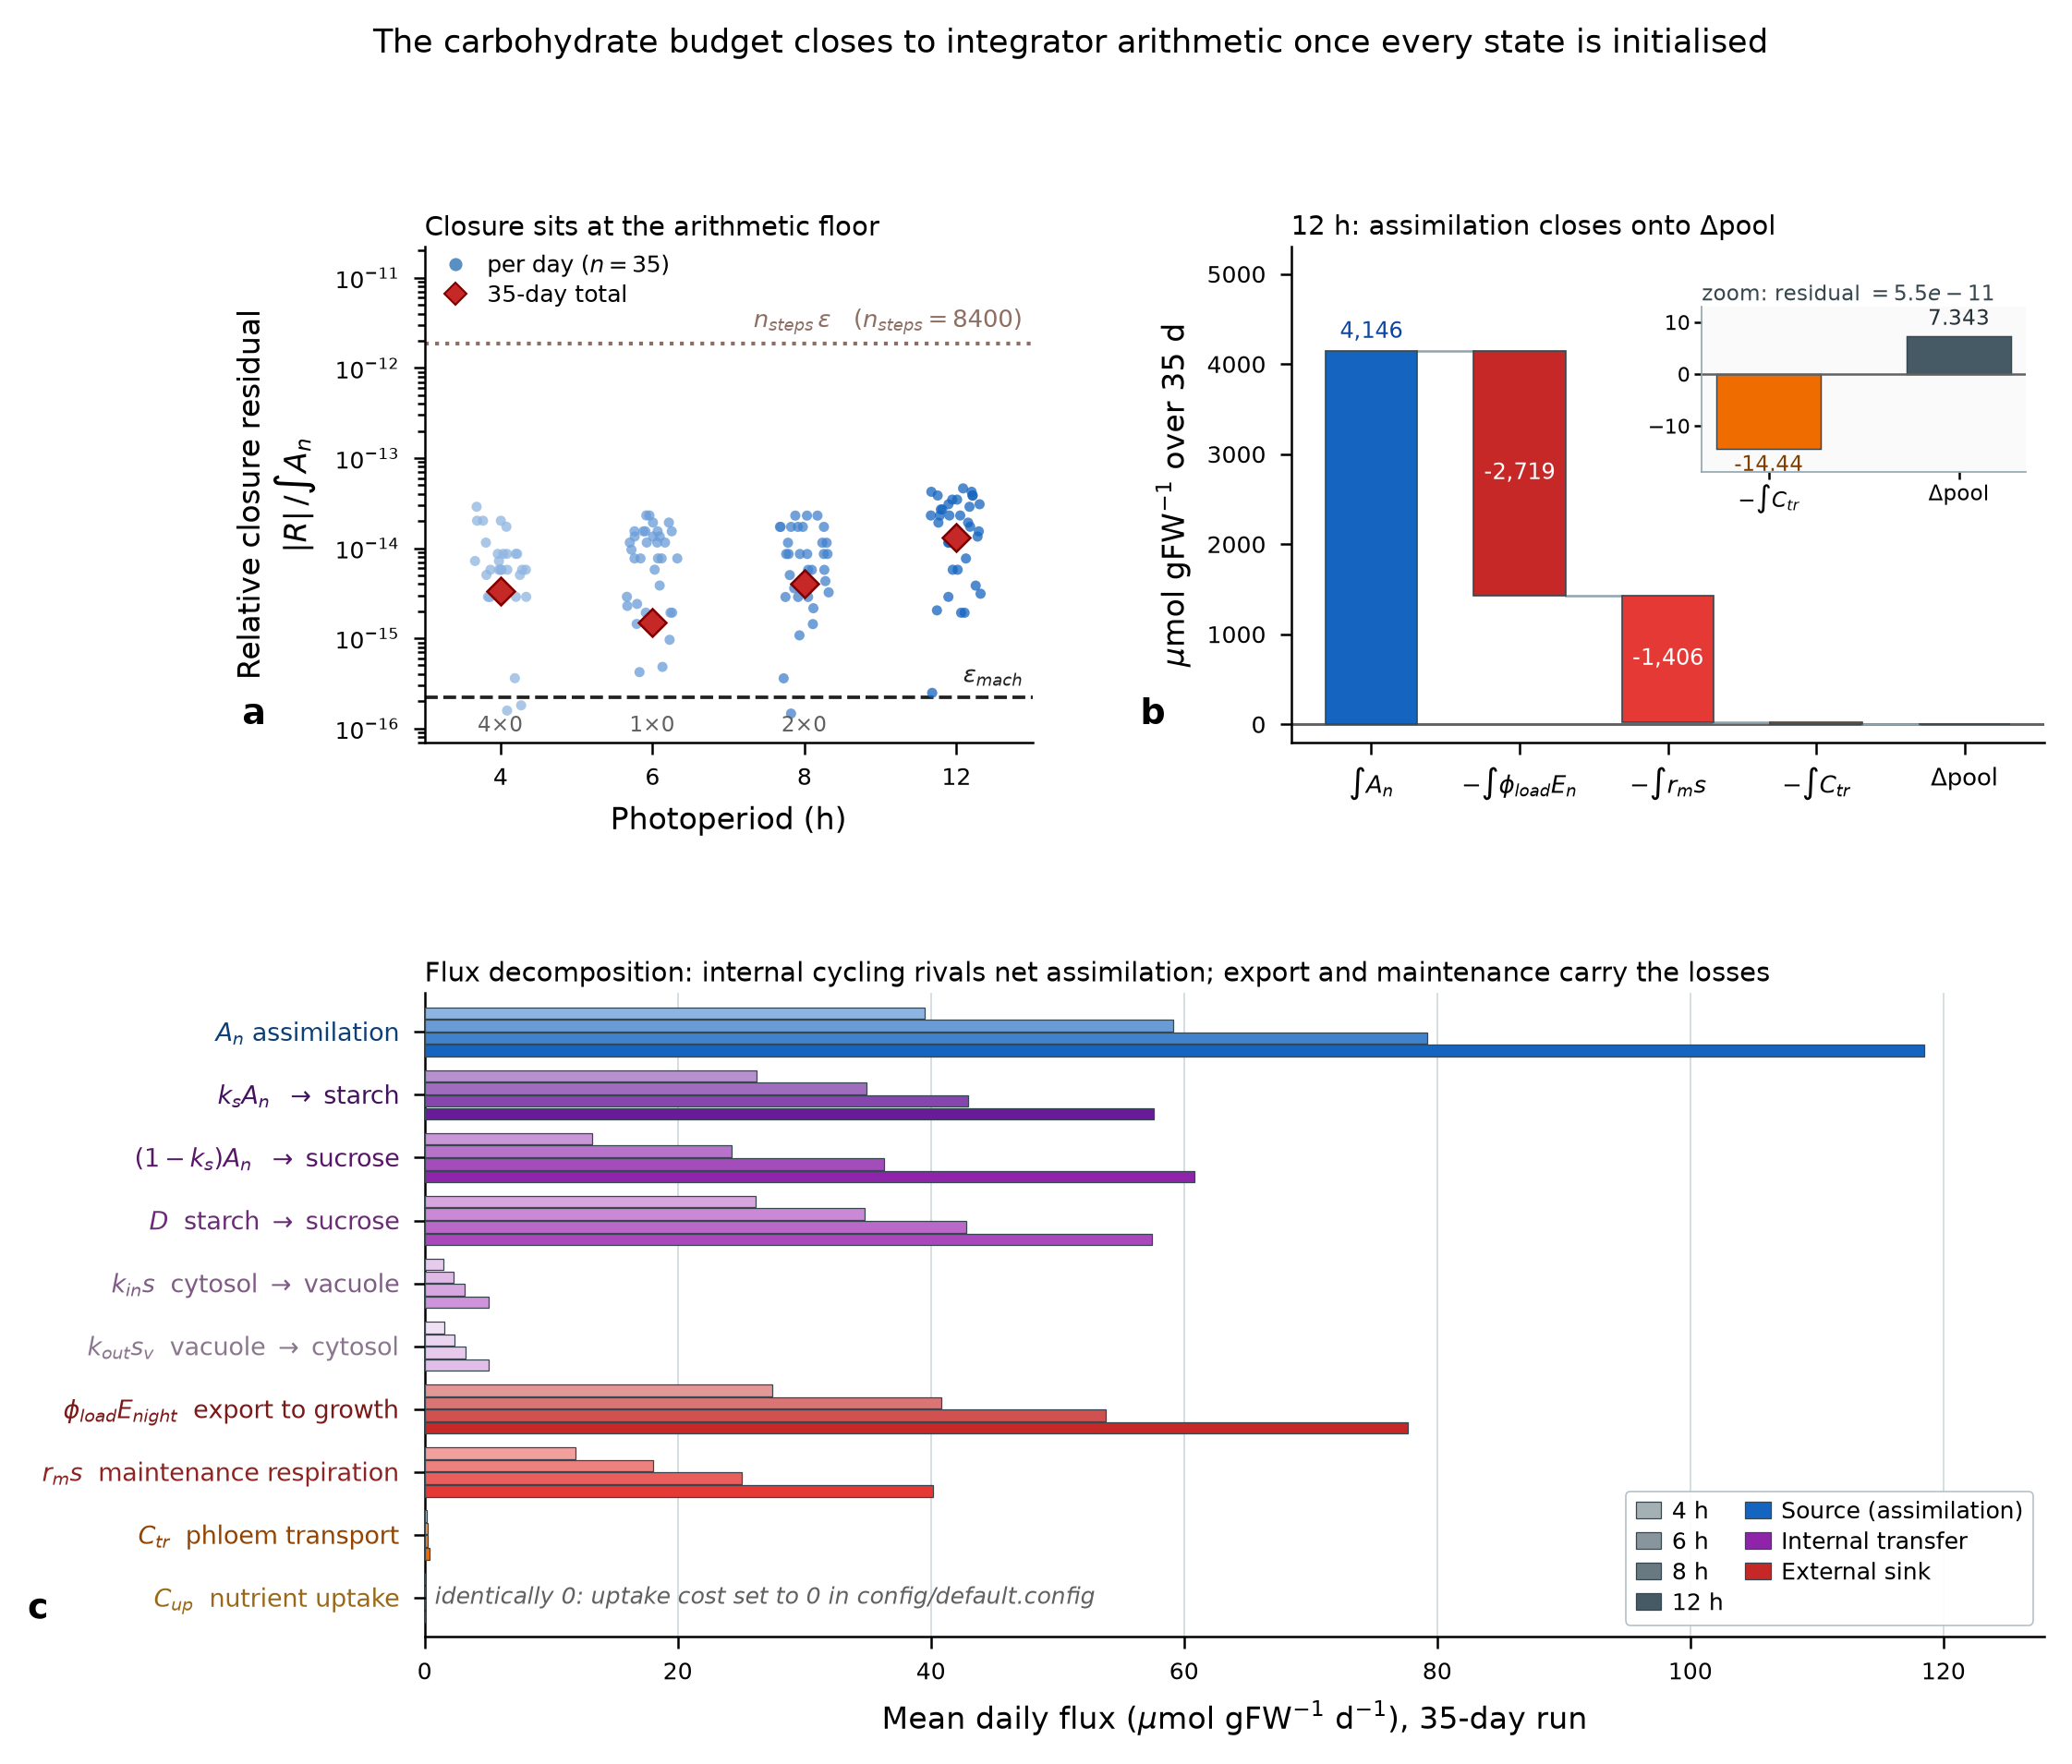
\includegraphics[width=\textwidth]{carbon_balance.png}
\caption{Closure of the carbohydrate budget. (a) Absolute relative closure
residual against photoperiod on a logarithmic axis, per simulated day and for
the 35-day total, with the double-precision machine epsilon and the
accumulated-rounding bound $n_{\text{steps}}\varepsilon$ shown for scale. The
residual sits at the arithmetic floor at every photoperiod, so the closure is
limited by floating-point representation rather than by any modelling
approximation --- the budget is an identity of the discretisation, not an
approximate balance. (b) The 12~h budget as a waterfall: integrated assimilation
against export to growth, maintenance respiration and phloem transport, closing
onto the change in pool size, with the residual shown magnified in the inset.
(c) Decomposition of the mean daily fluxes at all four photoperiods into
assimilation, the two partitioning channels, starch remobilisation, the vacuolar
exchange pair, export to growth, maintenance respiration and transport; nutrient
uptake cost is identically zero because it is set to zero in the production
configuration. Internal cycling is of the same order as net assimilation. In
panels (a) and (c) the annotations \texttt{4$\times$0}, \texttt{1$\times$0} and
\texttt{2$\times$0} record how many of the per-day residuals at that photoperiod
were exactly zero in double precision (4 of the 35 days at 4~h, 1 at 6~h, 2 at
8~h); such days are omitted from the logarithmic axis rather than plotted. This
test integrates the flux accumulators on the augmented system with the same
fixed-step \texttt{RK4} weights and step as the eleven state equations
(Section~\ref{sec:verification}), which is why the residual
reaches machine precision instead of the $10^{-6}$--$10^{-8}$ typical of a
budget reconstructed post hoc from sampled trajectories.}
\label{fig:carbon_balance}
\end{figure}

% ------------------------------
\subsection{Photoperiod-dependent RGR validation}

The calibrated Farquhar-Jarvis model with the vacuolar sucrose compartment
reproduced the RGR targets of \citet{Sulpice2014} across all four photoperiod
scenarios (Table~\ref{tab:rgr_validation_results}, Fig.~\ref{fig:rgr_validation}).
The mean absolute error was $2.41 \times 10^{-4}$, the RMSE was
$2.68 \times 10^{-4}$, and the mean absolute percentage error was $0.24\%$.

\begin{table}[!htbp]
\centering
\caption{RGR validation under photoperiod treatments. The Farquhar-Jarvis model
with vacuolar sucrose compartment was calibrated per photoperiod.}
\label{tab:rgr_validation_results}
\begin{tabular}{lrrrr}
\toprule
\textbf{Photoperiod} &
\textbf{Literature RGR} &
\textbf{Simulated RGR} &
\textbf{Abs. error} &
\textbf{Rel. error (\%)} \\
\midrule
4 h  & 0.0680 & 0.068435 & 0.000435 & 0.640 \\
6 h  & 0.1135 & 0.113679 & 0.000179 & 0.158 \\
8 h  & 0.1708 & 0.170925 & 0.000125 & 0.073 \\
12 h & 0.2600 & 0.260224 & 0.000224 & 0.086 \\
\bottomrule
\end{tabular}
\end{table}

\begin{figure}[htbp]
\centering
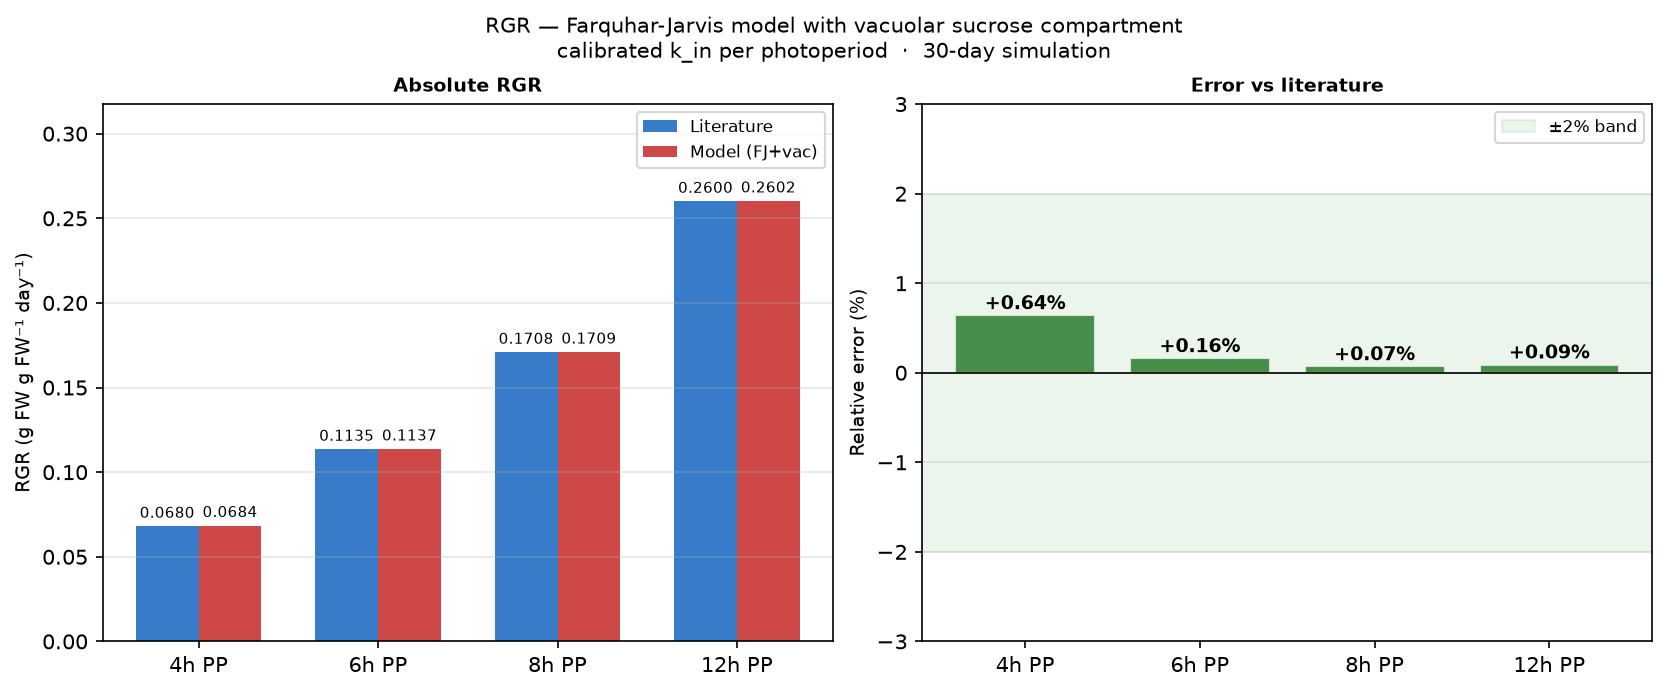
\includegraphics[width=\textwidth]{fj_rgr.png}
\caption{RGR validation of the Farquhar-Jarvis model with vacuolar sucrose
compartment under four photoperiod treatments. The left panel compares absolute
RGR values against the literature targets of \citet{Sulpice2014}, while the
right panel shows the relative
error with respect to the $\pm 2\%$ acceptance band. The model overshoots at
every photoperiod, by at most $0.64\%$; these are convergence residuals of the
per-photoperiod calibration and not predictive errors, as the text below the
figure sets out.}
\label{fig:rgr_validation}
\end{figure}

These residuals must not be read as predictive errors, and the earlier
description of them as ``calibration-consistent validation'' understated the
problem. The calibration procedure adjusts two parameters per photoperiod:
the growth coefficient $\lambda_{sb}$ is bisected until the simulated RGR
equals the published RGR, inside an outer bisection that adjusts the
starch-synthesis rate $\lambda_{sdi}$ until the simulated end-of-day starch
matches the published value. With four photoperiods this is eight fitted
parameters against eight observations: the model is saturated and has zero
degrees of freedom. The numbers in the fourth and fifth columns of
Table~\ref{tab:rgr_validation_results} are therefore convergence residuals
of the bisection, and re-running the calibration to tighter tolerance drives
the RGR error to $0.0000\%$ in every photoperiod. A mean absolute percentage
error of $0.24\%$ measures how well a root-finder converged, not how well the
model predicts. Note also that the parameter identified in the original
submission as the calibrated one --- the vacuolar influx $k_{in}$ --- is not
what the calibration routine adjusts; $\lambda_{sb}$ and $\lambda_{sdi}$ are.

To obtain a figure that does measure prediction, the photoperiod response was
cross-validated out of sample. The design imposes a
photoperiod-\emph{independent} parameterisation, fits it to a subset of
photoperiods, freezes it, and predicts the held-out ones. Two hypotheses were
tested: a \emph{constant} pair $(\lambda_{sb}, \lambda_{sdi})$ shared by all
photoperiods (2 parameters), and a \emph{linear} law
$\lambda_{sb} = c_0 + c_1 P$ with a shared $\lambda_{sdi}$ (3 parameters).
Each was fitted by Nelder--Mead on seven training/test splits --- the three
two-versus-two partitions and the four leave-one-photoperiod-out cases ---
giving 14 cross-validated fits, plus the four saturated per-photoperiod
reference fits: 18 fits in total. Table~\ref{tab:crossval} reports all of
them. Each regime therefore yields ten held-out predictions (two from each
two-versus-two split, one from each leave-one-out split). All ten are
admissible under the constant hypothesis; under the linear hypothesis the
frozen parameters of the \mbox{4, 6~h} training split make one predicted
photoperiod inadmissible, so nine are scored. The aggregate held-out errors
quoted below are means over those ten and nine predictions respectively, not
over the seven splits: an unweighted mean over splits would give $26.32\%$ and
$6.31\%$, and we report the per-prediction figures so that the two-versus-two
splits, which contribute two predictions each, are not under-weighted.

Three conclusions follow, and they point in different directions. First, the
photoperiod dependence of growth in this model is carried substantially by the
calibrated coefficients rather than by the coupled gas-exchange and
carbohydrate dynamics: if it were carried by the dynamics, a single parameter
pair would extrapolate across photoperiod, and it does not --- the constant
hypothesis gives a mean held-out error of $28.49\%$. The model as calibrated
is an interpolator over photoperiod, not a predictor of it. Second, the
deficiency is localised rather than diffuse. Allowing $\lambda_{sb}$ to vary
linearly with photoperiod --- one additional parameter --- reduces the mean
held-out error to $7.27\%$ and the training error to $1.35\%$, so most of the
photoperiod signal the coupled dynamics fail to generate is a smooth,
almost affine trend in a single growth coefficient. That is a considerably
more actionable diagnosis than a global statement of poor prediction, and it
identifies exactly which mechanism a subsequent model version has to supply.
Third, the saturated calibration is not thereby useless --- it is the right
procedure for the question the ablation study asks, which is a comparison
between model variants calibrated identically --- but it cannot support a
claim of predictive accuracy, and no such claim is made here. The held-out
errors, not the in-sample residual, are the figures of merit for
extrapolation across photoperiod, and reducing them is a modelling problem,
not a calibration problem: it would require the photoperiod dependence now
absorbed into $\lambda_{sb}$ and $\lambda_{sdi}$ to be generated by the state
dynamics instead.

\begin{table}[!htbp]
\centering
\small
\caption{Out-of-sample validation of the photoperiod response: all 18 fits.
The \emph{saturated} regime is the manuscript's original procedure --- one
$\lambda_{sb}$ and one $\lambda_{sdi}$ per photoperiod against one RGR and one
end-of-day starch observation per photoperiod (8 parameters, 8 observations,
zero degrees of freedom) --- so its RGR residual is a bisection tolerance and
not an error. The two cross-validated regimes impose a
photoperiod-\emph{independent} law, fit it on the training photoperiods by
Nelder--Mead, freeze it, and predict the held-out ones. Errors are
$|$relative error$|$ in RGR, averaged over the photoperiods in each role.
``n.a.'' marks a predicted photoperiod at which the frozen parameters make the
trajectory inadmissible (the adaptive step collapses; see
Section~\ref{sec:verification_lessons}), recorded rather than scored. The
\textbf{all splits} rows are means over individual held-out predictions --- ten
for the constant regime, nine for the linear regime after the one inadmissible
case --- and not over the seven splits, so that the two-versus-two splits carry
their two predictions each.}
\label{tab:crossval}
\begin{tabular}{@{}llrrrr@{}}
\toprule
Regime & Split & Train & Test & Test & $\lambda_{sdi}$ \\
       &       & MAPE  & MAPE & worst &                \\
\midrule
Saturated (8 par., 8 obs.) & in-sample, all 4 PP  & $0.00$ & --- & --- & per PP \\
\multicolumn{2}{@{}l}{\quad (in-sample end-of-day starch)} & $3.29$ & --- & --- & \\
\midrule
Constant (2 par.) & train 8, 12~h  & $5.62$  & $35.91$ & $46.74$ & $0.0742$ \\
                  & train 4, 6~h   & $8.48$  & $56.19$ & $87.42$ & $0.5708$ \\
                  & train 4, 12~h  & $20.41$ & $8.54$  & $16.34$ & $0.0655$ \\
                  & hold out 4~h   & $10.61$ & $33.27$ & $33.27$ & $0.0897$ \\
                  & hold out 6~h   & $18.36$ & $4.19$  & $4.19$  & $0.0767$ \\
                  & hold out 8~h   & $13.77$ & $16.13$ & $16.13$ & $0.0755$ \\
                  & hold out 12~h  & $11.84$ & $30.02$ & $30.02$ & $0.2890$ \\
\cmidrule(l){2-6}
                  & \textbf{all splits} & $\mathbf{12.93}$ & $\mathbf{28.49}$ & $\mathbf{87.42}$ & \\
\midrule
Linear in $P$ (3 par.) & train 8, 12~h & $0.02$ & $16.70$ & $21.79$ & $0.0727$ \\
                  & train 4, 6~h   & $0.01$ & $4.60$ & $4.60$ & $0.6358$ (1 n.a.) \\
                  & train 4, 12~h  & $0.01$ & $4.52$ & $7.33$ & $0.0596$ \\
                  & hold out 4~h   & $2.88$ & $6.39$ & $6.39$ & $0.0846$ \\
                  & hold out 6~h   & $3.30$ & $0.23$ & $0.23$ & $0.0710$ \\
                  & hold out 8~h   & $0.79$ & $6.96$ & $6.96$ & $0.0694$ \\
                  & hold out 12~h  & $1.09$ & $4.76$ & $4.76$ & $0.3467$ \\
\cmidrule(l){2-6}
                  & \textbf{all splits} & $\mathbf{1.35}$ & $\mathbf{7.27}$ & $\mathbf{21.79}$ & \\
\bottomrule
\end{tabular}
\end{table}

Three things follow from Table~\ref{tab:crossval}. First, the in-sample
residual carries no information about predictive accuracy: it is $0.00\%$ by
construction, while the same model predicting a photoperiod it was not fitted
to is wrong by $7$ to $28\%$ on average and by up to $87\%$ in the worst
split. Second, the comparison between the two cross-validated regimes locates
where the photoperiod dependence lives. A single constant pair cannot
represent it --- $28.49\%$ mean held-out error, and the fit is poor even on its
own training photoperiods ($12.93\%$) --- whereas allowing $\lambda_{sb}$ to
vary linearly with photoperiod reduces held-out error to $7.27\%$ with a
near-exact training fit. The photoperiod response of growth in this model is
therefore carried substantially by a smooth trend in one calibrated
coefficient, not by the coupled dynamics. Third, the splits are not
interchangeable: extrapolation beyond the training range is markedly worse
than interpolation within it. Training on 8 and 12~h and predicting the short
photoperiods gives the largest error of the leave-two-out splits in both
regimes ($35.91\%$ and $16.70\%$), while training on 4 and 12~h and predicting
the interior ($8.54\%$ and $4.52\%$) is the best. The leave-one-out results
show the same ordering, with the interior photoperiods (6 and 8~h) predicted
far more accurately than the endpoints.

One split deserves comment because it exposed a numerical defect rather than a
modelling one. Fitting the linear law on the two shortest photoperiods gives a
poorly determined slope, and the frozen parameters imply $\lambda_{sdi} =
0.636$ at 12~h, beyond the bracket used in calibration; at that value the
adaptive integrator stalls rather than diverging, which is how the step-budget
guard described in Section~\ref{sec:verification_lessons} came to be added. The
affected prediction is reported as non-admissible rather than scored.

The internal carbohydrate trajectories and the ablation and sensitivity
analyses, which do not depend on the RGR fit being predictive, are therefore
the substantive evidence of model behaviour, and are reported next.

% ------------------------------
\subsection{Diel sucrose and starch dynamics}

The model produced stable repeating day-night carbohydrate cycles after the
transient phase. Starch accumulated during the light phase and was depleted
during the dark phase in all photoperiod scenarios
(Fig.~\ref{fig:diel_dynamics}). This behaviour is consistent
with the expected role of transient starch as a daytime carbon reserve and a
nighttime carbon source. Sucrose also showed repeating diel behaviour, although
the agreement with reference sucrose profiles was weaker than for starch at
every photoperiod, and weakest under the short days
(Table~\ref{tab:sugar_starch_validation_results}).

\begin{table}[!htbp]
\centering
\caption{Sugar and starch validation summary. Errors are computed on the
scale-fitted residual of Section~\ref{sec:carbohydrate_metrics}; MAE is in
$\mu$mol\,gFW$^{-1}$ and $\alpha$ is the fitted scale. The scored sucrose
state is the cytosolic pool $s_{cyt}$, which is the pool the reference series
is matched against by the runner; the total (cytosolic plus vacuolar) sucrose
shown in Fig.~\ref{fig:diel_dynamics} is a different quantity and is not
scored here. Each photoperiod was evaluated using 13 reference points from
\protect\path{data/paper/sugars_starch_reference.csv}. Generated by
\protect\path{tools/validation_runner.c} into
\protect\path{results/validation/validation_summary.csv}; the superseded
values of the first submission are retained in
\protect\path{results/validation/validation_summary_2026-07-02.csv}.}
\label{tab:sugar_starch_validation_results}
\begin{tabular}{lrrrrrrr}
\toprule
\textbf{Photoperiod} &
\textbf{Ref. points} &
\textbf{$\alpha_{suc}$} &
\textbf{Sucrose nRMSE} &
\textbf{Sucrose MAE} &
\textbf{$\alpha_{sta}$} &
\textbf{Starch nRMSE} &
\textbf{Starch MAE} \\
\midrule
4 h  & 13 & 3.365 & 0.390 & 0.800 & 1.036 & 0.154 & 1.981 \\
6 h  & 13 & 2.211 & 0.382 & 0.713 & 1.216 & 0.175 & 3.894 \\
8 h  & 13 & 1.971 & 0.315 & 0.683 & 1.052 & 0.192 & 4.453 \\
12 h & 13 & 1.130 & 0.284 & 0.592 & 0.923 & 0.128 & 3.313 \\
\bottomrule
\end{tabular}
\end{table}

\begin{figure}[htbp]
\centering
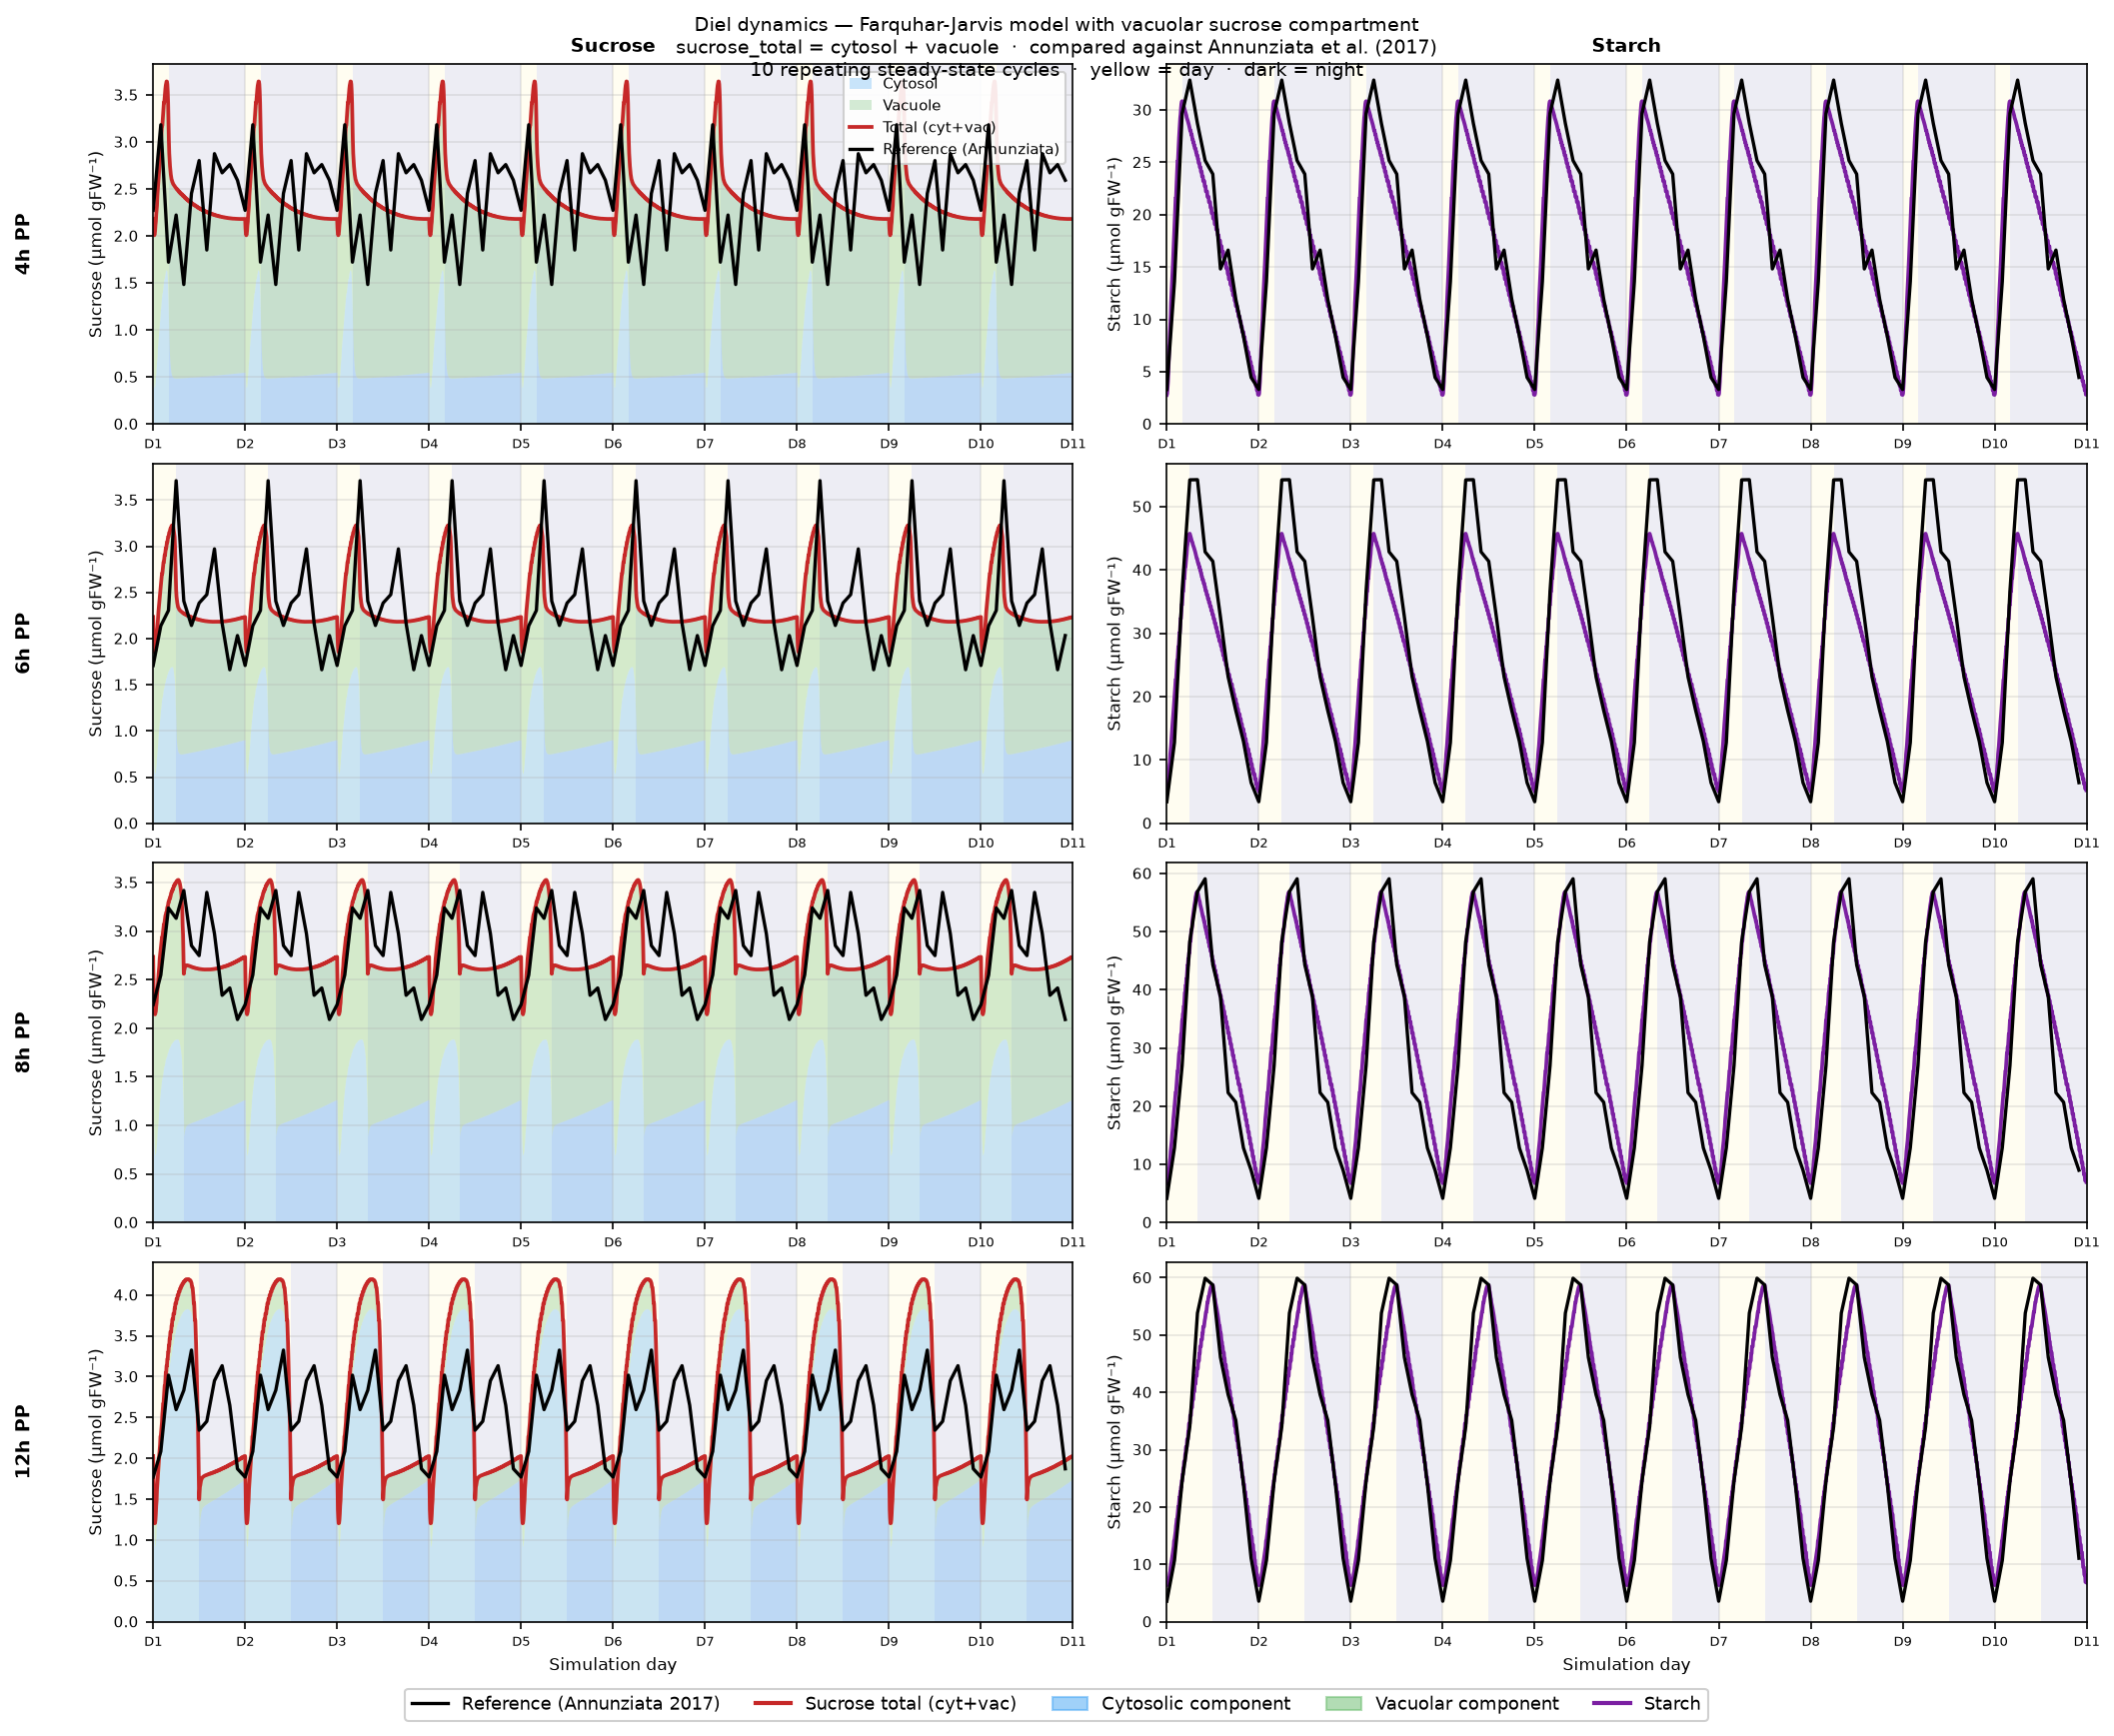
\includegraphics[width=\textwidth]{fj_diel_dynamics.png}
\caption{Diel sucrose and starch dynamics produced by the Farquhar-Jarvis model
with the vacuolar sucrose compartment. Rows are the 4, 6, 8 and 12~h
photoperiods; the left column shows cytosolic, vacuolar and total sucrose and
the right column starch. Black curves are the measured profiles of
\citet{Annunziata2017}. Pale bands mark the light period and grey bands the
dark period, over ten repeating steady-state cycles. Absolute levels carry the
calibration of Section~\ref{sec:results}; the comparison is of shape and
timing (Section~\ref{sec:carbohydrates}).}
\label{fig:diel_dynamics}
\end{figure}

Starch nRMSE remained below the predefined threshold of 0.25 in all scenarios,
with values between 0.128 and 0.192. This indicates that the model captured the
timing and shape of starch accumulation and degradation across the evaluated
photoperiods. Sucrose nRMSE also remained below its threshold of 0.50 in all
four scenarios, between 0.284 and 0.390, so every photoperiod passes the
carbohydrate criterion.

The residual sucrose error is not uniform across photoperiod, and it is
largest where the day is shortest: 0.390 at 4~h and 0.382 at 6~h, against
0.315 at 8~h and 0.284 at 12~h. The ordering is monotone in day length. It
tracks the fitted scale: $\alpha_{suc}$ is furthest from unity under short
days ($3.37$ at 4~h against $1.13$ at 12~h), so the cytosolic pool the model
holds at 4~h is roughly a third of the measured level and, once that offset is
divided out, the comparison is carried entirely by the shape of the rhythm.
Where the model must be stretched most to meet the data it also matches its
shape least well, which is the expected signature of a compartment whose level
is set by a calibrated partition rather than by the reference series.

The short photoperiods are also the cases in which the transient starch pool
carries the largest share of the diel carbon budget: with four hours of
assimilation, night-time sucrose supply is set almost wholly by the rate at
which starch is remobilised, so an error in the phase or curvature of starch
degradation is transmitted more directly into the sucrose trace than under a
12~h day, where a much larger fraction of the sucrose requirement is met by
concurrent assimilation. The two carbohydrate residuals are therefore not
independent, and the short-day sucrose error is at least partly a symptom of
the turnover law rather than a separate sucrose defect. We note this as the
physically motivated reading of the ordering rather than as a demonstrated
mechanism: the present comparison scores one photoperiod at a time and does
not isolate the contribution of the degradation law to the sucrose residual.

These values differ from those of the first submission, and the reason is
almost entirely a difference of definition rather than of model behaviour. The
earlier table was not produced by the validation runner. It scored the total
(cytosolic plus vacuolar) sucrose trace, used the unscaled residual $\hat{y}_i
- y_i$, and normalised by the reference range $y_{\max} - y_{\min}$ --- that
is, the metric equations exactly as they were then written, which did not
mention a fitted scale. The runner scores the cytosolic pool, fits the scale
of Section~\ref{sec:carbohydrate_metrics}, and normalises by the mean
reference level; and it is the runner that applies the acceptance thresholds
and emits the pass flags. Evaluating the earlier definition on the present
trajectories returns $0.356$, $0.266$, $0.348$ and $0.532$ for sucrose and
$0.090$, $0.113$, $0.102$ and $0.073$ for starch, against the published
$0.370$, $0.268$, $0.345$, $0.556$ and $0.097$, $0.117$, $0.103$, $0.071$: the
old numbers are recovered to within a few percent, so the two tables are two
different measurements of one model rather than a change in the model. The
residual few percent is the model drift, and it is bounded independently ---
re-running the runner against its own July output moves every carbohydrate
metric by less than $4\%$, which is the combined effect of the analytic $C_i$
solution, the Jarvis temperature-response correction and the removal of the
PAR gate on these particular quantities. Both definitions evaluated on the
present trajectories are tabulated in
\protect\path{results/validation/metric_definition_comparison.csv}. The
definitions in Section~\ref{sec:carbohydrate_metrics} have been corrected to
state what the code computes, and the table now reports runner output
directly.

Two consequences should be stated plainly. First, the starch fit is looser
than the first submission reported: nRMSE rises from a $0.071$--$0.117$ band
to $0.128$--$0.192$, roughly $50$ to $85\%$ higher at every photoperiod,
though still inside the $0.25$ threshold. That increase is largely the change
of denominator --- for starch the reference range is about twice the reference
mean, so range-normalisation reports a smaller number for the same residual
--- and we report the larger, mean-normalised value because it is the one the
threshold is applied to in code. Second, the ordering of the sucrose residual
across photoperiod is a property of the metric as much as of the model: under
the earlier total-sucrose, range-normalised measure the 12~h case was the
largest error, whereas under the scored cytosolic, mean-normalised measure it
is the smallest. The amplitude overshoot visible in the 12~h total-sucrose
trace of Fig.~\ref{fig:diel_dynamics} is real and is discussed below, but it
is not a threshold failure under the criterion the model is tested against,
and it is not the largest normalised carbohydrate error in the set.

% ------------------------------
\subsection{Ablation results}

The ablation study compared three carbon-input formulations: the basic
Tedone-style formulation, the Farquhar photosynthesis variant, and the
Farquhar-Jarvis gas-exchange variant. The basic formulation systematically
underestimated RGR across all photoperiods. Replacing this simplified carbon
input with Farquhar C$_3$ photosynthesis removed most of the systematic bias.
Adding the Jarvis stomatal conductance layer produced similar reported RGR
accuracy under calibrated conditions, while introducing explicit environmental
responsiveness into the carbon-input pathway
(Table~\ref{tab:ablation_rgr}, Fig.~\ref{fig:ablation_rgr}).

\begin{table}[!htbp]
\centering
\caption{Ablation study: simulated RGR under three photosynthesis sub-models
without recalibration of the downstream growth-rate coefficient. Relative error
with respect to the literature target is shown in parentheses.}
\label{tab:ablation_rgr}
\begin{tabular}{lrrrr}
\toprule
\textbf{Variant} &
\textbf{4 h PP} &
\textbf{6 h PP} &
\textbf{8 h PP} &
\textbf{12 h PP} \\
\midrule
Literature
  & 0.0680 & 0.1135 & 0.1708 & 0.2600 \\
\midrule
M0 - Basic
  & 0.0521 ($-23.4\%$)
  & 0.0904 ($-20.4\%$)
  & 0.1457 ($-14.7\%$)
  & 0.2411 ($-7.3\%$) \\

M1 - Farquhar
  & 0.0682 ($+0.3\%$)
  & 0.1137 ($+0.2\%$)
  & 0.1711 ($+0.2\%$)
  & 0.2609 ($+0.3\%$) \\

M2 - Farquhar-Jarvis
  & 0.0682 ($+0.3\%$)
  & 0.1137 ($+0.2\%$)
  & 0.1714 ($+0.4\%$)
  & 0.2612 ($+0.5\%$) \\
\bottomrule
\end{tabular}
\end{table}

\begin{figure}[htbp]
\centering
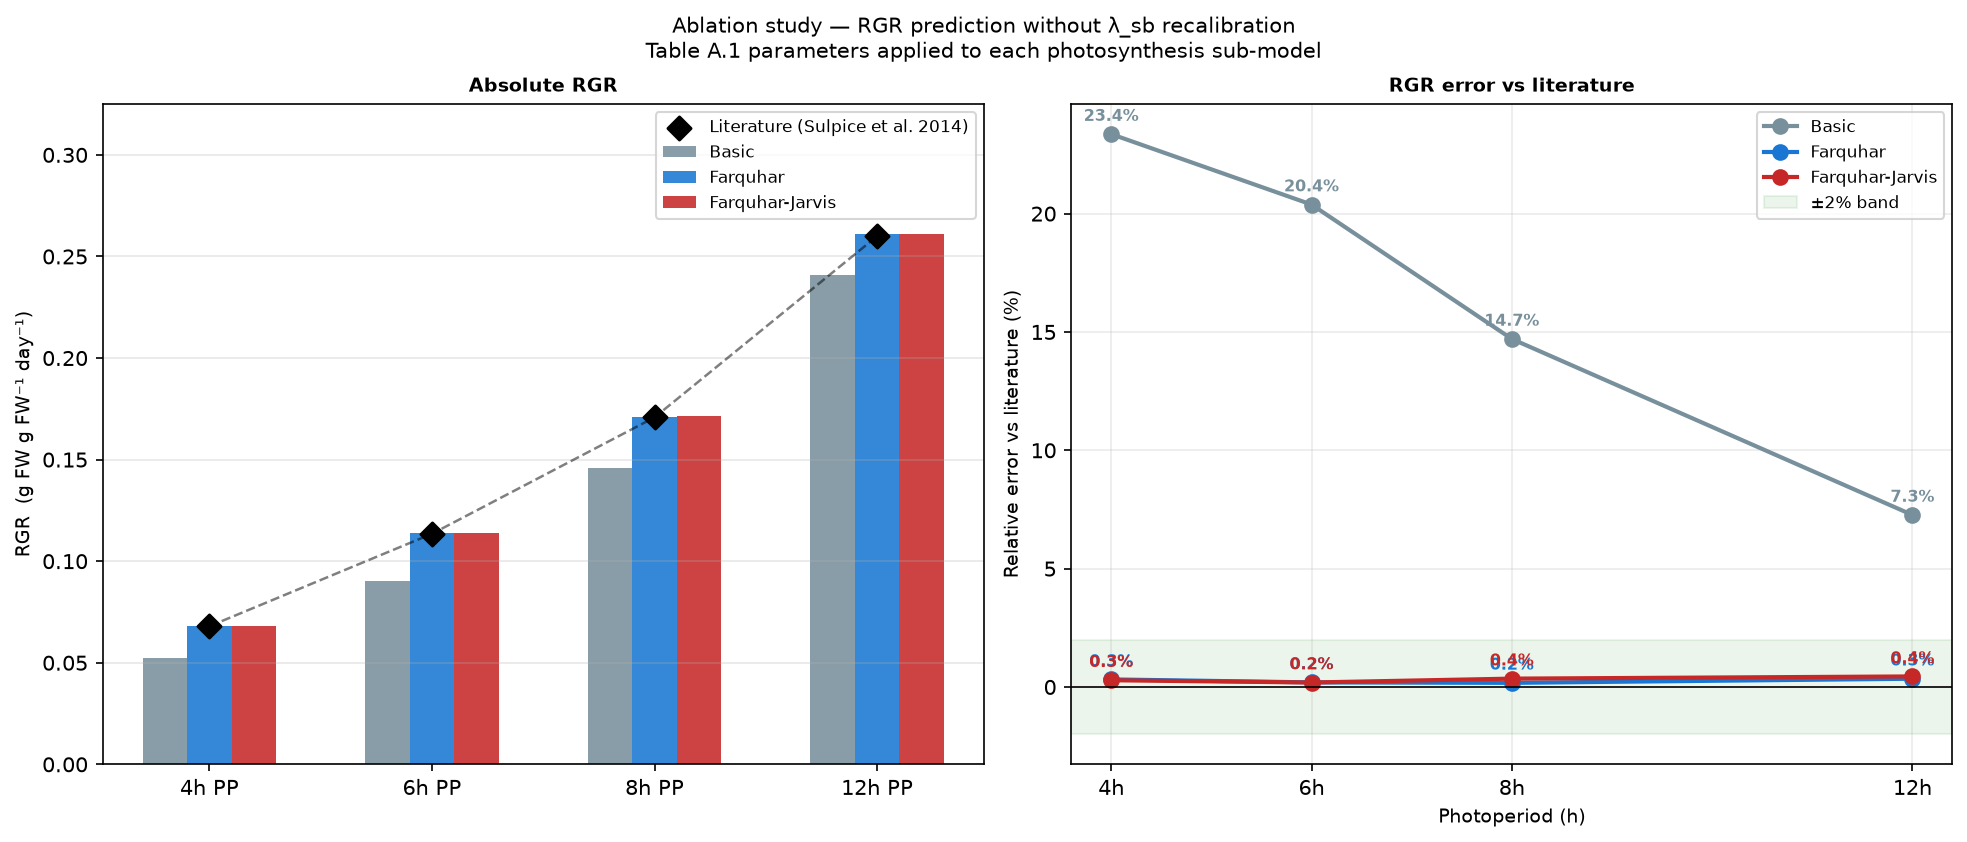
\includegraphics[width=\textwidth]{ablation_rgr.png}
\caption{Ablation study comparing RGR predictions obtained with the basic
carbon-input model, the Farquhar photosynthesis model, and the
Farquhar-Jarvis gas-exchange model. The left panel gives absolute RGR against
the literature targets, the right the relative error with the $\pm2\%$
acceptance band; $\lambda_{sb}$ is not recalibrated between sub-models, so all
three are run with the same Table~\ref{tab:param_values} values. Errors in the
right panel are plotted as \emph{magnitudes}: the basic model lies below the
target at every photoperiod, which the body text reports with the
corresponding negative sign. The basic model systematically
underestimates RGR, while the Farquhar and Farquhar-Jarvis variants remain
close to the literature targets.}
\label{fig:ablation_rgr}
\end{figure}

The basic model produced errors ranging from $-23.4\%$ under the 4 h
photoperiod to $-7.3\%$ under the 12 h photoperiod. This confirms that the
simplified carbon-input formulation was not sufficient to reproduce the
photoperiod-dependent RGR response. The Farquhar variant reduced the mean
absolute percentage error to below $0.3\%$. The Farquhar-Jarvis variant did
not substantially improve reported RGR relative to the Farquhar-only variant,
because the RGR target was already closely matched. Its contribution is instead
to expose the model to environmental drivers through stomatal regulation, which
is evaluated further in the sensitivity analyses.

% ------------------------------
\subsection{Global sensitivity of RGR}

All Sobol' indices reported here were recomputed after the sampling-design
defect described in Section~\ref{sec:sa_design} was corrected, and with the
analytic gas-exchange solver of Eq.~\eqref{eq:ci_quadratic}; they supersede
the values obtained with the original design, and the ranking changes. The
total-order analysis shows that RGR variability is dominated by the two
nutrient uptake capacity parameters, maximum phosphorus uptake $I_{P,\max}$
and maximum nitrogen uptake $I_{N,\max}$, followed by the respiration
frequency $r_m$ and then by the photosynthetic capacities $V_{c\max}$ and
$J_{\max}$, with leaf water potential $\psi_w$ and ambient CO$_2$ close
behind (Table~\ref{tab:dominant_sobol_parameters},
Fig.~\ref{fig:sobol_heatmap}).

\begin{table}[!htbp]
\centering
\caption{Dominant parameters ranked by mean Sobol' total-order index across
photoperiods. The table provides a compact global-sensitivity summary for the
RGR output.}
\label{tab:dominant_sobol_parameters}
\begin{tabular}{@{}rlrrrrrrr@{}}
\toprule
& Parameter & 4 h & 6 h & 8 h & 12 h & $\bar S_T$ & $\bar S_1$ & $\bar S_T-\bar S_1$ \\
\midrule
1  & $I_{P,\max}$         & 0.38 & 0.49 & 0.53 & 0.52 & 0.481 & 0.225 & 0.256 \\
2  & $I_{N,\max}$         & 0.46 & 0.41 & 0.40 & 0.25 & 0.378 & 0.093 & 0.285 \\
3  & $r_m$                & 0.46 & 0.37 & 0.34 & 0.22 & 0.348 & 0.028 & 0.320 \\
4  & $V_{c\max}$          & 0.21 & 0.21 & 0.22 & 0.31 & 0.238 & 0.039 & 0.199 \\
5  & $C_a$                & 0.24 & 0.17 & 0.18 & 0.26 & 0.211 & 0.042 & 0.169 \\
6  & $J_{\max}$           & 0.21 & 0.20 & 0.20 & 0.23 & 0.211 & 0.019 & 0.192 \\
7  & $\psi_w$             & 0.15 & 0.15 & 0.14 & 0.19 & 0.155 & 0.043 & 0.113 \\
8  & PAR$_{\max}$         & 0.13 & 0.13 & 0.13 & 0.19 & 0.147 & 0.018 & 0.130 \\
9  & $T$                  & 0.10 & 0.06 & 0.08 & 0.09 & 0.081 & 0.017 & 0.064 \\
10 & RH                   & 0.09 & 0.03 & 0.06 & 0.07 & 0.063 & 0.022 & 0.041 \\
11 & $P_{\mathrm{soil}}$  & 0.06 & 0.05 & 0.08 & 0.05 & 0.059 & 0.020 & 0.040 \\
12 & $N_{\mathrm{soil}}$  & 0.06 & 0.04 & 0.04 & 0.03 & 0.042 & 0.011 & 0.032 \\
13 & $\lambda_{sb}$       & 0.05 & 0.02 & 0.05 & 0.04 & 0.040 & 0.023 & 0.017 \\
14 & $k_{in}$             & 0.00 & 0.02 & 0.01 & 0.01 & 0.010 & 0.002 & 0.008 \\
15 & $s(0)$               & 0.00 & 0.02 & 0.01 & 0.01 & 0.009 & 0.002 & 0.007 \\
16 & $B(0)$               & 0.00 & 0.00 & 0.00 & 0.00 & 0.001 & 0.001 & 0.001 \\
\bottomrule
\end{tabular}
\end{table}

The full set of sixteen dimensions is listed rather than a top-ten subset,
because the indices that are near zero are themselves a result: the initial
conditions and both soil-content drivers contribute almost nothing to RGR
variance over the ranges of Appendix~\ref{app:sensitivity_params}, and
reporting only the dominant parameters would leave that unstated. All sixteen
interaction shares are non-negative in the recomputed design, in contrast to
the earlier estimates; the Saltelli estimator's total-order form is not
constrained to dominate the first-order term at finite $n$, and indices are
reported unclipped throughout, since clipping would misrepresent precision at this sample
size.

\begin{figure}[htbp]
\centering
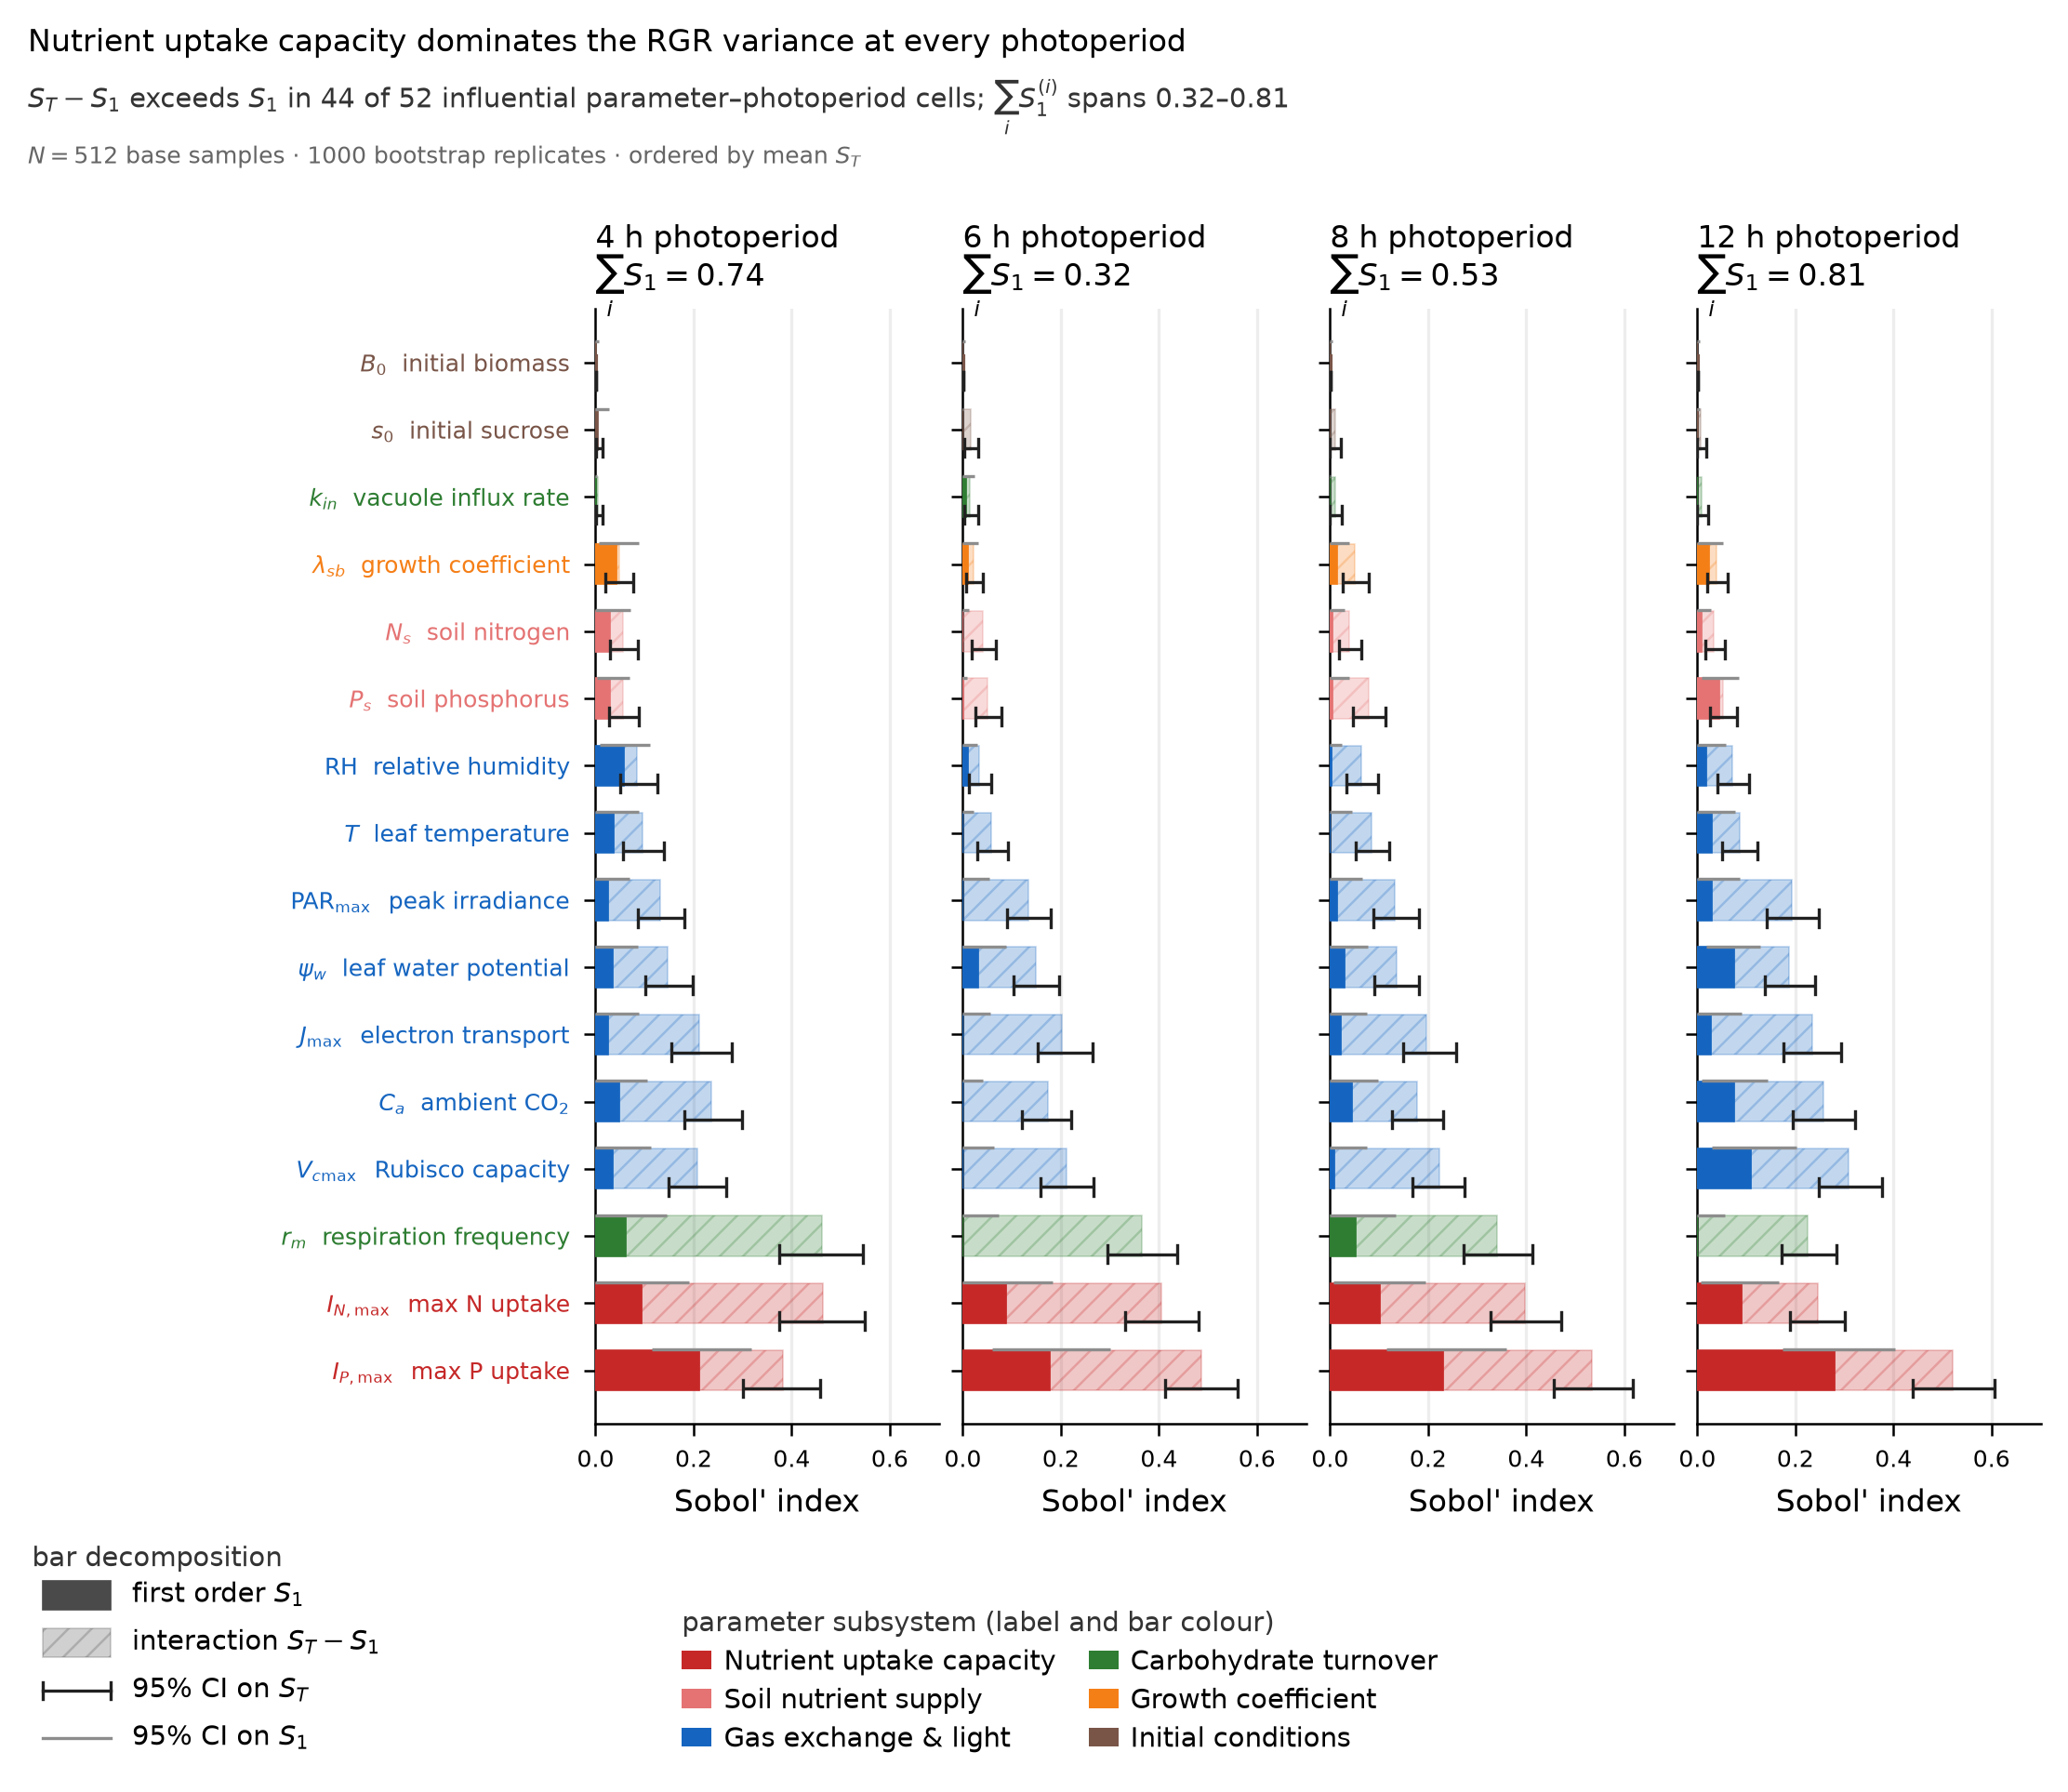
\includegraphics[width=0.82\textwidth]{sensitivity_heatmap.png}
\caption{Sobol' variance decomposition of RGR under four photoperiod
treatments. For each parameter the bar shows the first-order index $S_1$ (solid)
and the interaction remainder $S_T - S_1$ (hatched), with bootstrap $95\%$
confidence intervals from $1000$ resamples of the base rows; parameters are
ordered by mean total-order index across photoperiods. The interaction remainder
exceeds the first-order index in 44 of the 52 influential
parameter-photoperiod cells (9 of 16 parameters at 4~h, 16 of 16 at 6 and 8~h,
13 of 16 at 12~h), which is the central feature of the decomposition. Two reporting conventions should be noted. Indices are given
unclipped: the Saltelli total-order estimator is not constrained to dominate
$S_1$ at finite sample size, so where the estimator returns $S_1 > S_T$ within
bootstrap noise the solid segment is drawn clamped at $\min(S_1, S_T)$ while the
plotted intervals remain unclamped. The base design is two independent
Latin-hypercube samples rather than a split low-discrepancy sequence, for the
reason established in Section~\ref{sec:results_estimator}; the design actually
used is recorded in every output file.}
\label{fig:sobol_heatmap}
\end{figure}

The two nutrient uptake capacities remain dominant across the photoperiod
range but respond to it in opposite directions: $I_{P,\max}$ rises with day
length ($S_T = 0.38$ at 4~h to $0.52$ at 12~h, peaking at $0.54$ at 8~h),
whereas $I_{N,\max}$ declines monotonically from $0.46$ at 4~h to $0.25$ at
12~h. The respiration frequency shows the same decline, from $0.46$ to
$0.22$. The declining pair is consistent with a
shift in what limits growth as the photoperiod lengthens: under short days
the plant is carbon-limited, so the parameters governing the losses from and
the demands on a scarce carbohydrate pool matter most, while under long days
carbon is less scarce and the assimilation capacities $V_{c\max}$, $J_{\max}$
and the light and CO$_2$ supply gain influence --- $V_{c\max}$ rises from
$0.21$ at 4~h to $0.31$ at 12~h, $J_{\max}$ from $0.20$ at 8~h to $0.23$ at
12~h, and PAR$_{\max}$ from $0.13$ to $0.19$.
Leaf water potential acts in the opposite direction to $I_{N,\max}$, rising
from $0.15$ to $0.19$, which is expected if its effect is mediated by
stomatal limitation of an assimilation flux whose importance itself grows
with day length. All values in this paragraph are the total-order indices of
Table~\ref{tab:dominant_sobol_parameters}, i.e.\ the recomputed design of
Section~\ref{sec:results_estimator}.

The most informative column of Table~\ref{tab:dominant_sobol_parameters} is
the last. For fifteen of the sixteen parameters --- all but $B(0)$, whose
indices are indistinguishable from zero --- the interaction share
$\bar S_T-\bar S_1$ exceeds the first-order index, and for the most extreme
cases it does so by an order of magnitude: $r_m$ has $\bar S_1 = 0.028$ against
$\bar S_T = 0.348$, and $J_{\max}$ has $\bar S_1 = 0.019$ against
$\bar S_T = 0.211$. Resolved by photoperiod rather than averaged over them, the
interaction remainder exceeds the first-order index in 44 of the 52 influential
parameter-photoperiod cells, and the margin is thinnest at the $4$~h photoperiod
(9 of 16 parameters) --- the averaged column overstates the uniformity of the
effect, and the per-photoperiod count is the honest statement of it. Little of
the RGR variance is attributable to any parameter acting alone. This is the quantitative signature of the coupling
the model is built around, and it has a methodological consequence worth
stating: a one-at-a-time sensitivity analysis of this model would have found
$r_m$ and $J_{\max}$ nearly inert, and would have been wrong. The
aggregate figures make the point compactly: summed over the sixteen
dimensions, the first-order indices account for only $0.32$ to $0.81$ of the
RGR variance depending on photoperiod, while the total-order indices sum to
$2.36$ to $2.59$ against unity for a purely additive model. Between $19\%$ and
$68\%$ of the variance is therefore unexplained by main effects, and is
carried by interactions of second and higher order. The width of that range is
itself informative: the main-effect share is smallest at the $6$~h photoperiod,
where the plant operates closest to the carbon-limited transition and the
parameters act most strongly through one another.

The parameters associated with soil nutrient content, initial sucrose,
initial biomass and vacuolar influx have low total-order indices over the
analysed ranges. Two of these deserve comment rather than dismissal. The
calibrated growth coefficient $\lambda_{sb}$ has $\bar S_T = 0.040$, which is
not a contradiction of the calibration result of
Section~\ref{sec:results_verification}: $\lambda_{sb}$ sets the level of the
growth response and the calibration exploits exactly that, but over the
$\pm70\%$ range sampled here it contributes little to the \emph{variance} of
RGR relative to parameters that act multiplicatively through the whole
carbon chain. Sensitivity and identifiability are different questions, and a
low $S_T$ does not license fixing a parameter that a calibration depends on.
The vacuolar influx $k_{in}$ has $\bar S_T = 0.010$, consistent with the
equilibrium argument of Section~\ref{sec:carbohydrates}: the vacuole
redistributes sucrose in time without changing the integrated carbon
available, so it shapes the diel trajectory much more than the 35-day growth
integral used as the output metric here.

% ------------------------------
\subsection{Verification of the sensitivity estimator}
\label{sec:results_estimator}

The indices above are only as trustworthy as the estimator that produced
them, and in the originally submitted version they were not trustworthy.
The Saltelli estimator requires two \emph{independent} base samples,
$\mathbf{A}$ and $\mathbf{B}$. The implementation built them by drawing one
Sobol' sequence of length $2n$ and splitting it into halves. Successive
blocks of a low-discrepancy sequence are constructed to fill the gaps left by
earlier blocks and are therefore strongly dependent: at $d = 16$ the
column-wise correlation between the two halves reached $1.0000$. The
estimator then differences two nearly identical matrices, and the variance
decomposition collapses.

Against the Ishigami function of Eq.~\eqref{eq:ishigami}, for which the
indices are known in closed form ($S_1 = [0.3139, 0.4424, 0]$,
$S_T = [0.5576, 0.4424, 0.2437]$), the published design does not converge at
all: as $n$ grows from $256$ to $16384$ the mean absolute error over eight
seeds moves from $0.31$ to $0.30$ for $S_1$ and from $0.29$ to $0.30$ for
$S_T$ --- no dependence on sample size --- and $S_1$ for $x_1$ is estimated as
exactly $0.000$ against a true $0.3139$. A correct column split of a single
$n\times 2d$ sequence converges over the same range, MAE($S_1$) falling from
$0.034$ to $0.0007$; two independent Latin-hypercube samples converge at
approximately $n^{-1/2}$, from $0.055$ to $0.006$. Merely reseeding the
Sobol' sampler and calling it twice does \emph{not} fix the problem: the error
falls from $0.042$ to $0.021$ and then stops at that floor, because reseeding
this sampler does not yield an independent set. Since the available sampler
supports at most 16 dimensions and this problem has $d = 16$, the preferred
$2d = 32$ column split is unavailable, and the adaptive design of
Section~\ref{sec:sa_design} falls back to the Latin-hypercube construction;
which design was used is recorded in a \texttt{base\_design} column of every
Sobol' output file.

The defect had already announced itself in our own convergence study, and was
misread as noise. For the maximum nitrogen uptake capacity $I_{N,\max}$, $S_T$ was
$0.44$ at $n = 512$, $0.15$ at $n = 2048$, and $0.44$ again at $n = 4096$,
with a bootstrap $95\%$ interval at $n = 2048$ of $[0.128, 0.174]$ that
excluded the $n = 4096$ estimate. Across ten replicate designs the spread at
$n = 2048$ was \emph{wider} than at $n = 512$, and the ratio of across-design
standard deviation to within-design bootstrap standard error rose from $1.10$
at $n = 512$ to $4.64$ at $n = 2048$. An estimator whose variance grows with
sample size is misspecified, not noisy, and that diagnostic is available
without any external benchmark.

With the corrected design the across-design standard deviation of $S_T$ falls
as it should: averaged over the sixteen dimensions at the 12~h photoperiod it
is $0.0347$ at $n = 128$, $0.0177$ at $n = 512$ and $0.0074$ at $n = 2048$,
close to the $n^{-1/2}$ rate. At $n = 512$ the across-design standard
deviation and the within-design bootstrap standard error now agree, with a
mean ratio of $0.88$ (range $0.55$ to $1.25$) over the sixteen dimensions,
against $1.10$ rising to $4.64$ before the fix. Both uncertainties are
reported, because they measure different things: a bootstrap resamples within
one fixed design and is blind to error contributed by the design itself, so
the replicate-design spread is the quantity that would have caught this
defect. The Morris screening required no recomputation --- it draws
trajectory base points from an independent pseudo-random generator, as
\citet{Morris1991} specifies, and never touches the affected sampler.

\begin{figure}[htbp]
\centering
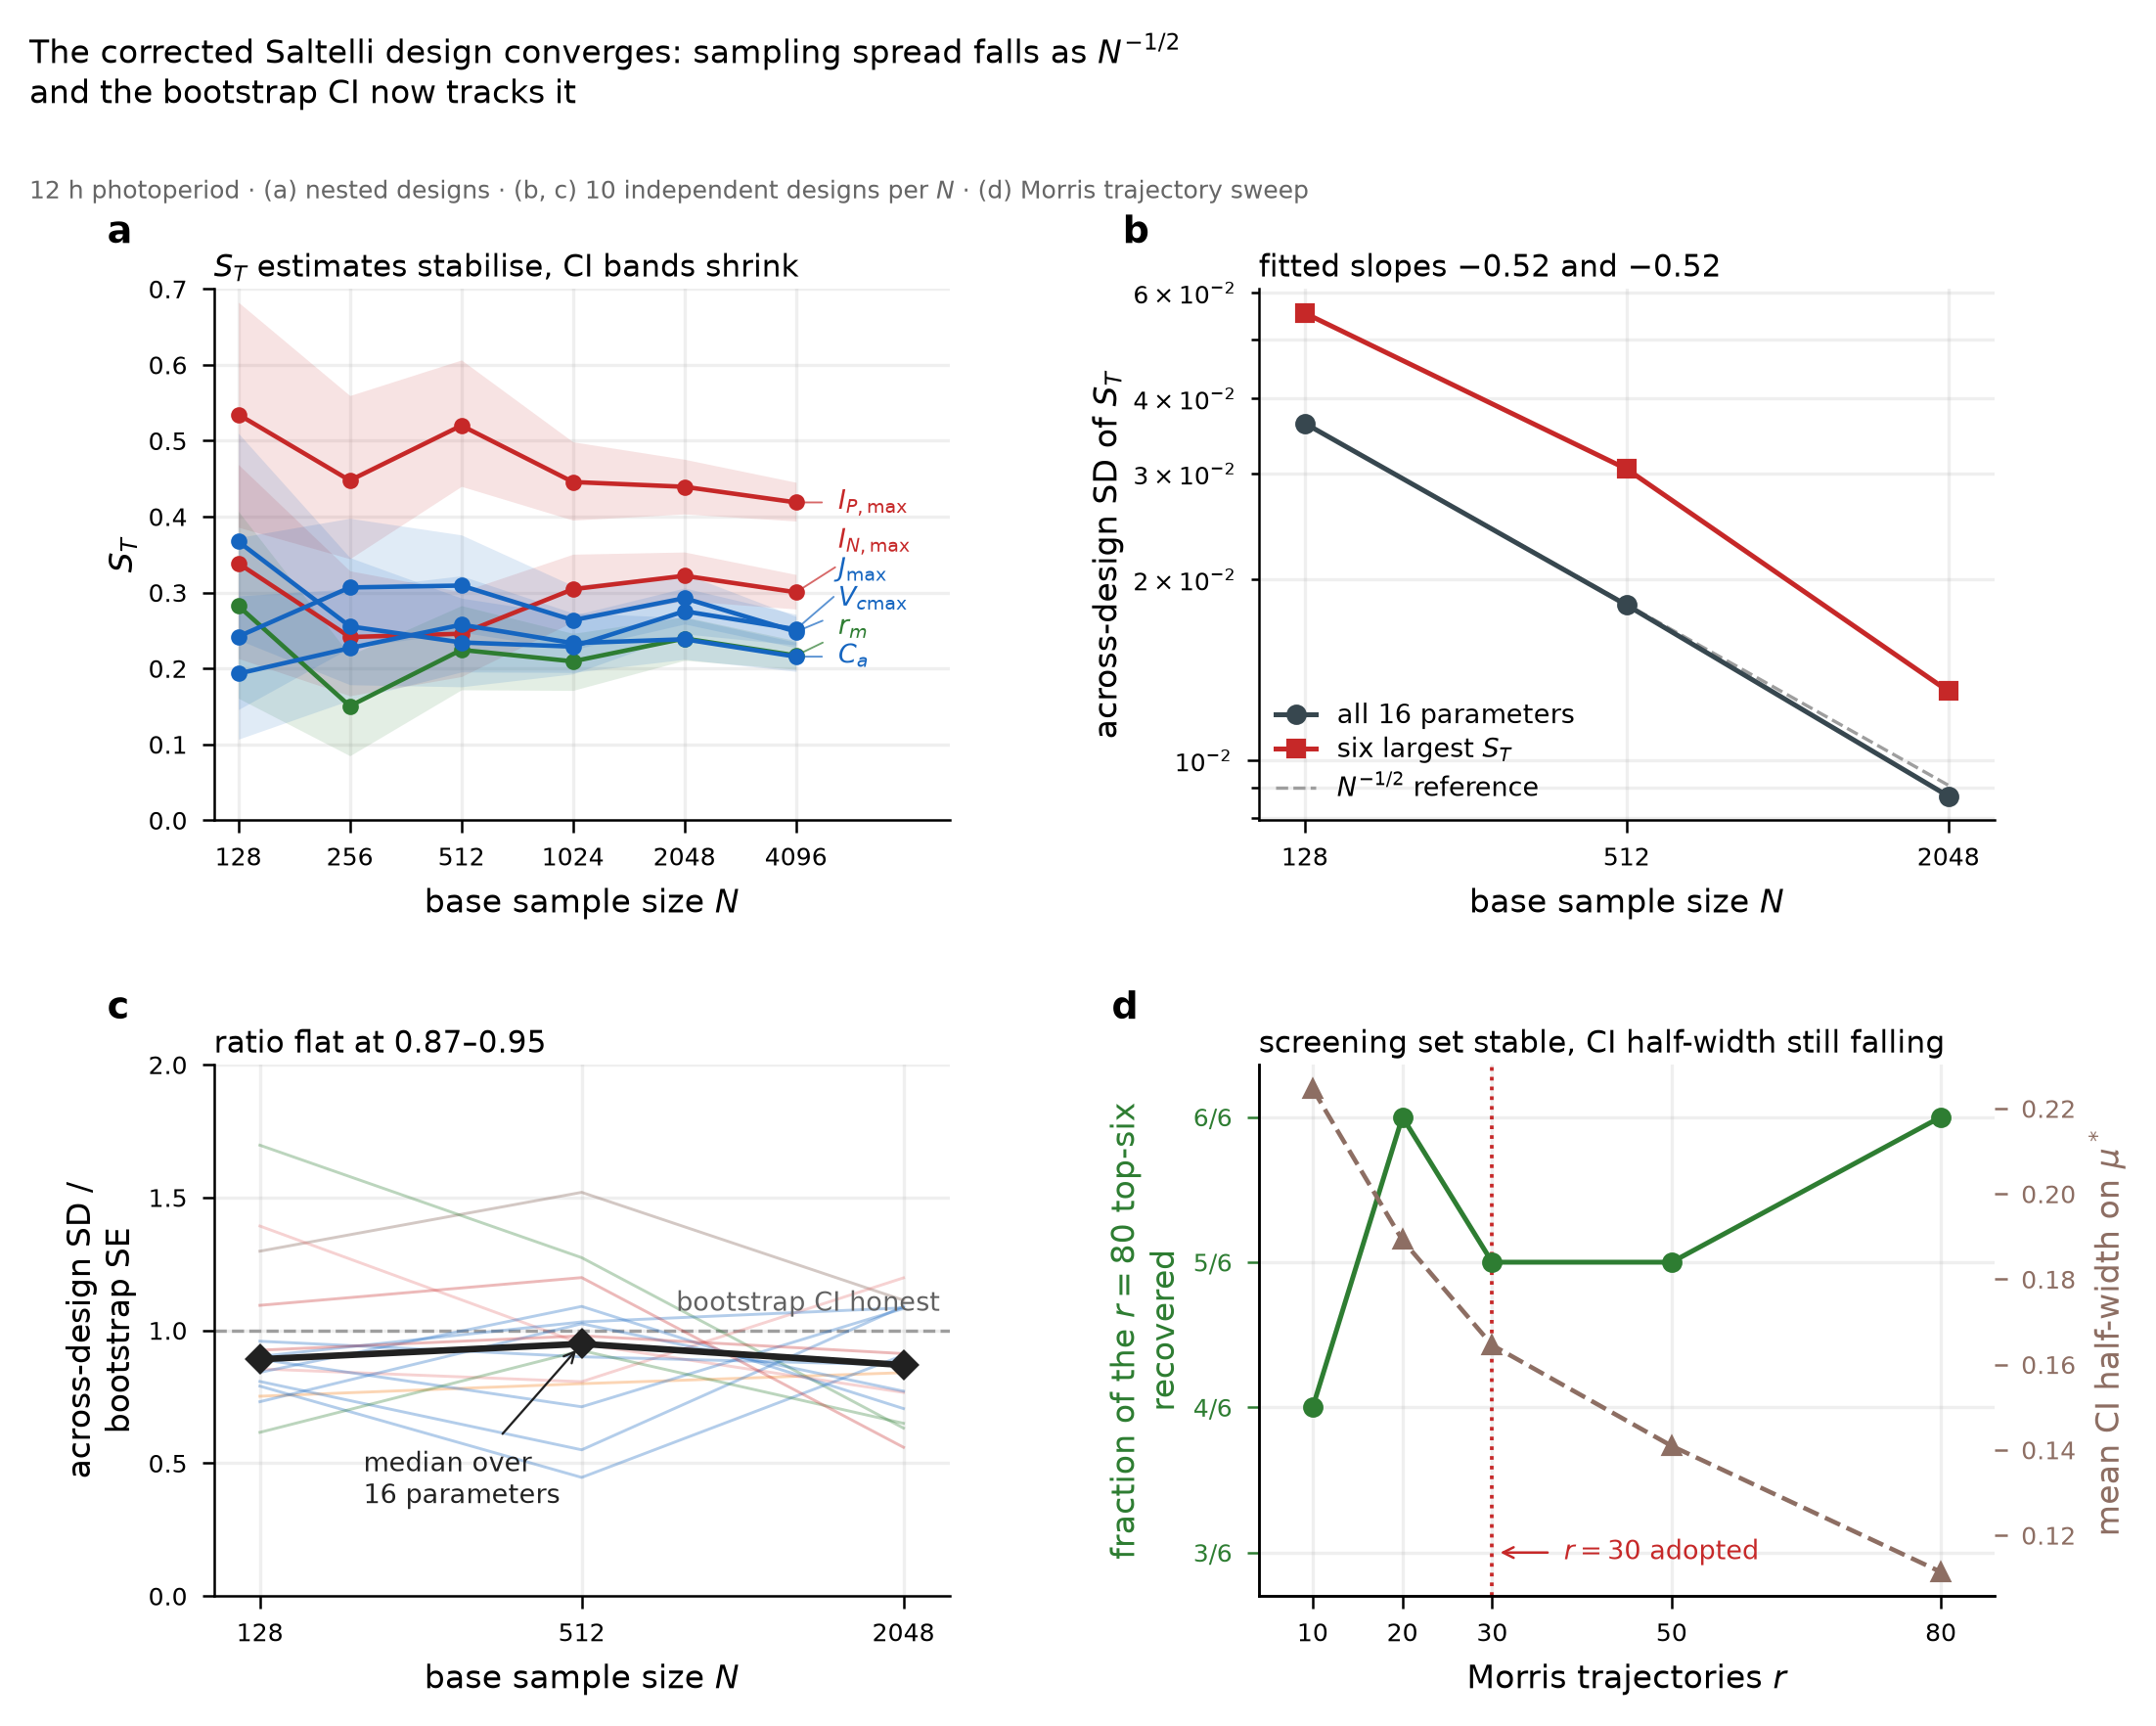
\includegraphics[width=\textwidth]{sensitivity_convergence.png}
\caption{Convergence of the sensitivity estimators with the corrected base
design, 12~h photoperiod. (a) Total-order indices $S_T$ against base sample size
$N$ for the six leading dimensions over nested designs, with bootstrap $95\%$
bands; the bands shrink steadily and the estimates settle to within $0.03$ of
their $N = 4096$ values from $N \approx 1024$ upward (to within $0.10$ at
$N = 512$).
(b) Across-design standard deviation of $S_T$ over ten independent designs per
$N$, for all sixteen dimensions and for the six largest, on logarithmic axes
with an $N^{-1/2}$ reference; the fitted slopes are $-0.52$ in both cases, in
contrast to the pre-fix behaviour in which the spread grew with $N$. (c) Ratio of
across-design standard deviation to within-design bootstrap standard error, per
parameter and as a median; the ratio is flat at $0.87$--$0.95$, so the bootstrap
interval is now an honest measure of total estimator uncertainty, against a
ratio rising to $4.64$ before the fix. (d) Morris trajectory sweep: the fraction
of the $r = 80$ top-six screening set recovered at each $r$ (left axis) and the
mean bootstrap confidence half-width on $\mu^*$ (right axis). The half-width
falls monotonically with $r$ ($0.225$, $0.189$, $0.165$, $0.141$, $0.111$ at
$r = 10, 20, 30, 50, 80$), while the screened-in set is within one member of
the $r = 80$ set from $r = 20$ upward and does not settle onto a single
composition at any $r$ tested ($4$, $6$, $5$, $5$, $6$ of six recovered).
That is why $r = 30$ is adopted for screening only and no rank ordering is read
from it: the leading $\mu^*$ values cluster within $0.34$--$0.51$ at $r = 30$
and their relative order remains unstable, so Morris is used here to separate
influential from negligible parameters and the variance decomposition is used
for attribution.}
\label{fig:sensitivity_convergence}
\end{figure}

% ------------------------------
\subsection{Morris screening and interaction behaviour}

Morris screening supported the Sobol' ranking and provided additional evidence
about nonlinear and interaction-driven effects. Parameters with high
$\mu^\ast$ had large mean elementary effects, while parameters with high
$\sigma$ indicated nonlinear responses, interactions, or photoperiod-dependent
behaviour (Fig.~\ref{fig:morris_screening}).

\begin{figure}[htbp]
\centering
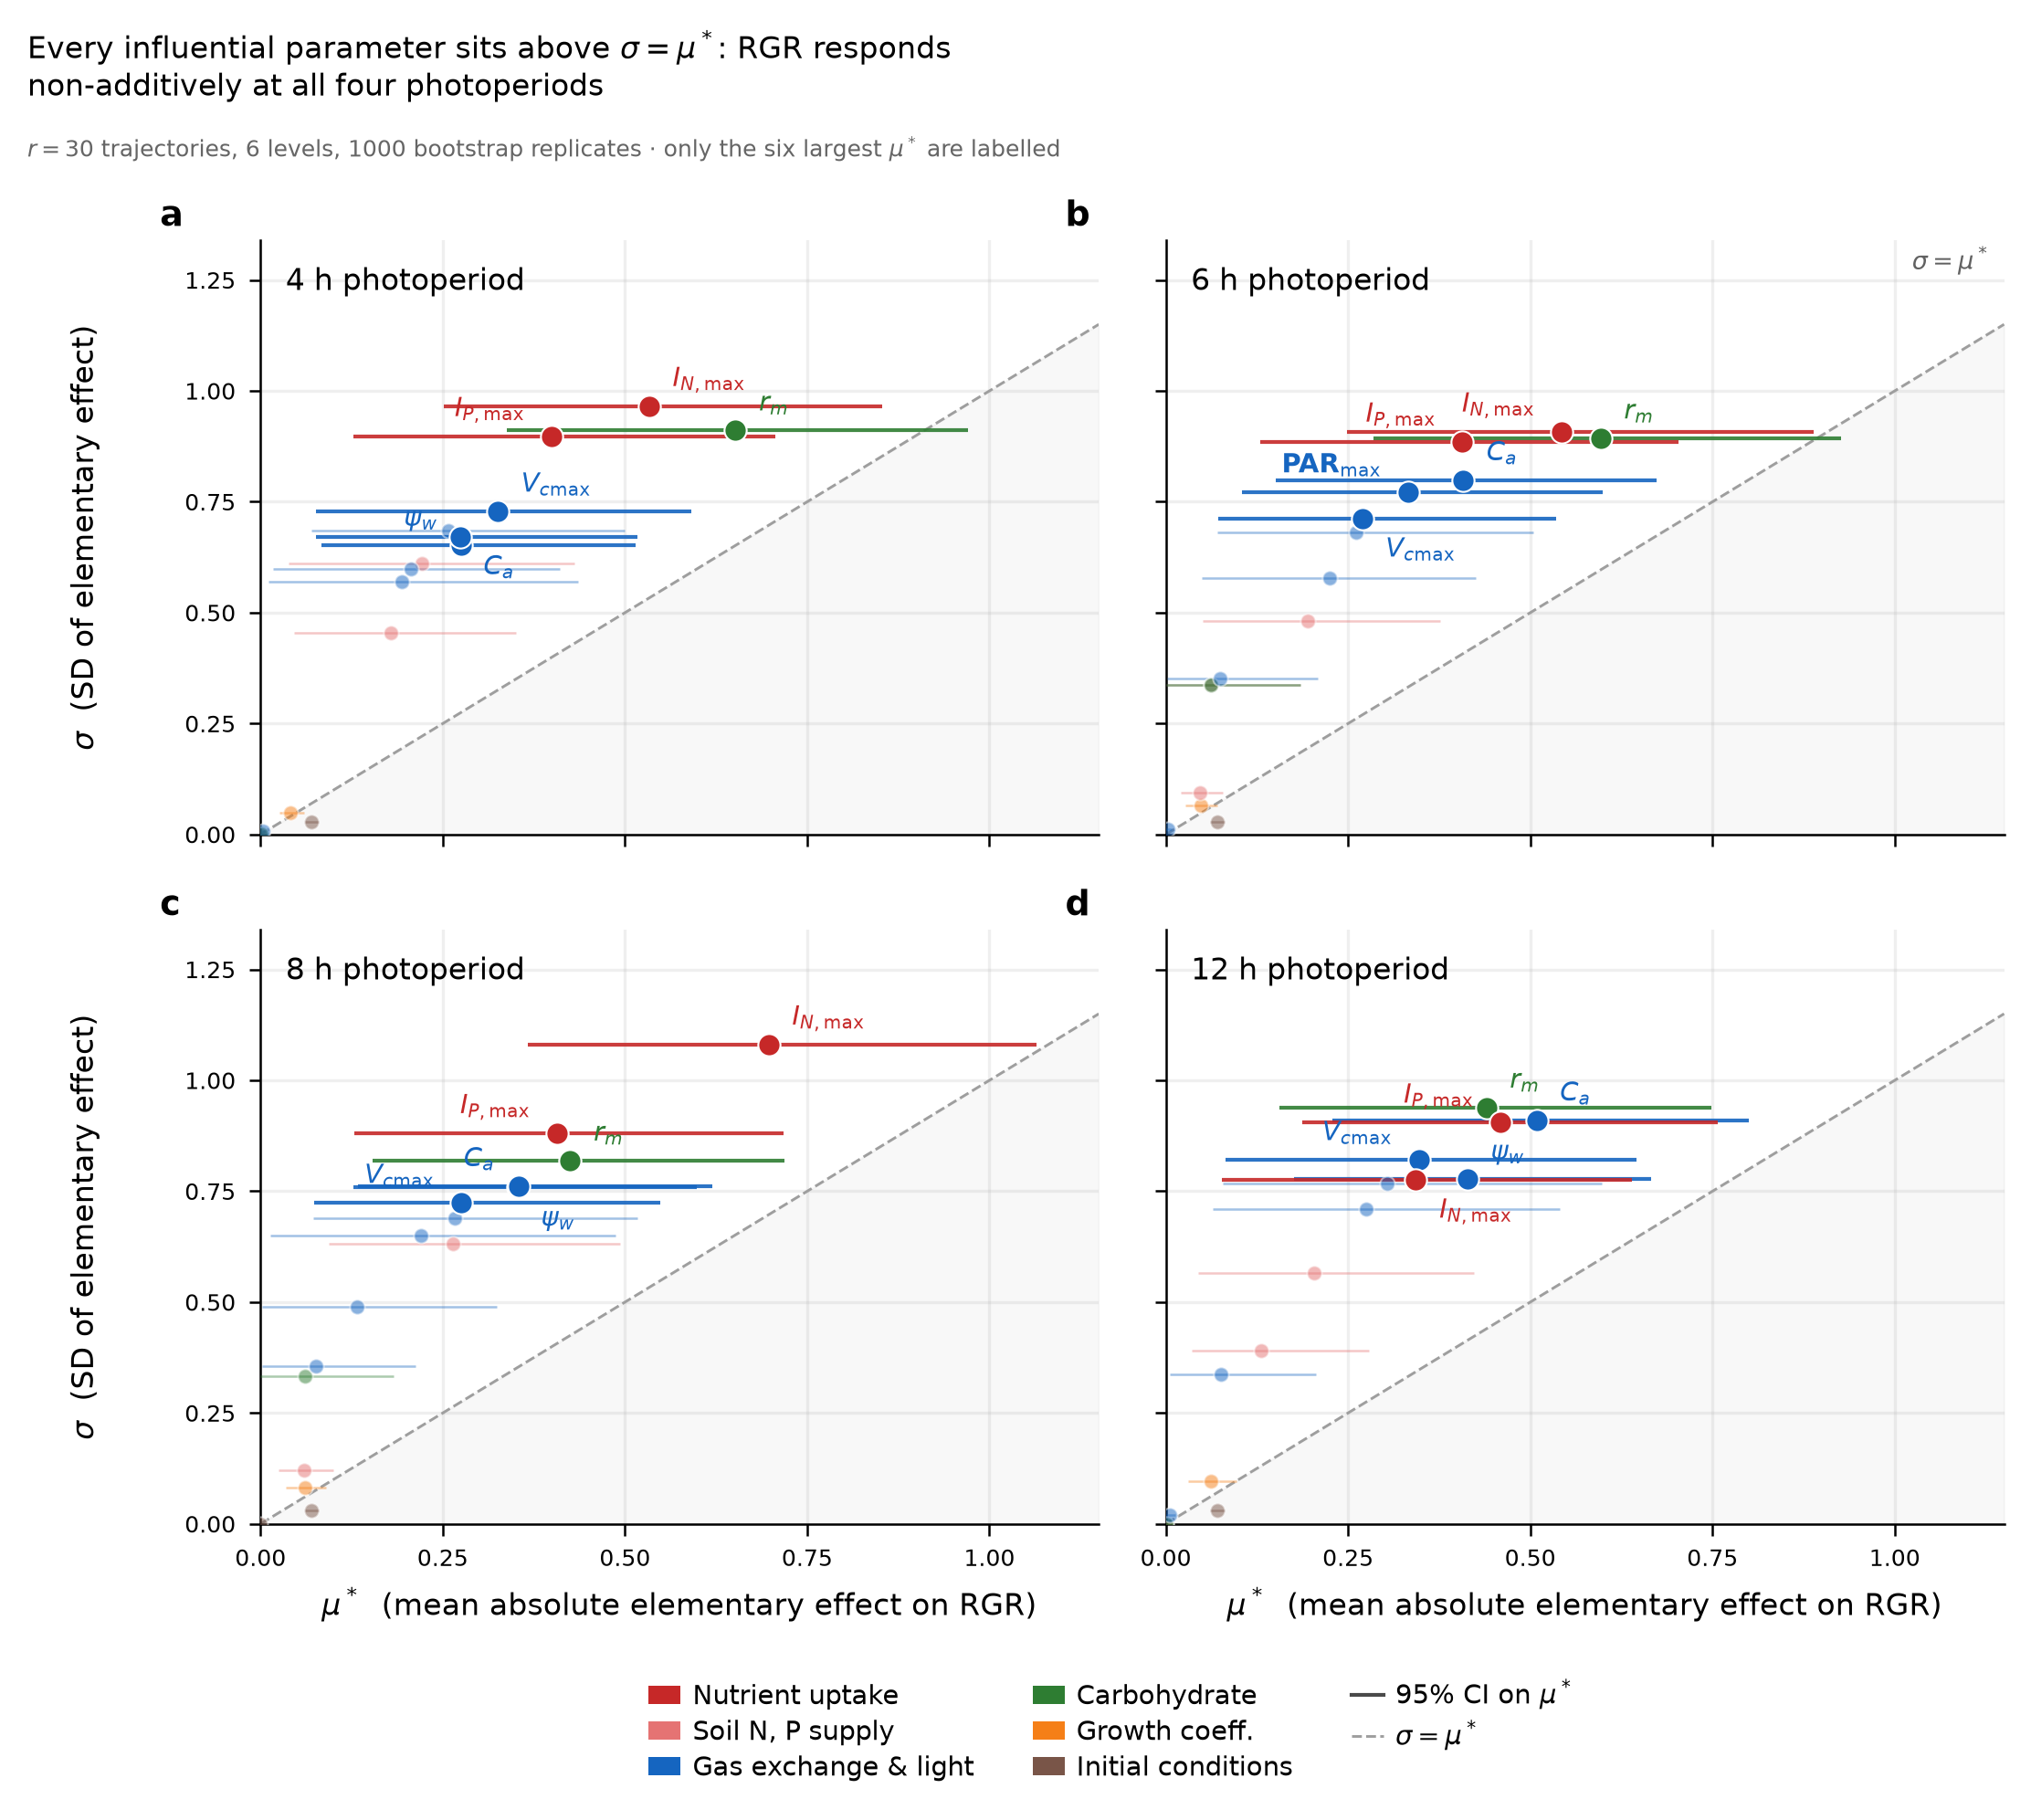
\includegraphics[width=\textwidth]{morris_scatter.png}
\caption{Morris screening of the RGR output at the 4, 6, 8 and 12~h
photoperiods (panels a--d); $r = 30$ trajectories on $6$ levels, with $95\%$
bootstrap confidence bars on $\mu^*$ from $1000$ replicates and colour by
parameter subsystem. High $\mu^\ast$ indicates a large mean absolute elementary
effect and high $\sigma$ nonlinear or interaction-driven behaviour; the dashed
diagonal is $\sigma = \mu^*$, and every parameter with appreciable $\mu^*$ lies
above it at all four photoperiods. Only the six largest $\mu^*$ are labelled.}
\label{fig:morris_screening}
\end{figure}

The nutrient uptake capacity parameters appear in the high-$\mu^\ast$,
high-$\sigma$ region, indicating both strong influence and nonlinear or
interaction-driven behaviour. Gas-exchange and light-related parameters also
show substantial effects, particularly under longer photoperiods. The
agreement with the Sobol' ranking is a meaningful check rather than a
restatement, because the two methods share no sampling machinery: Morris draws
its trajectory base points from an independent pseudo-random generator and was
therefore unaffected by the design defect of
Section~\ref{sec:results_estimator}, so it provides a ranking obtained
without the corrected Saltelli estimator. Together the two analyses show that
RGR is not controlled by a single fitted growth coefficient, but by the
combined effect of nutrient uptake capacity, respiration, photosynthetic
capacity, water status and photoperiod-dependent carbon availability.

% ------------------------------
\subsection{Local response diagnostics}

The one-at-a-time (OAT) parameter sweeps and parameter-pair response surfaces
are reported as local diagnostics, not as a ranking. They cannot serve as one
here: the interaction shares in
Table~\ref{tab:dominant_sobol_parameters} show that for fifteen of the
sixteen parameters most of the RGR variance arises from interactions, which an
OAT sweep holding all other parameters at nominal values cannot see. Their
value is in the shape of the response --- where it saturates, where it changes
sign, and how it depends on photoperiod --- which the variance decomposition
does not report.

\begin{figure}[htbp]
\centering
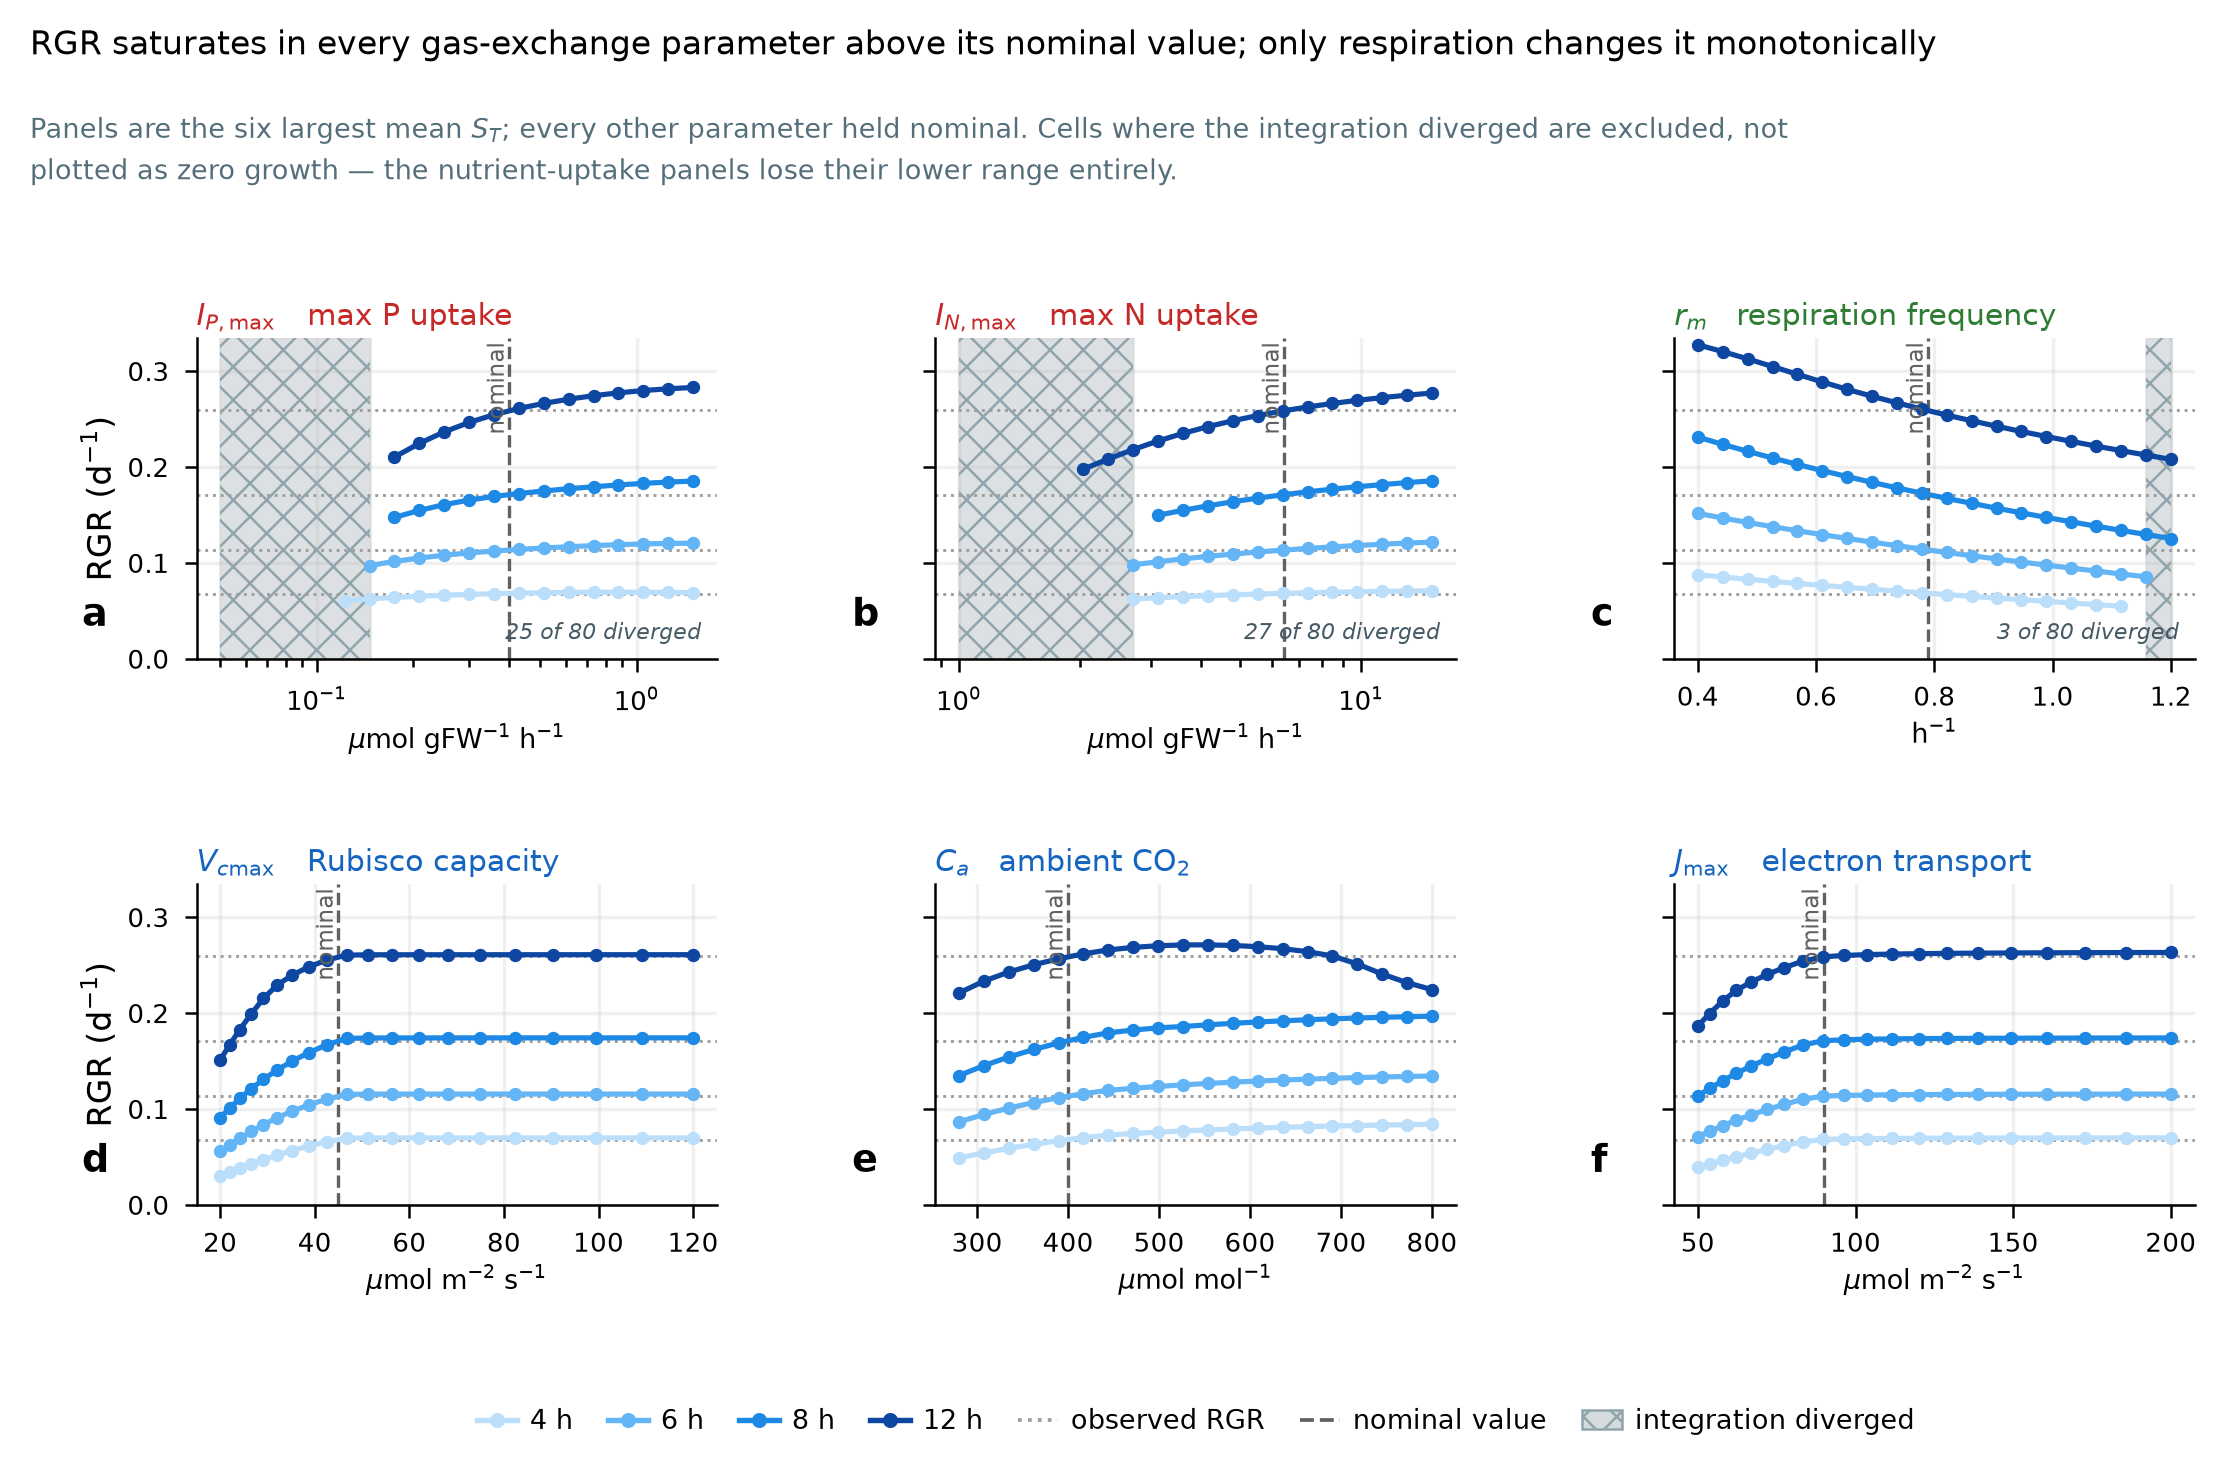
\includegraphics[width=\textwidth]{oat_sweep_main.png}
\caption{One-at-a-time parameter responses of relative growth rate at four
photoperiods. Panels show the six parameters with the largest mean total-order
Sobol' index $S_T$; every other parameter is held at its nominal value from
\texttt{config/default.config} (dashed vertical line). Dotted horizontal lines
mark the observed RGR of \citet{Sulpice2014} at the
corresponding photoperiod. Grey hatched bands mark sub-ranges in which the
integration diverged: in nutrient-limited parameter space the plant outgrows the
soil supply, the nutrient content crosses zero and the affinity equation reaches
its pole. These cells are excluded rather than plotted as zero growth --- a
distinction that matters, since all 55 zero-valued cells in the previously
reported sweep were divergences of this kind and none was genuine starvation.
Both nutrient-uptake capacities lose their lower range entirely. RGR saturates
above the nominal value in the capacity parameters, but not in ambient CO$_2$
(panel e), which peaks at $0.2713\ \mathrm{d^{-1}}$ near $554$~ppm and falls to
$0.2246\ \mathrm{d^{-1}}$ by $800$~ppm --- a non-monotone response, not a
plateau. Only respiration
frequency $r_m$ varies RGR monotonically across the whole admissible range.}
\label{fig:oat_sweep}
\end{figure}

The OAT sweeps (Fig.~\ref{fig:oat_sweep}) showed saturating responses for
nutrient uptake capacity,
photosynthetic capacity, water potential, and irradiance-related parameters.
Respiration frequency showed the expected negative effect on RGR: increasing
$r_m$ reduced growth. Environmental variables such as CO$_2$, temperature,
relative humidity, and PAR$_{\max}$ produced photoperiod-dependent responses,
supporting the interpretation that the Farquhar-Jarvis layer changes the
model behaviour beyond a prescribed carbon-input formulation.

\begin{figure}[htbp]
\centering
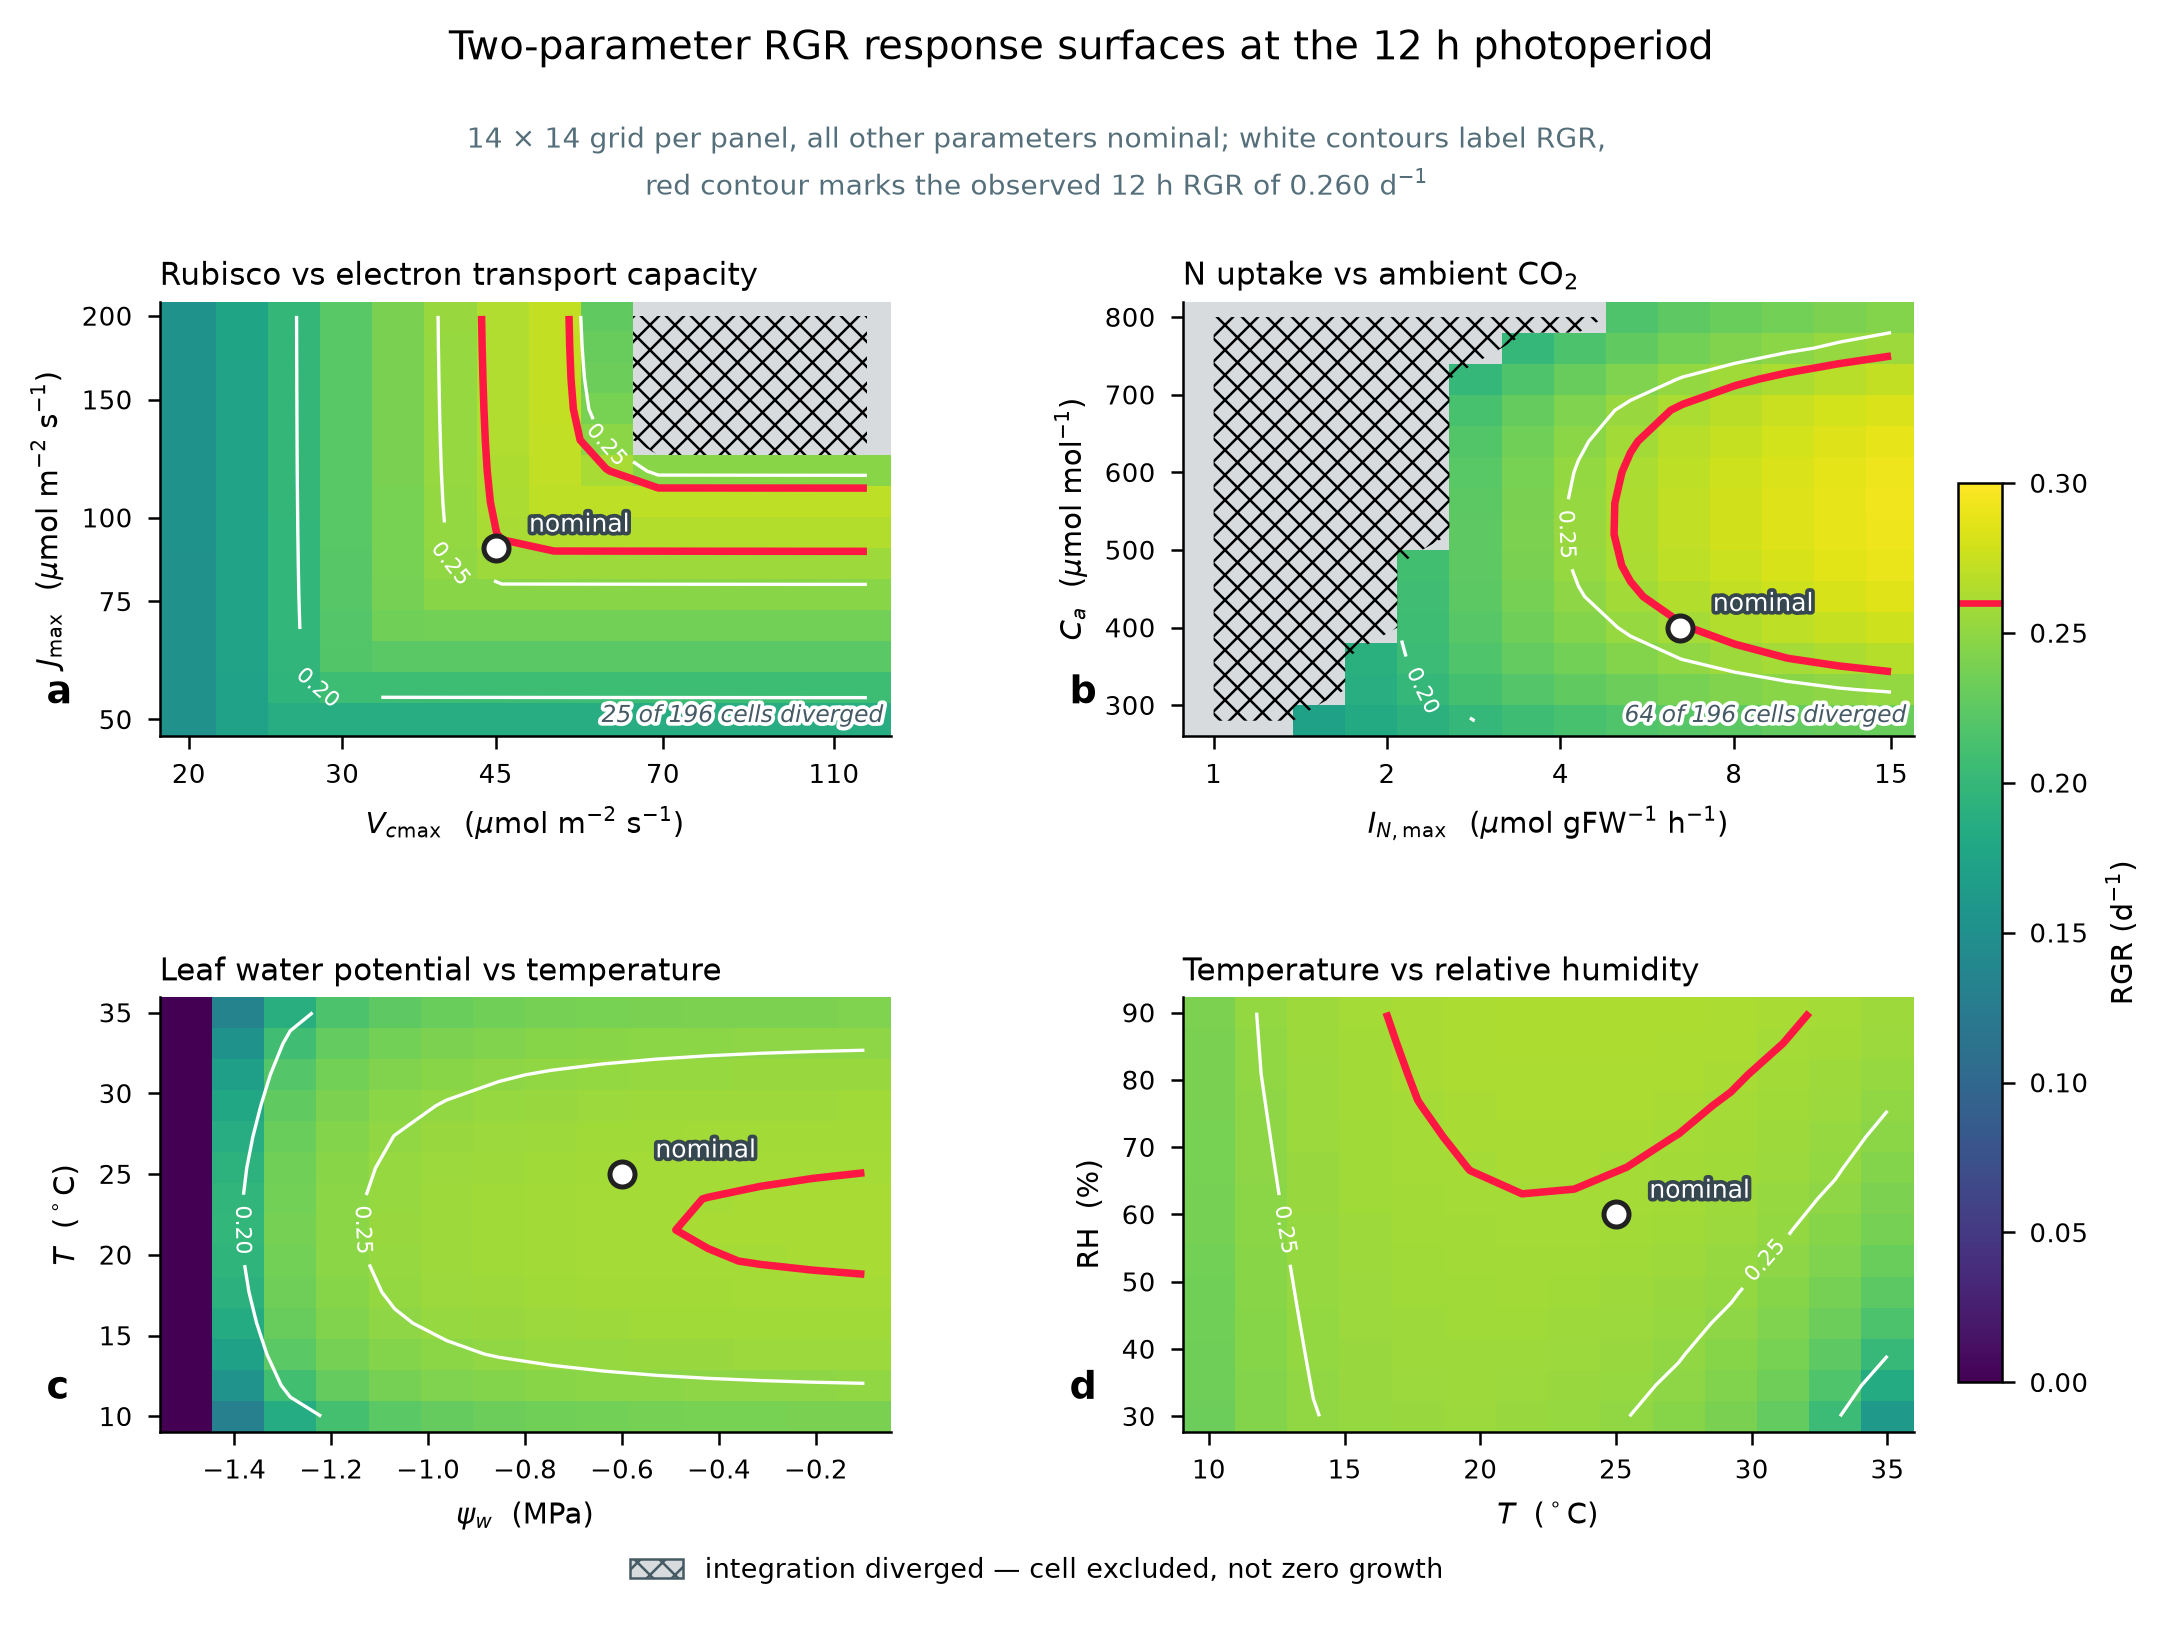
\includegraphics[width=\textwidth]{env_response_contours.png}
\caption{Two-parameter RGR response surfaces at the 12~h photoperiod,
$14\times14$ grid per panel, all other parameters at their nominal values.
White contours label RGR in d$^{-1}$; the red contour marks the observed 12~h
value of $0.260$~d$^{-1}$ \cite{Sulpice2014} and the white-filled marker the
nominal operating point. Grey hatched cells are excluded divergences, not zero
growth. (a) Rubisco and electron-transport capacity co-limit assimilation, and
the observed RGR is reached along an L-shaped locus that passes through the
nominal point. (b) Nitrogen uptake and ambient CO$_2$ trade off; below
$I_{N,\max} \approx 2\ \mu$mol~gFW$^{-1}$~h$^{-1}$ the run diverges over most
of the CO$_2$ range. (c) The dark column at $\psi_w = -1.5$~MPa is genuine
near-zero growth (RGR $\approx 10^{-4}$~d$^{-1}$), not a masked cell ---
stomatal closure, not integrator failure. (d) The temperature optimum shifts
upward with relative humidity, from about $20^{\circ}$C at $30\%$ to about
$23^{\circ}$C at $90\%$, and the observed-RGR contour is open toward high
humidity only: below about $60\%$ relative humidity the observed value is not
reached at any temperature.}
\label{fig:parameter_pair_surfaces}
\end{figure}

The two-parameter response surfaces (Fig.~\ref{fig:parameter_pair_surfaces})
confirm that interaction effects are strongest for pairs involving nutrient
uptake, water status, temperature, CO$_2$ and photosynthetic capacity, and they
add information the variance decomposition cannot carry. The contours are not
monotone ridges: the observed RGR is reached along an extended locus rather than
at a point, so the calibration problem is ill-conditioned in exactly the
directions the Sobol' interaction terms flag. Panel (c) also distinguishes two
outcomes that a variance-based index cannot: the near-zero growth at
$\psi_w = -1.5$~MPa is physiological stomatal closure, whereas the hatched
regions in (a) and (b) are integration failures, excluded rather than scored.
These surfaces are therefore consistent with the Sobol' and Morris results ---
the model response is dominated by the interaction of nutrient acquisition, gas
exchange, environmental forcing and photoperiod-dependent carbon availability
--- while making the shape of that interaction legible.


% ============================================================
\section{Discussion}
\label{sec:discussion}

\subsection{Principal findings and the role of the coupling}

The substantive result of this work is not the closeness of the fitted RGR
values but the behaviour of the coupled system, and the two must be separated
clearly. The calibration adjusts two coefficients per photoperiod against two
observations per photoperiod, so the reported mean absolute percentage error
of $0.24\%$ in RGR (Table~\ref{tab:rgr_validation_results}) is the
convergence residual of a bisection, not a predictive error; with eight
parameters and eight observations the fit has no degrees of freedom, and
tightening the tolerance drives the residual to zero. The out-of-sample test
gives the figures that do carry information. Across seven training/test splits,
a single photoperiod-independent parameter pair predicts held-out photoperiods
with a mean absolute percentage error of $28.5\%$, rising to $87\%$ in the
worst split (Table~\ref{tab:crossval}). The gap between $0\%$ and $28.5\%$
measures how much of the photoperiod response is carried by the calibrated
coefficients rather than by the simulated dynamics, and it is large.

The second cross-validated hypothesis sharpens that statement into something
more useful than a verdict. Allowing $\lambda_{sb}$ to vary linearly with
photoperiod --- one additional parameter, still photoperiod-independent in the
sense that no coefficient is refitted per treatment --- reduces the mean
held-out error from $28.5\%$ to $7.3\%$. The missing photoperiod dependence is
therefore not diffuse: it is close to an affine trend in the single coefficient
that converts night-time phloem loading into biomass. That is a specific
mechanistic gap. A plausible reading is that the model's night-time carbon
economy is missing a photoperiod-dependent efficiency --- longer nights impose
a longer period of remobilisation at lower rate, which in the reference
experiments is accompanied by adjustments in starch turnover that the fixed
$\lambda_{sb}$ cannot express. The splits also separate interpolation from
extrapolation cleanly: predicting the interior photoperiods from the endpoints
gives $4.5$--$8.5\%$ error, whereas predicting the short photoperiods from the
long ones gives $16.7$--$35.9\%$, so the model's photoperiod response degrades
mainly outside the calibrated range rather than uniformly. We report it because the alternative --- presenting a saturated fit as
a validation --- is a failure mode common enough in simulation studies to be
worth naming, and because a reader cannot detect it from the reported errors
alone.

What the model does reproduce without per-photoperiod adjustment is the
internal carbohydrate behaviour. Transient starch accumulated in the light
phase and was drawn down in the dark phase in all scenarios, with starch
nRMSE between $0.128$ and $0.192$ (Table~\ref{tab:sugar_starch_validation_results}),
with the observed near-linear nocturnal depletion arising from the structure
of Eq.~\eqref{eq:starch_degradation} rather than being fitted: the
degradation rate is the degradable reserve latched at dusk divided by the
night length, modulated by sucrose status, so depletion is paced to the night
irrespective of how much starch was accumulated during the day. The correct statement is
therefore that the shape is a consequence of the formulation and the
photoperiod forcing, not of any parameter tuned to reproduce it. This is a
weaker claim than a validated growth prediction,
but it is a claim about dynamics rather than about a fitted level, and it is
the sense in which the day-night carbon cycle is reproduced.

The physiological building blocks used here are Farquhar-von Caemmerer-Berry C$_3$ photosynthesis \cite{Farquhar1980}, Jarvis-type stomatal conductance \cite{Jarvis1976}, and day-night starch turnover \cite{Scialdone2013,Stitt2012}. These are inherited from established work and are not presented as new physiology. The ablation study isolates what the coupling itself contributes. The simplified carbon-input formulation underestimated RGR systematically, from $-23.4\%$ at the 4~h photoperiod to $-7.3\%$ at 12~h (Table~\ref{tab:ablation_rgr}); replacing it with computed Farquhar assimilation removed almost all of that bias, reducing the mean absolute percentage error below $0.3\%$. Adding the Jarvis layer did not improve reported RGR further, because the target was already matched, but it changes the character of the model: the carbon input becomes a function of irradiance, vapour-pressure deficit, temperature, CO$_2$ and plant water status rather than a prescribed forcing. The local response diagnostics confirm this, with CO$_2$, temperature, humidity and PAR producing photoperiod-dependent RGR responses (Fig.~\ref{fig:oat_sweep}, Fig.~\ref{fig:parameter_pair_surfaces}) that a prescribed-input model cannot generate. The value of the gas-exchange layer is therefore environmental responsiveness, which is exercised by the sensitivity analyses rather than by the calibrated RGR alone.

\subsection{Dominant sensitivities and relation to existing models}

The global sensitivity analysis shows that RGR variability is not controlled
by a single fitted growth coefficient but by a combination of nutrient
acquisition, respiration, photosynthetic capacity and water status. The
maximum phosphorus and nitrogen uptake capacities $I_{P,\max}$ and
$I_{N,\max}$ have the highest mean Sobol' total-order indices ($0.48$ and
$0.38$), followed by the respiration frequency $r_m$ ($0.35$), the Rubisco and
electron-transport capacities $V_{c\max}$ and $J_{\max}$ ($0.24$ and $0.21$),
ambient CO$_2$ ($0.21$) and leaf water potential $\psi_w$ ($0.16$)
(Table~\ref{tab:dominant_sobol_parameters}).

The dominant feature of the decomposition is not the ranking but the
interaction structure. For fifteen of the sixteen parameters the
photoperiod-averaged interaction share $\bar S_T - \bar S_1$ exceeds the
first-order index (per photoperiod, in 44 of the 52 influential cells), and for
$r_m$ and $J_{\max}$ it exceeds it by roughly an order of magnitude
($\bar S_1 = 0.028$ and $0.019$ against $\bar S_T = 0.348$ and $0.211$).
Summed over the sixteen dimensions, main effects account for $0.32$ to $0.81$
of the RGR variance while total-order indices sum to $2.36$ to $2.59$, so
between $19\%$ and $68\%$ of the variance is carried by interactions, the share
being largest at the shorter photoperiods. Little
of the growth variance in this model is attributable to a parameter acting
alone. That has a
direct practical consequence: a one-at-a-time analysis --- still the most
common sensitivity method in the plant-simulation literature --- would have
reported $r_m$ and $J_{\max}$ as nearly inert and would have been wrong
about both. Variance-based methods are not a refinement here; they are the
minimum required to see the model's behaviour at all.

The photoperiod dependence of the indices is interpretable in terms of which
resource limits growth. Under short days the parameters governing losses from
and demands on a scarce carbohydrate pool dominate: $r_m$ falls from $0.46$ at
4~h to $0.22$ at 12~h, and $I_{N,\max}$ from $0.46$ to $0.25$. Under long
days the supply-side parameters gain influence, with $V_{c\max}$ rising from
$0.21$ at 4~h to $0.31$ at 12~h and PAR$_{\max}$ from $0.13$ to $0.19$. Leaf
water potential moves with the supply group, from $0.15$ to $0.19$, as
expected if its effect is mediated by stomatal limitation of an assimilation
flux whose importance itself grows with day length. This transition from
demand-limited to supply-limited control is a property of the coupled system
and is not available to a model with a prescribed carbon input, which is the
substantive argument for computing assimilation rather than imposing it. The
Morris screening places the nutrient-uptake capacities in the
high-$\mu^\ast$, high-$\sigma$ region, agreeing with the Sobol' analysis on
both magnitude and interaction, and providing an independent check --- Morris
uses a different sampling scheme and, as noted in
Section~\ref{sec:results_estimator}, was unaffected by the sampling defect
that required the Sobol' indices to be recomputed.

One result should be read with care. The calibrated growth coefficient
$\lambda_{sb}$ has a mean total-order index of $0.040$, near the bottom of
the ranking, while the cross-validation shows that the photoperiod response
depends heavily on it. There is no contradiction: sensitivity indices measure
contribution to output \emph{variance} over a stated range, whereas the
calibration exploits the parameter's control over the output \emph{level}. A
parameter can be a poor explanation of variance and still be the parameter a
fit relies on. Reading low $S_T$ as licence to fix a parameter, a common
application of screening results, would be a mistake in exactly this case.

The model is positioned between two families reviewed in Section~\ref{sec:related_work}. Unlike crop simulators such as APSIM, DSSAT or WOFOST \cite{Holzworth2014,Jones2003,deWit2019}, which operate at field scale with prescribed or light-use-efficiency carbon input, the present model computes assimilation mechanistically and resolves the day-night carbohydrate cycle at the whole-plant scale. Unlike detailed functional-structural models \cite{DeReffye2020,Louarn2020}, it deliberately omits explicit architecture in order to keep the coupled state vector small, transparent and reproducible. The intended contribution is not to compete with either family directly but to provide a documented, modular simulation core in which a mechanistic gas-exchange layer is transparently coupled to carbohydrate, nutrient and biomass dynamics, with all states, inputs, parameters and the numerical procedure stated explicitly.

\subsection{What the verification exercise found, and what it generalises to}
\label{sec:verification_lessons}

Four defects were found in the simulator during the preparation of this
paper, none of them by comparison with data. They are reported here in full
because their common structure is more transferable than any of the
individual fixes: in each case the defect was invisible at the calibrated
operating point, produced output that looked plausible, and would have been
detected by a test that costs a small fraction of the effort already invested
in validation.

The first was in the fast subsystem. The intercellular CO$_2$ concentration
was obtained by fixed-point iteration between the Jarvis supply relation and
the Farquhar demand relation, a construction used widely and usually without
comment on its convergence. The map is contractive only while stomatal
conductance is large enough; below roughly $\psi_w = -1.15$~MPa it acquires a
stable period-two orbit, and the iteration then returns one of two alternating
values selected by the parity of the iteration cap --- $-13.4$ or
$+23.7~\mu$mol~m$^{-2}$~s$^{-1}$ at the tested point, against an exact value
of $7.7~\mu$mol~m$^{-2}$~s$^{-1}$. Increasing the iteration budget cannot help, and the
sign of the carbon flux was determined by an implementation detail. The
consequences were bounded, but only by accident: all calibrated runs use
$\psi_w = -0.6$~MPa, where the failure rate is exactly zero, so the
validation, diel and ablation results were unaffected. The sensitivity
analysis was not, because it samples water potential down to $-1.5$~MPa; over
the sampling domain the iteration failed in $15.2\%$ of $2\times10^{4}$ draws
and left the physically meaningful range with $C_i > 2C_a$ in $7.6\%$. The fix was to
recognise that the coupled system is a quadratic with a closed-form solution
(Eq.~\eqref{eq:ci_quadratic}) and to make it the default. Two lessons
generalise. First, an iterative scheme embedded in a larger model should be
tested for convergence across the domain the larger model samples, not the
domain it is calibrated in; the two differ, and the calibrated point is
systematically the benign one. Second --- and this is the more useful half ---
the check that catches such a defect must be chosen with care. It is tempting
to bound $C_i$ by $C_a$, but that bound is false: $C_i > C_a$ is the correct
supply solution whenever the leaf is a net source, so a range check on $C_i$
would have rejected physical states and passed the pathological ones. What
did discriminate was consistency between redundant computations of the same
quantity: cap-parity sensitivity, and agreement between the iterative and
closed-form solvers. A correctness check is only free if it is actually
implied by the model, and it is worth verifying that it is before trusting
its silence.

The second defect was in the stomatal submodel and had been present since the
original implementation: the temperature modifier returned $0.707$ rather than
unity at its stated optimum, and peaked at $32^{\circ}$C rather than
$25^{\circ}$C, because both normalisation constants were wrong. The reason it
survived calibration is instructive. The modifier enters multiplicatively and
every calibration run was performed at a single fixed temperature, so its
mis-normalisation was absorbed into the fitted parameters and produced no
visible error. Because the model as written had no explicit maximum
conductance $g_{s,\max}$ --- its role having been absorbed into a parameter
that simultaneously set the shape of the light response --- there was no place
where the misfit could show up as an implausible value. Introducing
$g_{s,\max}$ explicitly both fixes the formulation and makes the correction
exactly calibration-neutral at $25^{\circ}$C, so no reported number changes at
the calibration temperature while the response away from it changes by up to
a factor of $1.32$. The general point is that a dimensionless modifier whose
normalisation is never tested at its own reference condition is an untested
assertion, and that conflating a scale parameter with a shape parameter
removes the diagnostic that would have exposed it.

The third defect was in the analysis rather than the model, and is the one
with the widest relevance. The Sobol' estimator requires two independent base
samples; the implementation obtained them by splitting a single
low-discrepancy sequence into halves. Successive blocks of such a sequence are
constructed to be mutually complementary and are therefore strongly
dependent --- correlation up to $1.0000$ at $d=16$ --- so the estimator
differences two nearly identical matrices and the decomposition collapses.
Against the Ishigami function, whose indices are known analytically, the
design does not converge at any sample size, and returns exactly $0.000$ for
a first-order index whose true value is $0.314$. The published indices were
therefore wrong, and had to be recomputed. Two aspects of this deserve
emphasis. First, the defect was visible in our own convergence study before
any benchmark was run: the across-design spread of $S_T$ \emph{grew} with
sample size, and the ratio of across-design spread to bootstrap standard
error rose from $1.10$ at $n=512$ to $4.64$ at $n=2048$. An estimator whose
variance increases with $n$ is misspecified, and we initially read it as
noise. Second, the bootstrap intervals reported in the original submission
could not have caught it: resampling within a fixed design measures sampling
noise \emph{given} that design and is structurally blind to error contributed
by the design itself. Both uncertainty measures are now reported. The general
recommendation is concrete and cheap: a sensitivity estimator should be
verified against a closed-form benchmark such as the Ishigami function before
it is applied to a model whose true indices are unknown, and replicate
designs should be run alongside bootstrap intervals, because only the former
sees design-induced error.

A fourth defect surfaced only when the cross-validation of
Section~\ref{sec:results} pushed the parameters outside the calibrated
bracket, and it is the one we would least have predicted. For some parameter
combinations the adaptive step of the slow integrator collapses toward zero
\emph{without the state ever becoming non-finite}. The run then neither
advances nor fails: it issues tens of millions of gas-exchange solves per
second of wall-clock time --- every one of them convergent, so the solver
diagnostics report nothing wrong --- while simulated time stands still. We
measured $4.5\times10^{7}$ closure solves in twenty seconds with zero
non-convergent cases, at $t$ frozen. Bisecting the boundary places it at the
12~h photoperiod for $\lambda_{sdi} \in [0.5162, 0.5165]$ at
$\lambda_{sb} = 6.7\times10^{-3}$; the other three photoperiods do not exhibit
it anywhere in $\lambda_{sdi} \in [0.02, 1.0]$.

What makes this case instructive is that every guard already in place was
structurally unable to see it. The non-finite-state guard cannot fire, because
nothing is non-finite. A divergence test on the outputs cannot fire, because no
outputs are produced. A wall-clock timeout in the calling tool would fire, but
reports a hung process rather than an inadmissible parameter vector, which is
useless to a batch runner that must classify thousands of them. The fix is a
step budget: the integrator is given a hard cap on attempted steps
($10^{7}$, more than three orders of magnitude above what any admissible run
requires at the production step size), and exhausting it stops the run through
the solver's plugin interface and marks the result divergent. A stalled run
then terminates in seconds and is classified exactly as a non-finite
trajectory would be, and the batch caller records the parameter vector as
inadmissible and continues. The general lesson is a corollary of the first
defect: an adaptive integrator can fail by \emph{not} producing a result, and
that failure mode is invisible to every check formulated in terms of the
values it produces. A budget on work done, not a test on output, is what
detects it.

Taken together, these four cases suggest that the verification of a coupled
simulator needs to be organised around the same fast-slow decomposition used
to formulate it. The fast algebraic solve, the constitutive functions of the
submodels, the conservation properties of the slow system and the estimators
applied to the model's output are separate objects with separate failure
modes, and each admits a test that does not require observational data: an
exact solution where one exists, a normalisation condition at a reference
point, a conservation residual, an analytic benchmark, a budget on work done.
In this model those tests found four real defects and cost a small fraction of
the effort spent on validation. That asymmetry, rather than any of the specific fixes,
is the result we would expect to transfer to other coupled simulation
studies.

\subsection{Carbon accounting and the limits of what closes}
\label{sec:discussion_carbon}

The carbohydrate budget closes to machine precision --- relative residuals
between $1.5\times10^{-15}$ and $1.3\times10^{-14}$ across photoperiods
(Table~\ref{tab:carbon_balance}) --- which addresses a natural concern about
double counting in a model with several competing sinks on the same sucrose
pool. That result should not be overstated. It holds over the three
carbohydrate states $\{a,s,s_v\}$ and by construction: in this test the flux
accumulators are integrated with the same fixed-step \texttt{RK4} weights and
the same step as the states, so the residual is bounded by integrator
arithmetic rather than by an independent quadrature. What the test detects is a mis-signed or
double-counted flux, and during development it detected two.

The budget does not extend to biomass, and the reason is worth stating
plainly rather than leaving as a caveat. The ratio of carbon credited to the
biomass pools to sucrose withdrawn from the cytosol is exactly
$\lambda_{sb} B_l$, which reaches unity only at $B_l = 170$~gFW and spans
$5.9\times10^{-5}$ to $7.0\times10^{-4}$ over the seedling range simulated
here. The biomass equations are an empirical rate law and $\lambda_{sb}$ is a
rate coefficient with units $\mathrm{gFW^{-1}}$, not a carbon-to-fresh-weight
yield. The model is internally consistent as a growth model and is
carbon-conserving within the carbohydrate subsystem; it is not
carbon-conserving from assimilation through to biomass, and no claim to the
contrary is made. Making it so would require an explicit carbon-to-fresh-weight
conversion and would change every calibrated parameter, which is a
reformulation rather than a correction and is left to future work. The
present formulation is defensible provided the boundary of the conserved
subsystem is declared, which is the practice we would recommend generally:
report what closes, over which states, and quantify what is excluded rather
than describing it qualitatively.

\subsection{Limitations}
\label{sec:limitations}

Several limitations follow directly from these design choices and limit the conclusions.

\begin{enumerate}\itemsep2pt
\item \textbf{The RGR fit is saturated and the model interpolates rather than predicts over photoperiod.} Two coefficients per photoperiod are fitted against two observations per photoperiod, so the $0.24\%$ agreement is a root-finder residual with no degrees of freedom, and no predictive claim follows from it. Over 14 cross-validated fits the held-out error is $28.5\%$ with a single photoperiod-independent parameter pair, and $7.3\%$ once $\lambda_{sb}$ is allowed to vary linearly with photoperiod (Table~\ref{tab:crossval}). The latter figure localises the gap: what the coupled dynamics fail to generate is close to an affine trend in one growth coefficient. Closing it requires a mechanistic account of how photoperiod alters starch partitioning and the night-time growth response --- a modelling problem, not a calibration problem --- and is the most important item of future work.
\item \textbf{The reported errors are in-sample for every metric except the cross-validation.} Starch and sucrose nRMSE are computed on the same observations used in the fit, and no independent dataset, genotype or growth condition has been used. The parameter values are otherwise literature-derived and were not fitted, so the in-sample carbohydrate results are not vacuous, but they are not out-of-sample either.
\item \textbf{Carbon conservation is verified only within the carbohydrate subsystem.} It closes to machine precision over $\{a,s,s_v\}$ and does not extend through to biomass, for the dimensional reason set out in Section~\ref{sec:discussion_carbon}. The excluded term is quantified rather than assumed negligible, but the model is not a closed carbon budget from assimilation to dry matter.
\item \textbf{Sensitivity indices are conditional on the sampling ranges, which are heterogeneous in provenance.} Some ranges are published intervals and others are fractional perturbations around a nominal value (Appendix~\ref{app:sensitivity_params}); indices are not comparable across parameters whose ranges were set by different reasoning, and rankings would change under a different sampling domain. Sixteen of twenty candidate parameters are included, the cap being a limitation of the available sampler rather than a modelling decision.
\item \textbf{The four defects reported here were found by verification, which sets a floor rather than a ceiling on what remains.} The tests applied cover the algebraic solve, two constitutive functions, the carbohydrate conservation properties, the step-size and tolerance convergence of the integrator, and the sensitivity estimator. The nutrient and allocation submodels have not been subjected to comparable independent checks, and no claim is made that the simulator is now free of defects of the same class.
\item \textbf{Literature-based parameterisation.} Parameters were drawn from published sources rather than fitted to a single controlled experiment, and the available published validation data for whole-plant day-night dynamics are limited. Parameter uncertainty is therefore substantial, as the sensitivity analysis makes explicit.
\item \textbf{Sucrose under short days is the loosest carbohydrate fit, and only its shape is validated.} All four photoperiods satisfy the $0.50$ sucrose criterion, but the residual is ordered in day length and is largest where the day is shortest ($0.390$ at 4~h and $0.382$ at 6~h, against $0.284$ at 12~h). The fitted scale is furthest from unity in exactly those cases ($\alpha_{suc} = 3.37$ at 4~h), so the model holds a cytosolic pool well below the measured level and the metric validates the shape of the rhythm rather than its magnitude. Short days are also where the transient starch pool supplies most of the diel carbon budget, so an error in the degradation law is transmitted most directly into the sucrose trace there; the two carbohydrate residuals are not independent, and the present comparison cannot separate them.
\item \textbf{The carbohydrate errors are smaller under the metric the first submission printed than under the metric the code applies.} The table reported here is the runner output: cytosolic sucrose, normalised by the mean reference level. The first submission printed total sucrose normalised by the reference range, which for starch is about twice the mean and therefore yields a number roughly $50$ to $85\%$ smaller for the same residual ($0.071$--$0.117$ against $0.128$--$0.192$). The starch cycle is captured within its $0.25$ threshold either way, but with less margin than previously claimed, and the looser figure is the one the acceptance criterion is actually evaluated against.
\item \textbf{Simplified architecture and regulation.} Root architecture is lumped, and hormonal and developmental regulation are not represented; a full leaf energy balance is not solved, and leaf temperature is treated as an input rather than a computed quantity.
\item \textbf{Single validation species.} The model was evaluated only for \textit{Arabidopsis thaliana} under photoperiod treatments; transfer to other species would require recalibration.
\item \textbf{Not a digital twin.} The model is an offline simulator. It does not include sensor assimilation, actuator feedback or online state correction, and no surrogate acceleration is claimed as part of the validated core.
\end{enumerate}

\section{Conclusion}
\label{sec:conclusion}

This work reformulated a whole-plant, Tedone-based physiological framework as a coupled dynamical simulation model in which the photosynthetic carbon input is computed from a Farquhar-Jarvis gas-exchange layer rather than prescribed, and propagated consistently into day-night carbohydrate, nutrient and biomass dynamics. The model was documented as a modular simulator with explicitly declared states, inputs, parameters, outputs and numerical procedure, in line with the transparency expected of a reproducible simulation study. Under \textit{Arabidopsis thaliana} photoperiod scenarios the model reproduces the day-night starch cycle within threshold and, in an ablation comparison, computing rather than prescribing the carbon input removes a systematic RGR bias of up to $23\%$. The RGR agreement itself is a saturated fit and is reported as such: held out across photoperiods over 14 cross-validated fits, the mean absolute percentage error is $28.5\%$ with photoperiod-independent coefficients and $7.3\%$ once one growth coefficient is allowed a linear photoperiod trend, which locates the model's weakness specifically in the mechanistic representation of the photoperiod response rather than in its calibration. Global sensitivity analysis shows that most of the growth variance is carried by parameter interactions --- the interaction remainder exceeds the first-order index in 44 of the 52 influential parameter-photoperiod cells, and the mean total-order index exceeds the mean first-order index for 15 of the 16 parameters --- and that control shifts from demand-side parameters under short days to supply-side parameters under long days, behaviour that a prescribed-input model cannot produce.

Equally central to the contribution is what the verification exercise found. Four defects were identified without reference to any observational data: a fixed-point gas-exchange solve that acquires a period-two orbit under water stress and returns a carbon flux whose sign depends on the iteration cap, a stomatal temperature modifier mis-normalised since the original implementation and hidden by calibration at a single temperature, a Sobol' sampling design whose two base samples were not independent, which invalidated the previously published indices, and an adaptive integrator step that collapses toward zero without the state ever becoming non-finite, so that the run neither advances nor fails. Each was found by a test that requires only an exact solution, a normalisation condition, a conservation residual, an analytic benchmark or a budget on work done, and each was invisible at the calibrated operating point. The transferable recommendation is to organise verification of a coupled simulator around its own fast-slow decomposition and to verify the analysis estimators, not only the model.

The remaining limitations define the work ahead: a mechanistic account of photoperiod-dependent partitioning to replace the per-photoperiod calibration, an out-of-sample evaluation on independent data, a carbon-to-fresh-weight conversion that would let the budget close through to biomass, a resolved leaf energy balance in place of prescribed leaf temperature, and in the longer term integration with sensor data and actuator feedback to extend the present offline simulator towards a digital-twin-enabled tool for controlled-environment plant growth.


% \clearpage


%
% Uncomment and use as the case may be
%\begin{theorem} 
%\end{theorem}

% Uncomment and use as the case may be
%\begin{lemma} 
%\end{lemma}

%% The Appendices part is started with the command \appendix;
%% appendix sections are then done as normal sections
\appendix

\section{Sensitivity-analysis parameter ranges}
\label{app:sensitivity_params}

Table~\ref{tab:sa_params} reproduces the sampling specification used by both
the Sobol' and the Morris analyses. It is not a summary written for the
paper: the simulator reads this specification from a single machine-readable
file (\path{config/sensitivity_params.csv}), one row per candidate
parameter, and the table below is a transcription of that file. Each row
carries the sampling bounds, the transformation under which the parameter is
sampled (\texttt{linear} or \texttt{log}, the latter for parameters that
range over more than one order of magnitude and whose uncertainty is
naturally multiplicative), a role label distinguishing model parameters from
environmental drivers, initial conditions and physical constants, and the
provenance of the range. Sixteen rows are enabled and constitute the
$d=16$ dimensions analysed in Section~\ref{sec:sa_design}; four are disabled,
and each disabled row records why. The disabled rows are listed rather than
omitted, because a parameter excluded from a sensitivity analysis without a
stated reason is indistinguishable from one that was overlooked.

Two features of the specification deserve comment. First, the ranges are not
uniform-percentage perturbations around the calibrated values: where a
published range exists for the quantity the published range is used, and
where the parameter is an artefact of this model's calibration --- as
$\lambda_{sb}$ and the respiration frequency are --- the range is an
explicit fractional interval around the default and is labelled as such.
Mixing the two kinds of range in one design is unavoidable, but it means the
resulting indices must be read as sensitivity over the stated domain, not as
an intrinsic property of the model. Second, the domain is wide enough to
include operating points that the calibrated simulation never visits, in
particular leaf water potentials down to $-1.5$~MPa; this is what made the
solver audit of Section~\ref{sec:verification} necessary, and it is why the
audit was run over the sampling domain rather than at the calibration point.

% >>> TODO(AUTHOR) <<< The `Basis' column reproduces the provenance strings
% stored verbatim in config/sensitivity_params.csv, in author-year form.
% Only Barber (1995) currently has a matching entry in the bibliography
% databases. Either (i) add BibTeX entries for Schulz et al. (2019),
% Lambers et al. (2008), Brady & Weil (2010), Meinshausen et al. (2011),
% Hsiao (1973), Jones (2014), Wullschleger (1993), Medlyn et al. (2002),
% McCree (1972), Geiger & Servaites (1994) and Lohaus (2007) and convert
% this column to \citep{...}, or (ii) leave the column as plain author-year
% text and state in the caption that these are configuration-file
% provenance strings. Option (i) is preferable for a journal submission.

\begin{table*}[!htbp]
\centering
\footnotesize
\caption{Sampling specification for the global sensitivity analysis,
transcribed from \protect\path{config/sensitivity_params.csv}. Bounds are given in
the units of the corresponding symbol in Table~\ref{tab:symbols}. `Scale'
is the transformation under which the parameter is sampled. Enabled rows
($d=16$) form the analysed design; disabled rows are retained with their
exclusion reason. Provenance strings are reproduced as recorded in the
configuration file.}
\label{tab:sa_params}
\footnotesize
\setlength{\tabcolsep}{3.5pt}
\begin{tabular}{@{}@{}>{\raggedright\arraybackslash}p{0.21\textwidth}lrrl>{\raggedright\arraybackslash}p{0.355\textwidth}@{}}
\toprule
Parameter & Role & Min & Max & Scale & Basis \\
\midrule
\multicolumn{6}{@{}l}{\emph{Enabled: analysed dimensions} ($d=16$)}\\
\texttt{growth.\allowbreak lambda\_\allowbreak sb}                    & model par.\ & 0.002  & 0.010  & linear & Calibrated; $\pm70\%$ around default $0.00587$ (Schulz et al.\ 2019) \\
\texttt{carbohydrates.\allowbreak respiration\_\allowbreak frequency} & model par.\ & 0.40   & 1.20   & linear & Calibrated; $\pm50\%$ around default $0.79$ \\
\texttt{nutrients.\allowbreak max\_\allowbreak nitrogen\_\allowbreak uptake}      & model par.\ & 1.0    & 15.0   & log    & Literature range for herbaceous crops (Barber 1995; Lambers et al.\ 2008) \\
\texttt{nutrients.\allowbreak max\_\allowbreak phosphorus\_\allowbreak uptake}    & model par.\ & 0.05   & 1.5    & log    & Literature range for herbaceous crops (Barber 1995) \\
\texttt{gas\_\allowbreak exchange.\allowbreak max\_\allowbreak rubisco\_\allowbreak carboxylation\_\allowbreak rate} & model par.\ & 20.0 & 120.0 & log & C$_3$ herbaceous range (Wullschleger 1993; Medlyn et al.\ 2002) \\
\texttt{gas\_\allowbreak exchange.\allowbreak electron\_\allowbreak transport\_\allowbreak rate} & model par.\ & 50.0 & 200.0 & log & C$_3$ herbaceous range (Wullschleger 1993) \\
\texttt{carbohydrates.\allowbreak k\_\allowbreak vacuole\_\allowbreak in}         & model par.\ & 0.005  & 0.40   & linear & Cytosol$\to$vacuole exchange rate; covers the calibrated per-photoperiod range $0.011$--$0.230\ \mathrm{h^{-1}}$ (Lohaus 2007) \\
\texttt{nutrients.\allowbreak nitrogen\_\allowbreak soil\_\allowbreak content}    & environment & 3.0    & 30.0   & linear & Low- to high-nutrient agricultural soil (Brady \& Weil 2010) \\
\texttt{nutrients.\allowbreak phosphorus\_\allowbreak soil\_\allowbreak content}  & environment & 0.03   & 0.50   & log    & Low- to high-P agricultural soil (Brady \& Weil 2010) \\
\texttt{gas\_\allowbreak exchange.\allowbreak leaf\_\allowbreak temperature}      & environment & 10.0   & 35.0   & linear & Controlled-environment range; cold stress to heat stress \\
\texttt{gas\_\allowbreak exchange.\allowbreak relative\_\allowbreak humidity}     & environment & 30.0   & 90.0   & linear & Arid to humid growing conditions \\
\texttt{gas\_\allowbreak exchange.\allowbreak ambient\_\allowbreak CO2\_\allowbreak concentration} & environment & 280.0 & 800.0 & linear & Pre-industrial to RCP~8.5 projected 2100 (Meinshausen et al.\ 2011) \\
\texttt{gas\_\allowbreak exchange.\allowbreak leaf\_\allowbreak water\_\allowbreak potential} & environment & $-1.5$ & $-0.1$ & linear & Severe water stress to turgid (Hsiao 1973; Jones 2014) \\
\texttt{photo.\allowbreak max\_\allowbreak PAR}                       & environment & 300.0  & 2000.0 & linear & Shade canopy to full sun (McCree 1972) \\
\texttt{carbohydrates.\allowbreak sucrose}                & initial cond.\ & 0.80 & 3.00  & linear & Observed range in spinach seedlings (\% DW; Geiger \& Servaites 1994) \\
\texttt{growth.\allowbreak total\_\allowbreak biomass}                & initial cond.\ & 0.01 & 0.12  & linear & Seedling ($0.01$~g~FW) to established juvenile plant ($0.12$~g~FW) \\
\midrule
\multicolumn{6}{@{}l}{\emph{Disabled: excluded from the design, with reason}}\\
\texttt{carbohydrates.\allowbreak lambda\_\allowbreak sni}            & model par.\ & 0.04   & 0.18   & linear & Excluded after screening: $\mu^{\ast}\approx0$ throughout the range, and the Sobol' sampler in use is limited to 16 dimensions, so one screened-out parameter had to be dropped to keep $d\le16$ \\
\texttt{photo.\allowbreak feedback\_\allowbreak on\_\allowbreak photosynthesis}   & model par.\ & 0.50   & 0.90   & linear & Belongs to the reduced (non-Farquhar) carbon-input pathway, which is not exercised in the configuration analysed here; see the note below \\
\texttt{gas\_\allowbreak exchange.\allowbreak oxygen\_\allowbreak concentration}  & phys.\ const.\ & 210.0 & 210.0 & fixed & Atmospheric O$_2$ held fixed; non-varying by construction \\
\texttt{carbohydrates.\allowbreak starch}                 & initial cond.\ & 0.05 & 1.00  & linear & Observed range in spinach seedlings (\% DW; Geiger \& Servaites 1994). The configuration file records the range but no exclusion reason; see the note below \\
\bottomrule
\end{tabular}
\end{table*}

One exclusion reason requires updating relative to the originally submitted
version, and is corrected here rather than quietly re-recorded. The
provenance string for \texttt{photo.feedback\_on\_photosynthesis} justified
its exclusion by the claim that a $\mathit{PAR}>20$ guard prevented the
reduced photosynthesis routine from ever being called. That guard has been
removed (Section~\ref{sec:verification}), so the original justification no
longer holds. The parameter remains excluded, but for the correct reason:
it parameterises the reduced carbon-input pathway used only in the
\texttt{basic} ablation variant, and is therefore not a parameter of the
coupled Farquhar-Jarvis model whose sensitivity is being analysed. Including
it would place a dimension in the design that is inactive over the entire
sampling domain, which inflates $d$ and dilutes the total-order indices of
the parameters that do act.

The exclusion of \texttt{carbohydrates.starch} is, at present, undocumented:
the configuration file records a sampling range but no reason for disabling
the row, and we do not reconstruct one after the fact. The dimension limit
$d\le16$ imposed by the sampler forced some initial condition to be dropped
and starch was the one dropped, but that is an inference from the design
rather than a recorded decision.
% >>> TODO(AUTHOR) <<< Either restore carbohydrates.starch to the design (it
% requires dropping another row, since the sampler caps d at 16) or record an
% explicit exclusion reason in config/sensitivity_params.csv and reproduce it
% here. Do not leave the row disabled with no stated reason in the submitted
% version -- the appendix makes the omission visible.


% To print the credit authorship contribution details
\printcredits

%% Loading bibliography style file
%\bibliographystyle{model1-num-names}
\bibliographystyle{cas-model2-names}

% Loading bibliography database
% master_ref.bib holds the physiological and modelling references; the
% sensitivity-analysis and numerical-verification references added during the
% revision are in cas-refs.bib. Only cited keys are typeset, so loading both
% adds nothing to the reference list beyond what is actually cited.
% RESOLVED: Annunziata2017 and Mengin2017 now have @article entries in
% cas-refs.bib (lines 356 and 371). The build reports zero undefined
% citations. Note that the four photoperiod RGR targets are attributed to
% Sulpice2014, not Annunziata2017; Annunziata2017 remains the source of the
% diel starch/sucrose reference curves in fj_diel_dynamics.png.
\bibliography{master_ref,cas-refs}

% Biography
%\bio{}
% Here goes the biography details.
%\endbio

%\bio{pic1}
% Here goes the biography details.
%\endbio

% Biography
%\bio{}
% Here goes the biography details.
%\endbio

%\bio{pic1}
% Here goes the biography details.
%\endbio

\end{document}

